\documentclass[cn,11pt,chinese]{elegantbook}

\usepackage[all]{xy}
\usepackage{amsmath}
\usepackage{asymptote}
\usepackage{subfig}
\usepackage{graphicx}



\newcount\mycount
%\def\ConvColor{rgb:yellow,5;red,2.5;white,5}
%\def\ConvReluColor{rgb:yellow,5;red,5;white,5}
%\def\PoolColor{rgb:red,1;black,0.3}
%\def\FcColor{rgb:blue,5;red,2.5;white,5}
%\def\FcReluColor{rgb:blue,5;red,5;white,4}
%\def\SoftmaxColor{rgb:magenta,5;black,7}
\def\cis{\,\text{cis}\,}
\def\intset{\operatorname{int}}
\def\diam{\operatorname{diam}}
\def\dist{\operatorname{dist}}
\def\ulim{\operatorname{u-lim}}
\def\cinfty{\mathbb{C}_{\infty}}
\def\sh{\operatorname{sh}}
\def\argsh{\operatorname{argsh}}
\def\ch{\operatorname{ch}}
\def\argch{\operatorname{argch}}
\def\real{\mathbb{R}}
\def\dsint{{\displaystyle\int}}

%\newtheorem{lemma}{法则}
% 方程编号以section为准
\numberwithin{equation}{section}


% title info
\title{数学书籍汇总}
\subtitle{读书笔记}

% bio info
\author{虞朝阳}
\institute{西北工业大学}
%\date{\today}

% extra info
\version{1.00}
\extrainfo{Wir m\"ussen wissen, wir werden wissen. (我们必须知道,我们必将知道) - David.Hilbert}
%\logo{logo.png}
\cover{cover.jpg}

\begin{document}

%$\mathop {\min }\limits_x f(x)$
%
%\begin{displaymath}
%\mathop{\sum \sum}_{i,j=1}^{N} a_i a_j 
%{\sum \sum}_{i,j=1}^{N} a_i a_j
%\end{displaymath}


\maketitle


\chapter*{前言}
\addcontentsline{toc}{chapter}{Preface}
\markboth{Preface}{}
这里收集了大量的数学书籍,大部分都是比较经典的,包含了代数,几何,分析,组合数学等各个分支的数学书籍。原著如果是英文的,将会被翻译成中文,所以收集整理的进度上不可能会太快。



\tableofcontents
\mainmatter
\hypersetup{pageanchor=true}

% add preface chapter here if needed

\chapter{近世代数概论}
《近世代数概论》的作者是G.伯克霍夫和S.麦克莱恩。参考:\cite{surveyofmodernalgebra1979}。

\section{整数}\label{section001}

\subsection{交换环, 整环}\label{subsection0010101}
近世代数第一次揭示了数学系统的多变性和丰富性。本书从最基本也是最古老的正整数系统(整数系统,记为$\mathbb{Z}$)开始。

首先假定加法和乘法的八个公设,这些公设不仅对整数成立,而且对于很多数学系统都成立,例如所有有理数,所有实数,所有复数,所有多项式,任意已知区间上的连续函数。

\begin{definition}{交换环}{ring} 
设$R$是由元素$a,b,c,\cdots$组成的集合,在$R$上定义了任意两个元素$a$与$b$的和$a+b$及积$ab$.如果下列公设(i)-(viii)成立,那么$R$称为交换环:
\begin{enumerate}
\item[(i)] 封闭性. 若$a$, $b \in R$, 则$a+b \in R$,$ab \in R$.
\item[(ii)] 唯一性. 若$R$中$a=a'$且$b=b'$,则$a+b=a'+b'$以及$ab=a'b'$。
\item[(iii)]交换律. 对$R$中一切$a$与$b$,
\[
a+b=b+a,\quad ab=ba.
\]
\item[(iv)]对一切$a,b,c \in R$,
\[
\begin{aligned}
a + (b + c) &= (a+b)+c, \\
a(bc) &= (ab)c.
\end{aligned}
\]
\item[(v)]分配律. 对一切$a,b,c \in R$,
\[
a(b + c)=ab + ac. 
\]
\item[(vi)]零. $R$中包含元素$0$,使得对于一切$a \in R$, 
\[
a + 0 = a.
\]
\item[(vii)]单位元素. $R$中包含元素$1 \neq 0$,使得对于一切$a \in R$,
\[
a1=a.
\]
\item[(viii)]加法逆元素.对于每个$a \in R$,方程
\[
a + x = 0
\]
在$R$中有解$x$. $x$称为$a$的逆元素,并记为$-a$.
\end{enumerate}
\end{definition}

首先定义中的$1 \neq 0$,排除只包含一个元素$0$的情形。其次,$0$和$1$其实起着相似的作用,所以可以分别称为加法和乘法单位元。第三,交换中只保证了加法存在逆元素,对于乘法没有这个保证,这样一来,在整数集合$\mathbb{Z}$中,$c \neq 0$,且$ca=cb$,则必有$a=b$,这个结论对于一般的交换环不成立(例如区间上全体实函数组成的集合)。为此引入整环的概念。
\begin{definition}{整环}{integerRing} 
满足下面附加公设的交换环是整环:
\begin{enumerate}
\item[(ix)] 消去律. 若$c \neq 0$且$ca=cb$, 则$a=b$.
\end{enumerate}
\end{definition}

整环并不保证每个非零元素存在乘法逆元素。不过后面会证明$1$是有乘法逆元素的($1$自身),$-1$也有乘法逆元素$-1$。

这里应该多举一些交换环和整环的例子。

集合$\mathbb{Z}[\sqrt{2}] = \{a+b\sqrt{2} | a,b \in \mathbb{Z}\}$是一个整环,$a+b\sqrt{2}=c+d\sqrt{2}$当且仅当$a=c$且$b=d$,加法和乘法分别定义为:
\[
\begin{aligned}
(a + b\sqrt{2}) + (c + d\sqrt{2}) &= (a+c) + (b+d)\sqrt{2}, \\
(a + b\sqrt{2})(c + d\sqrt{2})&=(ac+2bd)+(ad+bc)\sqrt{2}.
\end{aligned}
\]


\subsection{交换环的基本性质}\label{subsection0010102}
当我们想要得到对于整个代数系统都正确的结论时,必须多加小心,我们必须确信,所有的证明只用到明显列出的公设和一般逻辑法则,其中最基本的逻辑法则是相等关系的三个基本定律:对一切$a$,$b$,$c$有
\begin{itemize}
\item 自反律 $a=a$.
\item 对称律 若$a=b$,则$b=a$.
\item 传递律 若$a=b$且$b=c$,则$a=c$.
\end{itemize}

下面任意交换环都成立的一些基本法则。 证明的时候只是需要注意只能使用公设或者前面证明的结论。这里省略,参考书本。

\begin{corollary}{法则1}{rule1}
对一切$a,b,c \in R$,有
\[
(a+b)c = ac + bc.
\]
\end{corollary}

这条法则可称为右分配律,可与公设(v)对比,公设(v)是左分配律。

\begin{corollary}{法则2}{rule2}
对一切$a \in R$,$0+a=a$且$1a=a$。
\end{corollary}

\begin{corollary}{法则3}{rule3}
如果$z \in R$满足:对一切$a \in R$,$a+z=a$,那么$z=0$。
\end{corollary}
这个法则说明加法单位元素0的唯一性。

\begin{corollary}{法则4}{rule4}
对一切$a, b, c \in R$成立:由$a+b=a+c$,可推出$b=c$。
\end{corollary}
这个法则称为加法消去律。

\begin{corollary}{法则5}{rule5}
对一切$a \in R$,存在唯一的$x \in R$满足$a+x=0$。
\end{corollary}
公设(viii)只保证了存在性,这个法则说明唯一性。

\begin{corollary}{法则6}{rule6}
对一切$a, b \in R$,存在唯一的$x \in R$使得$a+x=b$。
\end{corollary}
这个法则说明减法是可能的而且差是唯一的。

\begin{corollary}{法则7}{rule7}
对一切$a \in R$,$a \cdot 0 = 0 = 0 \cdot a$。
\end{corollary}

\begin{corollary}{法则8}{rule8}
如果$u \in R$满足:对一切$a \in R$,$au=a$,那么$u=1$。
\end{corollary}
这个法则说明乘法单位元素1的唯一性。

\begin{corollary}{法则9}{rule9}
对一切$a, b \in R$,$(-a)(-b)=ab$。
\end{corollary}

特别的有$(-1)(-1)=1$。这个证明起来稍微麻烦一点,不过只需要注意到$-a$,$-b$的定义,一步一步来还是可以得到的。只需要考虑
\[
[ab + a(-b)] + (-a)(-b) = ab + [a(-b) + (-a)(-b)]
\]
即可。中间的$a(-b)$可以换成$(-a)b$。另外需要使用法则7。

还有一条基本的代数定律是用于解二次方程的:若$ab=0$,则或者$a=0$或者$b=0$。遗憾的是,这个断语不是对一切交换环成立的。但是在任意的整环$D$中成立(可以根据乘法消去律证明)。反之,在任意交换环中,从这个断语可以得到消去律。若$a \neq 0$,从$ab=ac$有$ab-ac=a(b-c)=0$,可得$b-c=0$从而$b=c$.于是我们有:
\begin{theorem}{}{theorem1}
在交换环中,乘法消去律等价于“非零元素之积不为零”这个命题。
\end{theorem}
这里所谓“非零元素之积不为零”这个命题,可以用符号表示为:$a \neq 0$,$b \neq 0$,则必有$ab \neq 0$。我们把满足$ab=0$的非零元素$a$,$b$称为零因子。因此交换环中的消去律等价于“$R$中不包含零因子”。

前面提到$\mathbb{Z}[\sqrt{2}]$是整环,需要证明在$\mathbb{Z}[\sqrt{2}]$中成立消去律,这个可以使用这个定理来完成。证明过程参考书本,需要注意,这里需要用到结论$\sqrt{2}$不是有理数,也就是不能表示为$a/b$的形式,这里$a, b$是整数。

如果承认$\sqrt{2}$是实数,并且承认所有实数的集合构成整环,那么借助于子整环的概念可以非常容易证明$\mathbb{Z}[\sqrt{2}]$是整环。
\begin{definition}{子整环}{defSubIntegerRing}
整环$D$的子整环是$D$的子集,它对于同一种加法和乘法运算也是整环。
\end{definition}

子集$S$是子整环的充分必要条件是:$S$包含0和1;$S$包含其中任意元素$a$的加法逆元素;$S$包含其中任意两个元素$a$与$b$的和$a+b$以及积$ab$。换成集合语言,可以描述如下:
\begin{itemize}
\item $0 \in S$, $1 \in S$;
\item 对任意$a \in S$,必有$-a \in S$;
\item 对任意$a, b \in S$,有$a + b \in S$,$ab \in S$。
\end{itemize}


\subsection{有序整环的性质}\label{subsection00103}
所有整数组成的环$\mathbb{Z}$在数学中起着独特的作用,因此我们将研究它的特殊性质。乘法交换律和消去律仅仅是其中两个,许多其他性质都来源于整数有可能被排成通常的次序:
\[
\cdots,-4,-3,-2,-1,0,1,2,3,4,\cdots
\]
这个次序常用关系$a<b$表示。关系$a<b$成立当且仅当差$b-a$为正整数。假设正整数$1,2,3,\cdots$集合的下列三个性质作为公设。
\begin{itemize}
\item 加法律 两个正整数的和是正整数。
\item 乘法律 两个正整数的积是正整数。
\item 三分律 对于已知整数$a$,下面三种情况中有且仅有一个成立:或者$a$为正整数,或者$a=0$,或者$-a$为正整数。
\end{itemize}

请注意,这里相当于根据这三个公设定义了正整数集合,也就是只要$\mathbb{Z}$的子集$\mathbb{Z}^+$满足这三个公设的就可以作为$\mathbb{Z}$的正整数集合。按照通常的加法,乘法,应该和我们以前学到的是一致的。有必要给这样的整环一个单独的名称。

\begin{definition}{有序整环}{defOrderedIntegerRing}
如果整环$D$中存在某些被称为正元素的元素,它们满足类似于上面对整数指出的加法,乘法和三分律这三个公设,那么称$D$为有序整环。
\end{definition}

明显,整数环$\mathbb{Z}$,有理数环$\mathbb{Q}$,实数环$\mathbb{R}$都是有序整环。所有复数构成的集合是整环,但是无法定义类似整数的序关系,不是有序整环。

\begin{theorem}{}{theorem2}
在任意有序整环中,一切非零元素的平方都是正的。
\end{theorem}

证明使用三分律以及前面的法则9即可。注意所谓平方,意指$a^2 = a \cdot a$。

由此定理,立即可以得到$1=1^2$是正的。从而可以证明在有序整环中$x^2+1=0$无解,也说明所有复数无法构成有序整环。

\begin{definition}{大于,小于关系}{defLess}
在有序整环中,$a<b$和$b>a$这两个等价的说法都意味着$b-a$是正的,还有$a \le b$的意思是$a<b$或者$a=b$。
\end{definition}
根据这个定义,正元素$a$可以描述为大于零的元素,元素$b<0$称为负元素。从定义还可以得出“小于关系”的传递律:
\begin{itemize}
\item 传递律 若$a < b$且$b<c$,则$a<c$。
\end{itemize}

证明直接使用定义以及加法律即可。事实上,根据定义以及正元素的三个公设,正好对应到不等式的三个性质:
\begin{itemize}
\item 不等式两边同时加上一个元素 若$a < b$,则$a+c < b+c$。
\item 不等式两边同时乘以一个正元素 若$a < b$且$c > 0$,则$ac < bc$。
\item 三分律 对任意$a$和$b$,三个关系式$a<b$,$a=b$和$a>b$中有且仅有一个成立。
\end{itemize}

证明不难,需要注意加上一个元素的时候,对这个元素没有限制,但是乘以一个元素的时候,要求这个元素必须是正元素,事实上,乘以负元素的话,不等号反向。

\begin{definition}{绝对值}{defAbsolute}
在有序整环中,当元素$a$为0时,它的绝对值$|a|$是0;否则$|a|$是元素对$a$,$-a$中的正元素。
\end{definition}
也就是$a$的绝对值可以表示如下: 
\[
|a| = \left\{
\begin{aligned}
a, &\quad a \ge 0 \\
-a, &\quad a < 0
\end{aligned}
\right.
\]
适当的分情况讨论,可以得到和的绝对值与积德绝对值的定律: 
\begin{equation}
|a+b| \le |a| + |b|; \quad |ab|=|a||b|.
\end{equation}

和的绝对值的定律也可以这样证明:
\[
-|a| \le a \le |a| \text{且} -|b| \le b \le |b|
\]
于是有
\[
-(|a|+|b|) \le  a + b \le |a|+|b|,
\]
由此得证。


\subsection{良序原则}
如果有序整环的子集$S$的每个非空子集都包含最小元素,那么$S$成为良序的。利用这个概念我们可以阐述整数的重要性质,这性质在特征上不是代数的,并且是其他数系不具备的。
\begin{itemize}
\item 良序原则 全体正整数的集合是良序的。
\end{itemize}

换句话说,正整数的任意非空集合$C$包含某最小元素$m \in C$,使$C$中的$c$总有$m \le c$。不过这里有一点疑惑,本书中这个良序原理是作为公理来接受的吗?还是需要证明?看来需要看其他书了解一下。

\begin{theorem}{}{theorem3}
0和1之间没有整数。
\end{theorem}

这个证明有点意思:假设存在适合$0<c<1$的任意整数$c$,那么所有这种整数的集合$C$是非空的。根据良序原则,这个集合存在最小整数$m$,并且$0 < m < 1$。用正数$m$乘不等式两边,得到$0 < m^2 < m$,于是$m^2$是集合$C$中的另一个整数,它小于已假定的$C$中的最小元素$m$,这个矛盾导出定理成立。

\begin{theorem}{}{theorem4}
如果正整数的一个集合$S$包含1,并且当它包含$n$时必包含$n+1$,那么集合$S$包含任意正整数。
\end{theorem}

证明使用良序原则。由那些不包含于$S$中的正整数组成的集合$S'$,证明$S'$是空集即可。

\subsection{数学归纳法,指数定律}
现在我们可以按加法,乘法及序完整地列出全体整数集合的基本性质,今后我们假定全体整数构成有序整环$\mathbb{Z}$,其中所有正元素的集合是良序的。全体整数的集合的其他每个数学性质,可以由此通过严格的逻辑推导来证明。特别的,可以导出非常重要的
\begin{itemize}
\item \textcolor{main}{数学归纳法原理} 设命题$P(n)$与每个正整数$n$有关,它或者正确,或者错误。如果(i)$P(1)$是正确的,(ii)对一切$k$,由$P(k)$推出$P(k+1)$,那么$P(n)$对一切正整数$n$都是正确的。
\end{itemize}

只需要考虑集合$C = \{k|P(k)\text{成立}\}$,这个集合满足前面的定理\ref{thm:theorem4}的条件。

现在用归纳的方法来证明在任意交换环中成立的各种定律。首先用它来形式地建立任意$n$个被加数的一般分配律。
\begin{equation}\label{equation0012}
a(b_1+b_2+\cdots+b_n) = ab_1+ab_2+\cdots+ab_n.
\end{equation}
为明确起见,定义累加和$b_1+b_2+\cdots+b_n$如下:
\[
\begin{aligned}
&b_1+b_2+b_3 = (b_1+b_2)+b_3,\\
&b_1+b_2+b_3+b_4 = [(b_1+b_2)+b_3]+b_4.
\end{aligned}
\]
一般的通过递推公式:
\begin{equation}\label{equation0013}
b_1+\cdots+b_k+b_{k+1} = (b_1+\cdots+b_k) + b_{k+1}.
\end{equation}

证明使用数学归纳法即可。类似的但更为复杂的归纳论证将得到一般结合律,它断言:和$b_1+\cdots+b_k$或者积$b_1\cdots{}b_k$不管把括号括在哪里都有相同的值。应用这个结果和\ref{equation0012},可以建立双边一般的分配律:
\[
\begin{aligned}
&(a_1+\cdots+a_m)(b_1+\cdots+b_n)\\
=&a_1b_1+\cdots+a_1b_n+\cdots+a_mb_1+\cdots+a_mb_n.
\end{aligned}
\]
注意,根据一般结合律和一般交换律,$k$个项的和不管项的次序与分组如何总有相同的值。

任意交换环$R$中的正整指数也可以归纳定义。如果$n$为正整数,则幂$a^n$表示$n$个因子的积$aa\cdots{}a$,这也可以递归定义:
\begin{equation}\label{equation0016}
a^1 = a, a^{n+1} = a^na. \quad(\forall a \in R)
\end{equation}由这些定义,我们可以对任意正整指数$m$和$n$证明下面常用的定律:
\begin{gather}
a^ma^n=a^{m+n},\label{equation0017}\\
(a^m)^n = a^{mn},\quad (ab)^m=a^mb^m.\label{equation0018}
\end{gather}

证明同样使用数学归纳法和递归定义即可。

最后,我们证明二项公式在任意交换环$R$上成立。首先用递推公式
\[
0!=1,\quad (n+1)!=n!(n+1),
\]
定义非负整数上的阶乘函数$n!$,然后对$\mathbb{Z}$中的$n \ge 0$,类似的用
\[
\binom{n}{0} = \binom{n}{n}=1, \quad \binom{n+1}{k} = \binom{n}{k-1} + \binom{n}{k} 
\]
定义二项系数。由这些定义,再对$n$用归纳法,得到 %\[n \choose m\]
\begin{align}\label{equation0019}
(x+y)^n &= x^n + nx^{n-1}y + \cdots + \binom{n}{k}x^{n-k}y^k + \cdots + y^n \notag \\
&=\sum_{k=0}^{n}{\binom{n}{k}x^{n-k}y^k}.
\end{align}
和
\begin{gather}\label{equation0020}
k!(n-k)!\binom{n}{k}=n!
\end{gather}
也就是
\[
{n \choose k} = \frac{n!}{k!(n-k)!}.
\]

数学归纳原理允许我们在证明$P(n+1)$时,随意假定$P(n)$的正确性,我们指出,人们甚至可以对一切$k \le n$假定$P(k)$的正确性,这称为
\begin{itemize}
\item \textcolor{main}{数学归纳法第二原理} 设命题$P(n)$与每个正整数$n$有关,如果对每个$m$,由假设"$P(k)$对一切$k <m$是正确的",可以推出"$P(m)$本身是正确的",那么$P(n)$对一切$n$都是正确的。
\end{itemize}

令$S$表示使$P(n)$错误的正整数集合,使用良序原理即可。注意,在$m=1$的情形中,所有$k<1$的集合是空的,因此必须暗含$P(1)$的证明。也就是在使用数学归纳法的时候,都需要证明$P(1)$成立。

\subsection{可除性}
整系数方程$ax=b$不总是有整数解$x$,如果有整数解,则称$b$可被$a$整除。在任意整环中也有类似的可除性概念。
\begin{definition}{整除}{defDividable}
在整环$D$中,如果有$D$中某一$q$,使$b=aq$,则称元素$b$可被元素$a$整除。当$b$可被$a$整除时,记作$a|b$,我们说$a$是$b$的因子,$b$是$a$的倍数。$1$的因子称为$D$的单位或可逆元素。
\end{definition}
关系$a|b$满足自反律和传递律:
\begin{itemize}
\item 自反律 $a|a$;
\item 传递律 由$a|b$和$b|c$可推出$a|c$.
\end{itemize}
自反律可以通过$a=a\cdot{}1$得到,至于第二个,使用定义:$a|b$和$b|c$意味着存在元素$d_1$和$d_2$,满足$b=ad_1$和$c=bd_2$,由此得到$c=a(d_1d_2)$,$d_2d_2 \in D$,按照定义$a|c$。


对于全体整数集$\mathbb{Z}$组成的整环来说,$1$和$-1$都是$1$的因子,因而都是$\mathbb{Z}$的单位或者可逆元素,而且也只有这两个单位。
\begin{theorem}{}{theorem0015}
$\mathbb{Z}$中仅有的单位是$\pm1$
\end{theorem}
对于整数$a$和$b$,$ab=1$意味着$a=\pm1$和$b=\pm1$。这个证明需要使用到有序整环中的概念,以及良序原则得到的定理\ref{thm:theorem3}:从$ab=1$得到$|a||b|=1$,而整环中不存在零因子,可以知道$|a|>0$和$|b|>0$,最后通过三分律以及不等式的性质可以知道$|a|$和$|b|$只能是1.

\begin{corollary}{}{corollary0015}
如果整数$a$和$b$彼此可整除,即$a|b$且$b|a$,那么$a=\pm{}b$。
\end{corollary}

证明需要使用到消去律和上述定理。

因为$a=a \cdot 1 = (-a) \cdot (-1)$,任意整数$a$可被$a$,$-a$,$1$和$-1$整除,我们有定义:
\begin{definition}{素数}{defPrime}
如果整数$p$不为0或$\pm{}1$,并且$p$只能被$\pm{}1$和$\pm{}p$整除,那么称$p$为素数。
\end{definition}
这个概念应该是可以被推广到一般整环的。到后面学到理想概念之后再来对比整数里面的素数。

\subsection{欧几里得算法}
整数$a$除以$b$用普通的除法就得到商$q$和余数$r$。也就是
\begin{itemize}
\item \textcolor{main}{除法算式} 对于给定的整数$a$和$b$,$b>0$,存在整数$q$和$r$,使得
\begin{equation}\label{equation0012}
a = bq + r, \quad 0 \le r < b.
\end{equation}
\end{itemize}

从几何上看,说明$a$会在区间$[bq, b(q+1)]$上,去掉右端点。证明使用良序原理,考虑集合$S = \{a-bx|a-bx \ge 0, x \in \mathbb{Z}\}$。要使用良序原理,我们需要证明$S$非空,注意到$b>0$,对于整数,就有$b \ge 1$,$-|a|b \le -|a| \le a$,于是$a - (-|a|b) \ge 0$,$S$非空。

\begin{corollary}{}{corollary0013}
对给定的整数$a$和$b$,满足等式\ref{equation0012}的商$q$和余数$r$是唯一确定的。
\end{corollary}

反证法即可,不过需要结论:$a|b$,并且$|b| < |a|$,那么只能是$b = 0$。或者说$a|b$时,必有$|a| \le |b|$。

我们经常有必要不涉及单个整数,而是去处理某整数集合。如果集合$S$包含$S$中任意两个元素$a$与$b$的和$a+b$及差$a-b$,则称集合$S$在加法与减法之下封闭。所有偶数构成这样的集合。更一般的,任意固定的整数$m$的所有倍数$xm$的集合在加法与减法之下是封闭的,反过来也成立,也就是说:这种倍数的集合是具有这些性质的唯一的整数集合。
\begin{theorem}{}{theorem0016}
在加法与减法之下封闭的任意非空整数集合,不是仅由零组成,就是包含最小正整数并由这个整数的所有倍数组成。
\end{theorem}

证明参考书本,只是提示一点:对于这样的集合$S$,必有$0 \in S$,然后就有$a \in S$,必有$-a \in S$,从而必然有正整数。由此得到最小的正整数$m$,然后归纳证明$S$包含所有$m$的倍数,再证明除了$m$的倍数之外不能有其他。

\begin{definition}{}{defGreateCommonFactor}
如果整数$d$是整数$a$与$b$的公因子,并且是任何其他公因子的倍数,那么称$d$为$a$与$b$的最大公因子(g.c.d.)。也就是$d$满足
\[
d|a; \quad{}d|b;\quad{} c|a\text{和}c|b \text{可推出}c|d.
\]
\end{definition}

例如$3$和$-3$都是6和9的最大公因子。按照定义,两个不同的最大公因子必彼此整除,因此它们仅相差一个符号。$a$和$b$中两个可能的最大公因子$\pm{}d$中,正的最大公因子常用符号$(a, b)$表示。值得注意的是,最大公因子定义中的“最大”,主要不是指$d$的数值比其他公因子$c$大,而是指$d$为任何这种数$c$的倍数。

\begin{theorem}{}{theorem0017}
任意两个整数$a \neq 0$和$b \neq 0$有正的最大公因子$(a, b)$,它可表为$a$和$b$的具有整系数的$s$和$t$的线性组合,形为
\begin{equation}\label{equation0013}
(a,b)=sa+tb.
\end{equation}
\end{theorem}

考虑形为$sa+tb$的所有数,这些数组成的集合对加法和减法封闭,从而存在最小正整数$d$,然后证明它就是正的最大公约数。

类似,$a$和$b$的公倍数的集合$M$在加法和减法之下也是封闭的,它的最小正元素$m$将是$a$和$b$的公倍数,它整除每个公倍数,于是$m$是最小公倍数(l.c.m.)。
\begin{theorem}{}{theorem0018}
任意两个整数$a \neq 0$和$b \neq 0$有最小公倍数$m=[a, b]$,它是$a$和$b$的每个公倍数的因子,并且它自己也是$a$和$b$的公倍数。
\end{theorem}

为找到两个整数$a$和$b$的最大公因子,可应用所谓欧几里得算法。由于$(a, b) = (a, -b)$,我们可以假设$a$和$b$都是正整数。除法公式给出:
\begin{gather}\label{equation0014}
a = bq_1+r_1, \quad 0 \le r_1 < b,
\end{gather}
整除$a$和$b$的每个整数必整除余数$r_1$,反之,$b$和$r_1$的每个公因子是$a$的因子,所以$a$与$b$的公因子和$b$与$r_1$的公因子相同,从而$(a,b)= (b, r_1)$。于是我们可以在$b$和$r_1$继续执行类似操作:
\begin{equation}
\begin{aligned}
b &= r_1q_2 + r_2, \quad  &0 < r_2 < r_1 \\
r_1 &= r_2q_3 + r_3, \quad &0 < r_3 < r_2 \\
&\cdots& \cdots\\
r_{n-2} &= r_{n-1}q_n + r_n, \quad &0 < r_n < r_{n-1}\\
r_{n-1} &= r_nq_{n+1}&
\end{aligned}
\end{equation}
因为余数不断减小,最后必有余数$r_{n+1}$为零。所要求的最大公因子是:
\[
(a, b) = (b, r_1) = (r_1, r_2) = \cdots = (r_{n-1}, r_n) = r_n.
\]

利用欧几里得算法,可以把最大公因子显式地表示为线性组合$sa+tb$,这只需要用$a$和$b$表示逐次的余数$r_i$即可。
\[
\begin{aligned}
r_1 &= a - bq_1 = a + (-q_1)b \\
r_2 &= b - q_2r_1 = (-q_2)a + (1 + q_1q_2)b \\
&\cdots
\end{aligned}
\]

利用$(a, b) = sa+tb$可以证明下面的定理:
\begin{theorem}{}{theorem0019}
如果$p$为素数,那么由$p|ab$可推出$p|a$或$p|b$。
\end{theorem}

当$p$为素数的时候,如果$p|a$不成立,那么必有$(p, a)=1$。于是$1 = sa+tp$,两边乘以$b$即可得到结论。

如果$(a, b)=1$,就称$a$和$b$互素。用前面的方法可以证明:
\begin{theorem}{}{theorem0020}
如果$(c, a)=1$且$c|ab$,那么$c|b$。
\end{theorem}

运用定理\ref{thm:theorem0020},再加上整除的定义,可以证明下面的:
\begin{theorem}{}{theorem0021}
如果$(a, c)=1$,$a|m$且$c|m$,那么$ac|m$。
\end{theorem}


\subsection{算术基本定理}\label{subsection0010108}
现在可以证明整数唯一因子分解定理,也成为算术基本定理。
\begin{theorem}{算术基本定理}{theorem0022}
任意非零整数可表为单位($\pm{}1$)乘以正素数的积,如果不计素因子出现的顺序,这种表示是唯一的。
\end{theorem}

存在性证明使用数学第二归纳法,至于唯一性,使用上一节的定理\ref{thm:theorem0019}。

数的因子分解中,同一个素数$p$可以出现多次。把所出现的相同的素数集中起来,分解式可写为:
\begin{gather}\label{equation0015}
a = \pm{}p_1^{e_1}p_2^{e_2} \cdots p_k^{e_k} \quad (1 < p_1 < p_2 < \cdots < p_k).
\end{gather}
由唯一性可知,每个素数$p_i$的指数$e_i$是由给定的$a$唯一确定的。


\subsection{同余式}\label{subsection0010109}
两个整数$a$和$b$对模$m$同余定义如下:
\begin{definition}{同余}{defModule}
$a \equiv b (\mod{m})$成立当且仅当$m|(a-b)$。
\end{definition}
我们也可以说$a \equiv b(\mod{m})$的意思是差$a-b$在$m$的所有倍数的集合中。另外还可以根据下述事实来定义:每个整数$a$除以$m$剩下唯一的余数。
\begin{theorem}{}{theorem0023}
两个整数$a$和$b$对模$m$同余当且仅当它们除以$|m|$时剩下相同的余数。
\end{theorem}
注意到$a \equiv b(\mod{m})$当且仅当$a \equiv b(\mod{m})$,只需要对$m>0$进行证明即可。证明使用定义即可。

固定模$m$的同于关系具有和相等类似的性质(很多时候在知道模$m$的时候,经常会省略$(\mod{m})$,就如下面所示):
\begin{itemize}
\item 自反律 $a \equiv a$.
\item 对称律 若$a \equiv b$,则$b \equiv a$.
\item 传递律 若$a \equiv b$且$b \equiv c$,则$a \equiv c$.
\end{itemize}
证明使用定义即可完成。

固定模$m$的同余关系还具有“代换性质”,这也是相等关系的性质之一,即:同余整数之和同余,而且同余整数之积同余。用同余式表示为:$a_1 \equiv b_1$,$a_2 \equiv b_2$,那么$a_1+a_2 \equiv b_1+b_2$,$a_1a_2 \equiv b_1b_2$。
\begin{theorem}{}{theorem0024}
如果$a \equiv b(\mod{m})$,那么对一切整数$x$,有
\[
a+x \equiv b+1, \quad ax \equiv bx, \quad  -a \equiv -b \quad (\mod{m})
\]
\end{theorem}

同样使用定义即可证明。

对于方程成立的消去律对于同余式不一定成立。例如,由$2 \cdot 7 \equiv 2 \cdot 1(\mod{12})$不能推出$7 \equiv 1(\mod{12})$。之所以不能这样推断,是因为被消去的$2$是模的一个因子。对于同余,最好也只能得到修改的消去律:
\begin{theorem}{}{theorem0025}
当$c$与$m$互素时,由$ca \equiv cb(\mod{m})$可推出$a \equiv b(\mod{m})$。
\end{theorem}

这实际上是定理\ref{thm:theorem0020}的一个应用。

线性方程的讨论可以扩展到同余式上:
\begin{theorem}{}{theorem0026}
如果$c$与$m$互素,那同余式
\[
cx \equiv b(\mod{m})
\]
有整数解$x$,任意两个解$x_1$和$x_2$对模$m$同余。
\end{theorem}

证明提要:$(c,m)=1$,说明存在整数$s$,$t$使得$1 = sc+tm$,从而$b = bsc + btm$,于是$b \equiv (bs)c(\mod{m})$,也就是$x=bs$是一个解。第二个结论,通过使用同余式的传递律和对称律,由$cx_1 \equiv b$和$cx_2 \equiv b$可推出$cx_1 \equiv cx_2$,使用定理\ref{thm:theorem0025}可得$x_1 \equiv x_2$。

当模$m$为素数时,出现重要的特殊情形,此时,不能被$m$整除的一切整数都与$m$互素,由此得出
\begin{corollary}{}{corollary0026}
如果$p$为素数,并且$c \not\equiv 0(\mod{p})$,那么$cx \equiv b(\mod{p})$有模$p$的唯一解。
\end{corollary}

这里所谓模$p$唯一解,就是指任意两个解模$p$同余(相等)。

也可以解联立同余式。
\begin{theorem}{}{theorem0027}
如果$m_1$与$m_2$互素,那么同余式
\begin{gather}
\begin{aligned}
x &\equiv b_1 (\mod{m_1}) \\
x &\equiv b_2 (\mod{m_2})
\end{aligned}
\end{gather}
有公共解$x$,任意两个解$x_1$和$x_2$对模$m_1m_2$同余。
\end{theorem}

证明摘要:对任意整数$y$,$x = b_1 + ym_1$是第一个同余式的解,这样的$x$又要满足 第二个同余式,当且仅当$b_1+ym_1 \equiv b_2(\mod{m_2})$,或者说$ym_1 \equiv b_2-b_1 (\mod{m_2})$,根据定理\ref{thm:theorem0026},这个方程有解$y$,从而$x$存在。第二部分,只需要注意到,对于任意两个解$x_1$和$x_2$,有$x_1-x_2 \equiv 0(\mod{m_1})$,$x_1-x_2 \equiv 0 (\mod{m_2})$,而$(m_1, m_2) = 1$,于是$x_1-x_2$必然可以被$m_1m_2$整除。

上面同样的方法应用于形为
\[
a_ix \equiv b_i (\mod{m_i})
\]
的两个或多个同余式,其中$(a_i, m_i)=1$,并且各个不同的模两两互素。

书中没有这个过程,这里简单对两个同余式的情形说明一下:对于$a_1x \equiv b_1(\mod{m_1})$来说,从$(a_1, m_1)=1$可知存在$s_1,t_1$使得$s_1a_1+t_1m_1=1$,从而可知$x = b_1s_1$是同余式的一个解,对于任意整数$y$,$b_1s_1+ym_1$都是其解,代入第二个同余式$a_2x \equiv b_2(\mod{m_2})$,有$a_2(b_1s_1 + ym_1) \equiv b_2(\mod{m_2})$,或者$a_2m_1y \equiv b_2 - b_1s_1a_2 (\mod{m_2})$,而$(a_2, m_2)=1$,$(m_1, m_2)=1$,必有$(a_2m_1, m_2)=1$,最后一个同余式有解$y$,从而存在$x$。

\begin{theorem}{费马(Fermat)小定理}{theorem0028}
如果$a$为整数,$p$为素数,那么
\[
a^p \equiv a(\mod{p})
\]
\end{theorem}

是用数学归纳法以及二项式公式,二项式公式$(n+1)^p$中,除了第一项和最后一项,其余每一项都能被$p$整除(这个结论并不显然,需要证明),于是$(n+1)^p \equiv n^p + 1(\mod{p})$。

关于$p | {p \choose k}$并不是特别明显,这里$0 < k < p$,不过在$p$是素数的情形下,还是比较容易的,证明如下:由于$p$是素数,所以条件中的$k$,任意$0 < l \le k$满足$(l, p)=1$,于是$(k!, p)=1$,因为$p \choose k$是整数,于是应该有$k!|(p-1)\cdots(p-k+1)$,也就是
\[
\binom{p}{k} = \frac{p!}{k!(p-k)!} = \frac{p(p-1)\cdots(p-k+1)}{k!} = p \cdot \frac{(p-1)\cdots(p-k+1)}{k!}
\]
由此得证。


\subsection{环$\mathbb{Z}_n$}\label{subsection0010110}
人们很早就区分偶数和奇数,并且熟知偶数和奇数如下规律:
\[
\begin{aligned}
&\text{偶数}+\text{偶数} = \text{奇数} + \text{奇数} = \text{偶数}\\
&\text{偶数}+\text{奇数} = \text{奇数}\\
&\text{偶数}\cdot\text{偶数} = \text{偶数}\cdot\text{奇数} = \text{偶数}\\
&\text{奇数} \cdot \text{奇数} = \text{奇数}
\end{aligned}
\]
这些恒等式定义了一个新的整环$\mathbb{Z}_2$,它仅有两个元素0(偶数)和1(奇数)组成,并且有加法表和乘法表:
\begin{gather*}
0+0=1+1=0, \quad 0+1=1+0=1,\\
0 \cdot 0=0 \cdot 1= 1 \cdot 0 =0,\quad 1 \cdot 1 = 1.
\end{gather*}

类似的构造可用于对任意模$n$的全体剩余$0,1,2,\cdots,n-1$,这样两个剩余的相加或相乘,可以先简单的进行普通意义下($\mathbb{Z}$下)的相加或相乘,然后将所得结果取模$n$的剩余。对于这样的系统,组成一个交换环,也就是:
\begin{theorem}{}{theorem0029}
在加法和乘法之下,对任意固定的模$n \ge 2$,整数$0, 1, \cdots, n-1$的集合组成一个交换环。
\end{theorem}

证明也就是验证交换环的各个公设,这里省略。

与整环定义唯一不相一致的公设是乘法消去律。而乘法消去律在交换环中等价于:$\mathbb{Z}_n$中无零因子,及由$ab=0$推出$a=0$或者$b=0$,在$\mathbb{Z}_n$中就是:由$ab \equiv 0(\mod{n})$推出$a \equiv 0(\mod{n})$或$b \equiv 0(\mod{n})$,这等价于:由$n|ab$推出$n|a$或$n|b$,这个结果对于$n$为素数的时候是成立的。$n$不是素数的时候,有非平凡分解$n=ab$,此时显然$n|a$和$n|b$都不成立,因此我们有
\begin{theorem}{}{theorem0030}
模$n$整数环$\mathbb{Z}_n$是整环当且仅当$n$是素数。
\end{theorem}

还有其他更系统的方法构造模$n$整数的代数。用等式代替同余式的方法,本质上意味着:把所有用$n$去除而剩下同样余数的整数归在一组,产生一个新的数。每个这样的整数组称为“剩余类”,也就是说,对于任意模$n$,由余数$r$($0 \le r < n$)确定的剩余类$r_n$,是由所有用$n$去除而剩下余数$r$的整数$a$组成的。每个整数属于一个且仅属于一个剩余类,而且两个整数属于同一个剩余类当且仅当他们同余。模$n$有$n$个剩余类:$0_n,1_n,\cdots,(n-1)_n$。

$\mathbb{Z}_n$的代数可以直接在这些剩余类上进行:两个剩余类相加(或相乘),可以在两个剩余类中任意选择代表元素$a$和$b$,并求出含有$a+b$(或者$ab$)的剩余类。如果$a_n$表示包含$a$的剩余类,可以表示为
\[
(a+b)_n = a_n + b_n, \quad (ab)_n = a_nb_n.
\]
后面还会回到这个剩余类。


\subsection{集合,函数,关系}\label{subsection0010111}\footnote{这一节的内容,应该想办法提前,并且可以替换成其他书中的陈述。}
集合是一些数学对象完全任意的集体。如果$A$是集合,则我们记$x \in A$表示对象$x$是集合$A$的元素,当$x$不是$A$的元素时,记作$x \not\in A$。有限集合可以通过列出它的所有元素来确定。任何集合由它的元素确定,也就是,两个集合$A$和$B$相等当且仅当它们有相同的元素。这个原则(称为外延公理)也可用符号表示为:$A=B$的意思是,对一切$x$,$x \in A$当且仅当$x \in B$。集合的相等关系满足一般相等关系的自反律,对称律和传递律。

集合$S$称为集合$A$的子集,当且仅当$S$的每个元素$x$也在$A$中,用符号$S \subset A$表示。如果$T \subset S$和$S \subset A$,那么显然$T \subset A$,也就是关系$\subset$满足传递律。集合相等也可以表述为:$A=B$当且仅当$A \subset B$和$B \subset A$两者都成立。空集$\emptyset$(没有元素的集合)是每个集合的子集。

从任意集合出发,可以选出各种不同的子集。任何性质都给定一个子集;已知任意集合$A$和性质$P$,可以构成一个子集
\[
S = \{x | x \in A, \text{并且}x\text{具有性质}P\},
\]
它是由$A$中具有性质$P$的所有元素组成。

一般地,如果$A$和$B$都是集合,则关于$A$到$B$的函数是这样规定的:它对$A$中的每个元素$a$给定$B$中的一个元素,把它记作$a \mapsto a\phi$。关系$a \mapsto a\phi$有时写成$a \mapsto \phi{}a$或$a \mapsto \phi(a)$,也就是把函数符号写在前面(好像大部分书都是采取这后一种写法)。函数$\phi: A \to B$也称为$A$到$B$的映射,变换或对应,集合$A$称为函数$\phi$的定义域,而集合$B$是函数$\phi$的取值域。

函数$\phi: A \to B$的象(或“值域”)是所有函数“值”的集合,即所有$a\phi$($a \in A$)的集合,象是取值域$B$的子集,而不一定是整个$B$。

函数$\phi:A \to B$,当$B$的每个元素$b$是函数的象时,也就是说象是整个取值域时,称$\phi$是满射(映上)。

函数$\phi:A \to B$,当$A$的不同元素总有不同的象,也就是说由$a\phi=a'\phi$总能推出$a=a'$时,称$\phi$是单射(一一映入)。

函数$\phi:A \to B$,当它既是单射又是满射,即对每个元素$b \in B$,有一个且仅有一个$a \in A$具有象$b$,使$a\phi = b$,则称$\phi$是双射(一一映上)。双射$\phi:A \to B$也称为$A$到$B$上的一一对应。

一般的,集合$S$上的二元运算$\circ$是这样规定的:它对$S$中每个有序元素对$a$和$b$给出同一集合$S$中的唯一确定的第三个元素$c=a \circ b$,这里我们用“唯一”表示代换性质:
\begin{gather}\label{equation0022}
a=a'\text{且}b=b'\text{推出}a \circ b = a' \circ b'
\end{gather}
注意定义中是有序对,所以这个定义没有保证$a \circ b = b \circ a$。

为方便起见,把所有有序元素对$(a, b)$($a \in S$,$b \in T$)的集合记作$S \times T$,这称为$S$和$T$的笛卡尔积。我们又把集合同自身的积$S \times S$记作$S^2$,那么二元运算同函数$\circ: S^2 \to S$一样。

两个已知整数间有各种关系,例如$a=b$,$a<b$,$a \equiv b(\mod{7})$,$a|b$等。为一般地讨论关系,我们引进符号$R$表示任何关系,形式上,如果已知集合$S$中的任何两个元素$a$和$b$,不是$a$与$b$和关系$R$(记作$aRb$),就是$a$与$b$没有关系$R$(记作$aR'b$),那么$R$就表示集合$S$上的二元关系。

数学中特别重要的是像同于和相等那样的集合$S$上满足下面定律的关系:
\begin{itemize}
\item 自反律 $a=a$,对一切$a \in S$。
\item 对称律 若$a=b$,则$b=a$,对一切$a, b \in S$。
\item 传递律 若$a=b$且$b=c$,则$a=c$,对一切$a, b, c \in S$。
\end{itemize}
满足自反律,对称律和传递律的关系称为等价关系。例如平面三角形的全等关系就是等价关系。


\subsection{同构与自同构}\label{subsection0010112}
近世代数最重要的概念之一是同构的概念。现在对交换环定义这个概念:
\begin{definition}{同构}{defIsomorphism}
两个交换环$R$和$R'$之间的同构是$R$的元素a与$R'$的元素$a'$的一一对应$a \leftrightarrow a'$,并对所有元素$a$和$b$满足条件:
\begin{gather}\label{equation0023}
(a+b)'=a'+b',\quad (ab)'=a'b',
\end{gather}
如果两个环$R$和$R'$之间存在这样的对应,则称它们是同构的。
\end{definition}
基于规律\ref{equation0023}我们可以说,同构$a \leftrightarrow a'$“保持和与积”。粗略地说,两个交换环当它们的元素仅仅区别于记号时,它们是同构的。一个恰当的例子是“偶数”和“奇数”的代数同整环$\mathbb{Z}_2$比较,一一对应
\[
\text{偶数}\leftrightarrow 0 \quad\quad \text{奇数}\leftrightarrow 1
\]
是这两个整环之间的同构。

许多整环具有同它们自身的同构,这样的同构是很重要的,它称为自同构,类似于几何图形中的对称性。例如考虑整环$\mathbb{Z}[\sqrt{2}]$,在非平凡对应$m+n\sqrt{2} \leftrightarrow m-n\sqrt{2}$之下,$\mathbb{Z}[\sqrt{2}]$与它自身同构。这一点可以通过简单验证规律\ref{equation0023}即可。这里省略。

任何同构$a \leftrightarrow a'$不仅保持和与积,而且保持差。根据定义$a-b$是方程$b+x=a$的解,所以$b + (a-b) = a$,因为对应保持和,所以$b'+(a-b)'=a'$,这就是说$(a-b)'$是方程$b'+x=a'$的(唯一)解,或者说
\[
(a-b)' = a'-b'.
\]
另一个法则是
\begin{gather}\label{equation0024}
0'=0,\quad 1'=1, \quad (-a)'=-a'.
\end{gather}
总之$R$的零(单位元素)对应于$R'$的零(单位元素)。

同构的概念普遍应用于代数系统。我们甚至可以说,抽象代数是研究代数系统那些在同构之下仍保持不变的性质。

在把整数系描述为有序整环(其中每个正整数集合具有最小元素)时我们曾要求:对于所有的数学意义,这些公设完整地描述了全体整数。现在我们可以把它叙述得更确切(后面会证明)。任意有序整环当它所包含的全体正元素集合是良序的,它就同构于整数环$\mathbb{Z}$。$\mathbb{Z}$的“精确到同构”的这个特征是最完全的了,它可用我们已用过的任何形式的公设系得到。因为一般地,显然,如果系统$S$满足这样的公设系,而且$S'$是另一个同构于$S$的系统,那么$S'$必也满足这些公设。因此,如果$S$满足加法交换律,则对$S$中一切$a$和$b$,$a+b=b+a$。由于在已知同构之下,它们的对应元素必相等,所以$(a+b)'= (b+a)'$。因为同构保持和,所以$a'+b'= b'+a'$。这就断言:交换律在$S'$中也成立。这种论证具有一般性,可应用于我们的一切公设。

\section{有理数和域}
\subsection{域的定义}
全体有理数组成的整环$\mathbb{Q}$和全体实数组成的整环$\mathbb{R}$具有整数环$\mathbb{Z}$所不具备的极重要的代数特征:在它们之中,任何方程$ax=b$($a \neq 0$)是可解的。具有这个性质的交换环称为域。我们现在将证明:在任何交换环中,如果所有非零元素有乘法逆,那么除法是可能的,并具有一些熟知性质。
\begin{definition}{域}{defField}
如果$F$是一个交换环,并且对每个元素$a \neq 0$,它都包含一个逆元素$a^{-1}$,满足方程$a^{-1}a=1$,那么$F$是域。
\end{definition}

在任何域中,消去律(ix)成立(证明难度不大,略),换句话说,每个域是一个整环。更一般的,是域的子整环(根据相同的理由)\footnote{这句话有点费解}。相反,我们将在本节和下一节指出,任何整环都能够按照唯一的最小路径被扩展成域。我们通过把分数表示为整数之商的标准表示法来说明扩展的方法。
\begin{theorem}{}{theorem0030}
在任何域中,除法(零除外)是可能的而且是唯一的。
\end{theorem}
实际上就是证明$a \neq 0$时,方程$ax=b$有唯一解:可以直接构造出这个解$x=a^{-1}b$,至于唯一性,通过消去律保证。

我们用$\frac{b}{a}$($a$除$b$所得的商)表示$ax=b$的唯一解,特别的,$\frac{1}{a}=a^{-1}$。下面证明通常的商的运算法则(可以使用域的公设来证明):
\begin{theorem}{}{theorem0031}
在任何域中,商遵循下列法则(这里$b \neq 0$,$d \neq 0$):
\begin{enumerate}
\item[(i)] $\frac{a}{b}=\frac{c}{d}$当且仅当$ad=bc$,
\item[(ii)] $\frac{a}{b} \pm \frac{c}{d} = \frac{ad \pm bc}{bd}$,
\item[(iii)] $\frac{a}{b} \cdot \frac{c}{d} = \frac{ac}{bd}$,
\item[(iv)] $\frac{a}{b} + (-\frac{a}{b}) = 0$,
\item[(v)] $\frac{a}{b} \cdot \frac{b}{a} = 1$,当$\frac{a}{b}\neq 0$。
\end{enumerate}
\end{theorem}

证明不难,严格使用各个公设和定义。例如对于(i)$\frac{a}{b} = \frac{c}{d}$意味着:$ab^{-1}=cd^{-1}$。
\[
ad = a(b^{-1}b)d = cd^{-1}(bd) = cd^{-1}db=bc,
\]
反过来类似。

(ii)的证明回到方程,$x=\frac{a}{b}$和$y=\frac{c}{d}$分别表示$bx=a$和$dy=c$的解,于是有
\[
dbx=da, bdy=bc, bd(x \pm y) = ad \pm bc,
\]
也就是$x \pm y$是方程$bdz = ad \pm bc$的唯一解$z = \frac{ad \pm bc}{bd}$。

(iii)的证明和(ii)类似
\[
(bd)(xy) = (bx)(dy)=ac,
\]

(iv)的证明利用前面的(ii),同时注意到$0 \cdot x = 0$。(v)的证明使用(iii),然后$x=1$是方程$bax = ab$的唯一解。

还可以证明如下结论:
\begin{gather}
(bd)^{-1} = d^{-1}b^{-1},(-b)^{-1} = -(b^{-1}), b,d \neq 0\\
a \pm\frac{b}{c} = \frac{ac \pm b}{c}, a\frac{b}{c} = \frac{ab}{c}, c \neq 0\\
\frac{a}{b}/\frac{c}{d} = \frac{ad}{bc}, \frac{a}{b}/c = \frac{a}{bc}, \frac{a}{1}=a, b,c,d\neq 0\\
-\frac{a}{b} = \frac{-a}{b} = \frac{a}{-b}, \frac{-a}{-b} = \frac{a}{b}, b \neq 0
\end{gather}

存在各种各样的域,例如对于任意素数$p$,整环$\mathbb{Z}_p$是一个域,这可由定理\ref{thm:theorem0016}的推论得到。如果我们假定全体实数构成一个域,那么我们利用子域的概念可以容易地构造出其他域的例子。
\begin{definition}{}{defSubField}
如果一个给定的域$F$的子集在$F$中的加法和乘法运算之下构成一个域,那么称这个子集为$F$的子域。
\end{definition}

只要问题中的运算能进行,那么所有在$F$中成立的恒等式(即交换律,结合律和分配律)在$F$的任意子集中自然成立,因此验证$F$的子集$S$是否是子域时,可以不管那些恒等式的证明,而只需要检验那些包含某个“存在性”的公设,比如逆元素的存在性。
\begin{theorem}{}{theorem0032}
如果域$F$的子集$S$包含着$F$中的零元素和单位元素,$S$在加法和乘法之下是封闭的,$S$中每个$a$在$S$中有它的负元素$-a$(加法逆元素)和乘法逆元素$a^{-1}$(假定$a \neq 0$),那么$S$是子域。
\end{theorem}

利用这个定理,可以证明所有形如$a+b\sqrt{2}$的实数的集合是实数域的一个子域,其中系数$a$和$b$是有理数,这个子域通常记为$\mathbb{Q}(\sqrt{2})$,这里$\mathbb{Q}$表示有理数域。证明稍微麻烦一点是乘法逆元素的存在性(通分,分子分母乘以$a-b\sqrt{2}$即可),而这依赖于结论$\sqrt{2}$是无理数,从而$a^2-2b^2$不能为零。具体过程参考书本。

同样的可以证明,所有实数$a + b\sqrt[3]{5} + c\sqrt[3]{25}$的集合$\mathbb{Q}(\sqrt[3]{5})$是一个域。难点同样在于乘法逆元素的存在性,需要去解一个线性方程组。
\[
(a + b\sqrt[3]{5} + c\sqrt[3]{25})(x + y\sqrt[3]{5} + z\sqrt[3]{25}) = (1 + 0\sqrt[3]{5} + 0\sqrt[3]{25}).
\]
从这里可以得到方程组。

如果我们假定存在一个由全体复数$a+bi$(这里$i=\sqrt{-1}$,$a$和$b$是实数)构成的域,那么我们还可以构造其他子域。二次方程
\[
\omega^2 + \omega + 1 = 0
\]
在复数中有根$\omega = \frac{-1 + \sqrt{-3}}{2}=-\frac{1}{2}+\frac{\sqrt{3}}{2}i$,它是一个虚的单位立方根。所有数$a+b\omega$($a$,$b$为有理数)构成复数域的一个子域$\mathbb{Q}(\omega)$。验证不难,至于乘法的封闭,需要注意到$\omega^2 = -\omega-1$,
\[
\begin{aligned}
(a+b\omega)(c+d\omega) &= ac + (bc+ad)\omega + bd\omega^2\\
&=(ac-bd) + (bc+ad-bd)\omega.
\end{aligned}
\]
至于乘法逆元素,同样可以通过求解线性方程组得到。这里直接给出
\[
(a+b\omega)[\frac{-(b-a+b\omega)}{a^2-ab+b^2}]=\frac{a^2-ab+b^2}{a^2-ab+b^2}=1
\]
分母$a^2-ab+b^2$不可能为零,除非$a=b=0$,
\[
a^2-ab+b^2 = \frac{a^2+b^2}{2} + \frac{(a-b)^2}{2}.
\]


\subsection{有理数域的构造}\label{subsection00202}
在第一节中,假定了全体整数的良序整环$\mathbb{Z}$的存在,现在我们将严格地证明,有理数域$\mathbb{Q}$(有序的)能够由$\mathbb{Z}$构造出。实际上,更一般的,我们将证明,类似的构造可以应用到任何整环上。

仅仅由全体整数不能构成域,由整数构造有理数在本质上恰是构造了包含全体整数在内的域。显然这个域还必须包含所有方程$bx=a$的解,其中系数$a,b,\neq 0$是整数。为了从这些方程抽象地构造“有理数”,我们引入某些新记号(或者数偶)$r=(a,b)$\footnote{其实分析中实数的构造有些类似,既然我要想有理数极限存在,我直接构造一个数作为极限,但是需要证明这个极限唯一,并且满足已有运算。},每个记号代表一个方程$bx=a$的解,为此,我们必须说明,这些新记号完全像域中的商$\frac{a}{b}$那样可以相加,相乘和相等(定理\ref{thm:theorem0031}中的(i)(ii)(iii))。

不管我们从整数环$\mathbb{Z}$,还是从其他一些整环$D$出发,上述说明是很有意义的,还可以确切地描述如下:
\begin{definition}{商域}{def00020}
设$D$是任意整环,$D$的商域$Q(D)$是由所有数偶组成。其中$a, b \in D$并且$b \neq 0$。这种数偶的相等由下面约定来确定:
\begin{gather}\label{equation0025}
(a,b) \equiv (a',b') \Leftrightarrow ab'=a'b,
\end{gather}
而数偶的和与积分别由下列约定来确定:
\begin{gather}
(a,b) + (a', b') = (ab'+a'b, bb'),\label{equation0026}\\
(a, b) \cdot (a', b') = (aa', bb').\label{equation0027}
\end{gather}
\end{definition}

注意,因为$D$不包含零因子(定理),在(\ref{equation0026})和(\ref{equation0027})中的乘积$bb' \neq 0$,所以$Q(D)$在加法和乘法之下是封闭的。

我们希望数偶之间的“$\equiv$”关系和相等关系一致,其实,通过直接验证可以证明“$\equiv$”满足相等的三个性质(自反律,对称律和传递律),其次和与积在$\equiv$意义下是唯一确定的。例如,由$(a,b) \equiv (a', b')$可以推出$(a, b)+(a'', b'')=(a',b')+(a'', b'')$。这一点同样可以直接使用定义完成验证(参考书本)。类似的,对于乘法的唯一性断言也是成立的。我们得出结论,由(\ref{equation0025})式定义的相等具有所要求的性质。

现在可以验证$Q(D)$中的各种代数定律。例如分配律,根据定义(\ref{equation0026})和(\ref{equation0027}),按照下列方法一步一步简化定律的每一边。设$r$,$r'$和$r'''$是任意三个数偶,
\[
\begin{aligned}
&r(r'+r'')\quad  \quad && rr'+rr'' \\
&(a,b)[(a',b')+(a'',b'')] \quad \quad && (a,b)(a',b')+(a,b)(a'',b'') \\
&(a, b)(a'b''+a''b', b'b'') \quad \quad && (aa', bb')+(aa'', bb'')\\
&(aa'b''+aa''b', bb'b'') \quad \quad && (aa'bb''+aa''bb', bb'bb'')
\end{aligned}
\]
最后一行的两边给出了在(\ref{equation0025})意义下相等的数偶,这是因为右边和左边的差别只是在右边所有项中多出现一个非零因子$b$,在数偶中这样一个额外银子使数偶总保持相等,即$(bx, by)=(x, y)$,因为根据(\ref{equation0025})式这个等式相等于恒等式$bxy=bxy$。

和分配律证明类似,我们可以证明结合律和交换律。加法单位元素(零)是数偶$(0, 1)$,因为
\[
(0, 1)+(a,b)=(0 \cdot b + 1 \cdot a, 1 \cdot b)=(a, b).
\]
同样消去律也成立,并且数偶$(1,1)$是乘法单位元素。$(a, b)$的负元素(加法逆元素)是$-(a, b) = (-a, b)$,这就验证了关于整环的一切公设。

\begin{theorem}{}{theorem0033}
对任意整环$D$,商域$Q(D)$是一个域。
\end{theorem}
 剩下只需证明每个方程$rx=1$()其中$r \neq 0$在$Q(D)$中有一个解。也就是说,对于每个$r \neq 0$,在$Q(D)$中存在$r$的乘法逆元素,这是容易证明的($(a, b)$的乘法逆元素应该是$(b, a)$)。更一般的,任意方程
\begin{gather}
(a, b)(x, y)\equiv(c, d), \quad (a, b)\not\equiv(0, 1),\label{equation0028}
\end{gather}
都有解(可以转化为有理数进行思考,这样求解很方便)
\[
(x, y) = (bc, ad).
\]
条件$(a, b) \not\equiv (0, 1)$保证了$a \neq 0$,于是解$(x, y)$中的$ad \neq 0$,从而满足定义。

我们现在希望证明,$Q(D)$实际上包含着原来的整环$D$作为它的子整环,换句话说,$Q(D)$实际上是$D$的扩展。严格说来这是不可能的\footnote{所以这个是同构意义下的,见后面的讨论。},因为数偶$(a, b)$不像$D$中那样的元素,不过我们可以把每个$a \in D$与$(a, 1)$联系起来,在相等,加法和乘法之下,$(a, 1)$具有的性质完全像$a$一样。
\begin{gather*}
(a, 1)+(b,1)=(a \cdot 1 + b \cdot 1, 1 \cdot 1) = (a+b,1),\\
(a,1)\cdot(b,1)=(a c\dot b, 1 \cdot 1)=(ab, 1),\\
(a,1)\equiv(b,1) \Leftrightarrow a=b.
\end{gather*}
我们可以断言,一一对应$a \leftrightarrow (a,1)$是给定的整环$D$到域$Q(D)=F$的子整环上的一个同构。此外,方程(\ref{equation0028})表明,任何数偶$r=(a,b) \in Q(D)$是方程$(b,1)r=(a,1)$或者$br=a$的解,因此$r=(a,b)$是商$\frac{a}{b}$,这就证明了
\begin{theorem}{}{theorem0034}
任何整环$D$能够同构地嵌入域$Q(D)$中,$Q(D)$的每个元素是$D$种两个元素的商。
\end{theorem}

特别的,把定理\ref{thm:theorem0034}用到整数环$\mathbb{Z}$上。事实上在上述论证中始终想到$D=\mathbb{Z}$这一特殊情形,因此$Q(D)=Q(\mathbb{Z})$是全体普通分数的集合。所以我们有
\begin{corollary}{}{corollary0051}
整数环$\mathbb{Z}$可以作为子整环嵌入域$\mathbb{Q}=Q(\mathbb{Z})$中,域$\mathbb{Q}$的每个元素是整数的商$\frac{a}{b}$,其中$b \neq 0$。
\end{corollary}

我们现在指出,有理数域$\mathbb{Q}=Q(\mathbb{Z})$实际上已通过前面的论述被精确地表征出来(精确到同构),因为$\mathbb{Z}$是由它的公设所定义(精确到同构),所以这像我们所希望的那样是完备的表征。事实上我们将证明,任何整环$D$都有类似的结果。
\begin{theorem}{}{theorem0035}
设整环$D$作为子整环包含在任意一个域$F$中,那么$F$中所有形为$\frac{a}{b}$(其中$a, b \in D$,$b \neq 0$)的元素组成的集合是$F$的一个子域$S$,并且在对应$\frac{a}{b} \leftrightarrow (a, b)$之下这个子域$S$与$Q(D)$同构。
\end{theorem}
两个域$F$和$F'$之间的同构是指,把$F$和$F'$看作交换环时它们之间的同构,特别,它是$F$和$F'$之间满足下列性质的一一对应,即如果$x \leftrightarrow x'$和$y \leftrightarrow y'$,那么
\[
(x+y) \leftrightarrow (x'+y'), \quad (xy) \leftrightarrow (x'y').
\]

证明:域$F$包含商$\frac{a}{b}$,这个商事方程$bx=a$的解,其系数$a$和$b \neq 0$在$D$中,所有这些商的集合$S$包含所有整数$\frac{a}{1}=a$。根据定理\ref{thm:theorem0031}中的法则,$S$在加法,减法,乘法和除法之下是封闭的,于是在$F$的这些运算之下,$S$可以描述成$D$的闭包。总之$S$是一个域(定理\ref{thm:theorem0032})。

这些商$\frac{a}{b}$以定理\ref{thm:theorem0031}的(i)-(iii)所描述的方式进行相加,相乘以及表示相等,完全相同的法则用到数偶$(a,b)$上,因此对应$\frac{a}{b} \leftrightarrow (a, b)$是$D$的闭包$S$到$Q(D)$上的一个同构。

特别注意,这个对应把$D$中每个$a$映上到$\frac{a}{1} \leftrightarrow (a,1)=a$。

联合定理\ref{thm:theorem0035}和前面的推论,我们得到
\begin{theorem}{}{theorem0036}
整数环$\mathbb{Z}$可以按照一种且只有一种方式被嵌入域$\mathbb{Q}=Q(\mathbb{Z})$中,使得$\mathbb{Q}$的每个元素是两个整数的商。
\end{theorem}

这就完成了由整数环$\mathbb{Z}$构造有理数域$\mathbb{Q}$。

\subsection{联立线性方程}
一个域不一定由通常的“数”组成,比如$p$为素数,则所有模$p$的整数就构成一个只包含有限多个不同元素的域。整环$\mathbb{Z}_p$是域这个事实是下面定理的推论。
\begin{theorem}{}{theorem0037}
任何有限整环$D$是一个域。
\end{theorem}

整环和域就差一个非零元素的乘法逆元素的存在性。$D$是有限的意味着$D$的元素全部可以列出来,排成$b_1,b_2,\cdots,b_n$,为证明$D$是域,我们只须证明$D$的任意指定的元素$a \neq 0$在$D$中有一个逆元素。考察所有的乘积
\begin{gather}\label{equation0029}
ab_1, ab_2, \cdots, ab_n,
\end{gather}
这给出了$D$中几个全不相同的元素,因为不然,如果对某$i \neq j$有$ab_i = ab_j$,则根据消去律,得到$b_i=b_j$,这与假定$b_i$是不同元素相违背。因为$D$中全部元素都在列表(\ref{equation0029}),$D$中单位元素1也必然出现在表中某个位置上,比如$1 = ab_i$,那么相应的元素$b_i$就是所要求的$a$的逆元素。

根据上述证明,为在$\mathbb{Z}_p$中精确地找出逆元素,可以对$\mathbb{Z}_p$中所有可能的数$b_i$进行试验来得到。逆元素还可以直接计算出,这是因为$\mathbb{Z}_p$中方程$ax=1$(其中$a \neq 0$)就是同余方程$ax \equiv 1(\mod{p})$,后者可以根据欧几里得算法求出$x$。

值得注意的是,联立线性方程组的整个理论应用到一般域。例如考虑两个联立方程
\begin{gather} \label{equation0030}
\begin{aligned}
ax+by&=e,\\
cx+dy&=f,
\end{aligned}
\end{gather}
式中字母$a,\cdots,f$表示域$F$的任意元素。第一个方程乘以$d$,第二个方程乘以$b$,然后相减,我们得到$(ad-bc)x=de-bf$;第二个方程乘以$a$,第一个方程乘以$c$,然后相减得到$(ad-bc)y=af-ce$,因此我们定义(\ref{equation0030})的系数行列式为
\[
\Delta=\left|\begin{array}{cc}
a & b \\
c & d
\end{array}\right|=ad-bc,
\]
当$\Delta \neq 0$时,则方程(\ref{equation0030})有解:
\[
x = \frac{de-bf}{\Delta}, \quad y = \frac{af-ce}{\Delta},
\]
而且没有其它解,当$\Delta=0$时,方程(\ref{equation0030})或者没有解,或者有无穷多解(后者仅当$c=ka$,$d=kb$,$f=ke$时发生,也就是两个方程成比例)。

\textbf{高斯(Gauss)消去法}\quad 前面消去法的方法可以推广到形为
\begin{gather}\label{equation0031}
\begin{aligned}
&a_{11}x_1+a_{12}x_2+\cdots+a_{1n}x_n=b_1,\\
&a_{21}x_1+a_{22}x_2+\cdots+a_{2n}x_n=b_2,\\
&\cdots\cdots\cdots\\
&a_{m1}x_1+a_{m2}x_2+\cdots+a_{mn}x_n=b_m
\end{aligned}
\end{gather}
的$n$个未知数的$m$个联立线性方程。这里$a_{ij}$,$b_i$,$x_i$全部被限制在指定的域$F$上。为求出已知方程组的全部解,我们现在将叙述称为高斯消去法的一般方法,其想法是用简单的方程组代替已知方程组,这个简单的方程组等价于已知方程组,即它们是同解方程组。

采用缩写记号,我们只写下第$i$个方程,并把它表示成样本项$a_{ij}x_j$,对$j=1,\cdots,n$求和,即写成
\[
\sum_{j=1}^{n}{a_{ij}x_j}=b_i,\quad i=1,\cdots,m; a_{ij} \in F.
\]

我们分两种情况对未知数的个数$n$用归纳法进行论证。

\textbf{情况1} \quad 每个$a_{i1}=0$。那么显然方程组等价于$n-1$个未知数$x_2,\cdots,x_n$的$m$个方程的一个“较小”的方程组;对于较小的方程组来说,$x_1$是任意的。

\textbf{情况2} \quad 某一个$a_{i1} \neq 0$。通过两个方程的调换,我们得到等价的方程组,使得$a_{11} \neq 0$。当第一个方程乘以$a_{11}^{-1}$时,我们则得到一个等价的方程组,其中$a_{11}=1$,然后依次从第$i$个方程($i=2,\cdots,m$)减去新的第一个方程的$a_{i1}$倍,我们便得到形如
\begin{gather}\label{equation0032}
\begin{aligned}
x_1+&a_{12}'x_2+a_{13}'x_3+\cdots+a_{1n}'x_n=b_1',\\
&a_{22}'x_2+a_{23}'x_3+\cdots+a_{2n}'x_n=b_2',\\
&\cdots\cdots\cdots\cdots\\
&a_{m2}'x_2+a_{m3}'x_3+\cdots+a_{mn}'x_n=b_m'
\end{aligned}
\end{gather}
的等价方程组。例如在域$\mathbb{Z}_11$上,方程组
\[
\begin{array}{rcrcrcl}
3x&+&5y&+&7z&\equiv&6,\\
5x&+&9y&+&6z&\equiv&7,\\
2x&+&y&+&4z&\equiv&3,
\end{array}
\]
用这个方法转化为(第一个方程乘以4即可转化为$a_{11}=1$)
\[
\begin{array}{rcrcrcl}
x&+&9y&+&6z&\equiv&2,\\
&&8y&+&9z&\equiv&8,\\
&&5y&+&3z&\equiv&10,
\end{array}
\]

对$m$用归纳法进行论证,我们得到
\begin{theorem}{}{theorem0038}
任意$n$个未知数$m$个方程的联立线性方程组(\ref{equation0031})可化为一个等价的方程组。这个等价方程组的第$i$个方程具有形式
\begin{equation}\label{equation0033}
x_i + c_{i,i+1}x_{i+1}+c_{i,i+2}x_{i+2}+\cdots+c_{in}x_n=d_i,
\end{equation}
这里$i$属于$\{1,2,\cdots,m\}$中$r$个数组成的某个子集,然后再加上$m-r$个形为$0=d_k$的方程。
\end{theorem}

如果总是出现情况2,则我们得到形为(\ref{equation0032})的$m$个方程,并且称原方程组是相容的。如果出现情况1,则我们可以得到形为$0=d_k$的一组退化方程。如果所有的$d_k=0$,则可以不必考虑$0=d_k$的那些方程,如果有一个$d_k \neq 0$,则原方程组(\ref{equation0031})是不相容的(没有解)。

详细写出方程组(\ref{equation0033})如下
\begin{equation}\label{equation0034}
\begin{aligned}
x_1+c_{12}x_2+c_{13}x_3+\cdots+c_{1n}x_n&=d_1,\\
x_2+c_{23}x_3+\cdots+c_{2n}x_n&=d_2,\\
\cdots\cdots&\cdots\cdots\\
x_r+\cdots+c_{rn}x_n&=d_r\qquad(r \le m)
\end{aligned}
\end{equation}
可称为梯形方程组。

任何梯形方程组(\ref{equation0033})的解法是容易描述的,逐次考虑$x_{n}, x_{n-1}, \cdots, x_1$。如果在该序列中出现的$x_i$是方程组(\ref{equation0033})中某个方程的第一个变量,那么它可通过$x_n,\cdots, x_{i+1}$由下列关系确定出来
\[
x_i = d_i - c_{i,i+1}x_{i+1}-c_{i,i+2}x_{i+2}-\cdots-c_{in}x_n
\]
否则,这个$x_i$取任意值。这就证明了
\begin{corollary}{}{corollary00191}
在定理\ref{thm:theorem0038}所说的相容情况下,(\ref{equation0031})的全部解确定如下,不出现在(\ref{equation0033})各式首位的$m-r$个变量$x_k$可以任意取值(它们是自由变量)。任意选取这些$x_k$后,代入(\ref{equation0034})式并可逐步地算出剩下的变量$x_i$。
\end{corollary}

前面$\mathbb{Z}_11$上的方程组可以通过消元法求解得出
\[
\left.
\begin{array}{rcrcrcl}
x&+&9y&+&6z&\equiv&2\\
&&y&+&8z&\equiv&1\\
&&&&z&\equiv&7
\end{array}
\right\}(\mod{11})
\]
最后得到$x=4,y=0,z=7$。


如果方程(\ref{equation0031})右边的常数$b_i$全都为零,则称方程组为齐次的。这类方程组总有(平凡)解$x_1=x_2=\cdots=x_n=0$,它可能不存在非平凡解,但是如果变量的个数超过方程的个数,那么方程组(\ref{equation0033})的最后一个方程总还包含可任意取值的自由变量。此外,对于齐次方程组来说,绝不会出现可能矛盾的方程$0=d_i$,因此有
\begin{theorem}{}{theorem0039}
$n$个变量$m$个方程的齐次线性方程组,当$m < n$时,总有非全为零的解。
\end{theorem}

\subsection{有序域}
如果域$F$包含“正”元素集合$P$,满足\ref{subsection00103}中所列出的加法律,乘法律和三分律,则称域$F$是有序的。换句话说,当把域看成一个整环时,它是一个有序整环,则这个域是有序域。根据经验知道,全体有理数就构成这样的有序域,现在我们从构造有理数为整数偶出发来证明这一点,并进一步指出,这种“自然”排序的方法,是把有理数域作成有序域的唯一方法。

首先回忆一下,任何有序整环中,非零元素$b$的平方$b^2$总是正的。如果商$\frac{a}{b}$是正的,则乘积$(\frac{a}{b})^2=ab$也必是正的,反之也真。因此在任意有序域中
\begin{equation}\label{equation0034}
\frac{a}{b} > 0 \quad \Leftrightarrow \quad ab>0,
\end{equation}
而有理数$(a, b)$表示商$\frac{a}{b}$,因此我们定义有理数$(a,b)$是正的当且仅当在$\mathbb{Z}$中乘积$ab$是正的。
\begin{theorem}{}{theorem0040}
如果定义$(a, b)>0$意味着整数$ab$是正的,则全体有理数构成一个有序域。
\end{theorem}
我们按前面的习惯(\ref{subsection00202})定义了相等之后,必须证明与正元素相等的元素是正的\footnote{这段话需要这样来理解:一个有理数其实可以有多种表示方法,他们之间是相等的,而前面正元素只对应其中一种表示方法。例如假设$\frac{1}{2}$是正的,我们需要证明和它相等的$\frac{2}{4}$,$\frac{3}{6}$之类都是正的,从而说明相等的定义对于正元素也是合理的,就是我们通常理解的相等}:由$(a, b)>0$和$(a, b) \equiv (c, d)$推出$(c, d)>0$。这是正确的,因为$cd$与$b^2cd$同号,$ab$与$abd^2$同号,根据假设$ad=bc$,有$abd^2=b^2cd$。所需的加法律、乘法律和三分律也成立。例如,两个正的数偶$(a, b)$与$(c, d)$的和是正的,这是因为,由$ab>0$和$cd>0$推出$d^2ab>0$和$b^2cd>0$,因此
\[
bd(ad+bc) = d^2ab + b^2cd > 0.
\]
这就是说和$(ad+bc, bd)$是正的。最后,分数“正”元素的定义同表示整数的特殊分数$(a, 1)$的自然顺序是一致的,这是因为,根据定义(\ref{equation0034}),只有当$a \cdot 1 > 0$时,$(a, 1)$才是正的。

因为上述定理的证明中只用到“全体整数是有序整环”的假定,所以它实际上建立了更一般的结果:
\begin{theorem}{}{theorem0041}
在约定“$D$的元素$a, b$的商是正的当且仅当$ab$是正的”之下,有序整环$D$的商域$Q(D)$是有序的。只有按这种方法可以扩展$D$的次序使$Q$成为有序域。
\end{theorem}

存在很多其他有序域:实数域,形为$a+b\sqrt{2}$的域$\mathbb{Q}(\sqrt{2})$和实数域的其它子域。在任何这样的域中,绝对值可按\ref{subsection00103}那样定义,在那里所建立的不等式的性质在这里同样成立。在任何有序域上,除任意有序整环上成立的法则之外,我们还可以证明:
\begin{gather}
0 < \frac{1}{a} \quad \Leftrightarrow \quad a > 0 \label{equation0035}\\
\frac{a}{b} < \frac{c}{d} \quad \Leftrightarrow \quad abd^2 < b^2cd \label{equation0036}\\
0 < a < b \quad \Rightarrow \quad 0 < \frac{1}{b} < \frac{1}{a} \label{equation0037}\\
a < b < 0 \quad\Rightarrow\quad 0 > \frac{1}{a} > \frac{1}{b} \label{equation0038}\\
a_1^2+a_2^2+\cdots+a_n^2 \ge 0 \label{equation0039}
\end{gather}
(\ref{equation0037})和(\ref{equation0038})两个法则在不等式除法中是常见的。法则(\ref{equation0039}),即平方和永远非负,是特别有用的。例如,若$a \neq b$,则$(a-b)^2>0$,于是$a^2-2ab+b^2>0$,由此得出$a^2+b^2 > 2ab$,令$x=a^2$,$y=b^2$,并且两边除以2,那么
\[
\frac{x+y}{2} > \sqrt{xy}\quad(x \neq y).
\]
这表明,两个不同实数(正实数)的算术平均值$\frac{x+y}{2}$大于几何平均值$\sqrt{xy}$。

\subsection{正整数公设}\label{subsection00205}
虽然我们用了全体整数的整环$\mathbb{Z}$作为我们考察基本数系的出发点,但是这一过程实际上很不严格,因为它假定负数存在。本节余下部分我们将指出怎样仅由我们熟悉的正整数的事实导出负整数及其性质。由此我们指出,负数存在性的假定如何可以避免。

为一致起见,我们从列举所有正整数系$\mathbb{Z}^+$的一些基本性质开始,这些性质容易从Section\ref{section001}的结果推出。
\begin{theorem}{正整数性质}{theorem0042}
$\mathbb{Z}$中所有正整数系$\mathbb{Z}^+$具有下列性质:
\begin{enumerate}
\item[(i)] 在所定义的加法和乘法二元运算之下,$\mathbb{Z}^+$是封闭的,这两个运算满足结合律、交换律和分配律。
\item[(ii)] 在$\mathbb{Z}^+$中存在乘法单位元素1,适合对$\mathbb{Z}^+$中一切$m$有$m \cdot 1 = m$。
\item[(iii)] 在$\mathbb{Z}^+$中,消去律成立
\begin{gather}\label{equation0040}
mx=nx\quad\Rightarrow\quad m=n.
\end{gather}
\item[(iv)] 对$\mathbb{Z}^+$中任意两个元素$m$和$n$,下面三种关系恰有一个成立:或者$m=n$,或者$m+x=n$在$\mathbb{Z}^+$中有一个解,或者$m=n+y$在$\mathbb{Z}^+$中有一个解。
\item[(v)] 在$\mathbb{Z}^+$中数学归纳法原理成立:$\mathbb{Z}^+$的任意子集如果包含1,并且当他包含$n$时也包含$n+1$,那么这个子集包含$\mathbb{Z}^+$中每一个元素。
\end{enumerate}
\end{theorem}

书中没有给出证明,有机会尝试一下,主要是保证每一步都有公设或者已经证明的定理作为依据。

相反的,如果把这个定理中指出的(i)\textasciitilde(v)看作公设,在下述意义下,它们完整地描述了正整数:我们先前定义过的正整数系具有这些性质,并且可以证明任何其他满足这些公设的系统与这个正整数系同构。特别注意,在$\mathbb{Z}^+$中如果$m+x=n$,那么
\[
\begin{aligned}
n+z &= (m+x)+z = m+(x+z)\\
&=m+(z+x) = (m+z)+x,
\end{aligned}
\]
因此由(iv)知$m+z=n+z$是不可能的。类似的,$m=n+y$同$m+z=n+z$也是不相容的,因此我们可以得到
\begin{gather}\label{equation0041}
m+z=n+z \quad \Rightarrow\quad m=n.
\end{gather}
而且,方程$m+x=n$的三种可能性代替了正整数系的那些序的性质。

从由这些公设给出的正整数系出发,我们可以重新构造整数系$\mathbb{Z}$。构造的目的是为了得到一个比$\mathbb{Z}^+$大的系统,在这个系统中减法总是可能的。因此,作为新元素,我们引进某正整数偶$(m,n)$\footnote{请和卡面有理数域构造那一节做个类比,其实思路是一致的。},这里每个数偶表示方程$n+x=m$的解(如果是解的话)。这个构造的详细过程类似于整数环构造有理数域(\ref{subsection00202})。
\begin{definition}{}{defInteger}
一个整数定义为正整数$m$和$n$的一个数偶$(m,n)$。数偶的相等定义为
\begin{gather}\label{equation0042}
(m,n)\equiv(r,s) \quad\Leftrightarrow\quad m+s = n+ r,
\end{gather}
而和与积分别定义为
\begin{gather}
(m,n)+(r, s) = (m+r, n+s), \label{equation0043}\\
(m,n)\cdot(r,s)=(mr+ns, ms+nr),\label{equation0044}
\end{gather}
最后,$(m,n)$是“正”的当且仅当对某正整数$x$有$n+x=m$。
\end{definition}

由这些定义引进的数偶实际上满足我们已给出的所有关于整数的公设。我们首先必须验证,由(\ref{equation0042})引进的“相等”满足自反律、对称律和传递律。在这个相等意义下,分别由(\ref{equation0043})和(\ref{equation0044})给出的和与积是唯一确定的。把定义(\ref{equation0043})和(\ref{equation0044})系统地应用到整环的各种形式的定律上,那么这些定律对于数偶也成立,这同有理数的讨论几乎一样。特别,对刚刚定义的系统,$(2,1)$是单位元素,$(1,1)$是零元素,并且加法逆元素存在,这是因为
\[
(m,n)+(n,m) \equiv (1,1),\quad \forall (m,n).
\]
下面只要证明数偶的乘法消去律,就知道全体数偶构成整环。乘法消去律的证明需要用到定理\ref{thm:theorem0042}的条件(iv)。

由定理\ref{thm:theorem0042}的公设(iv),每个数偶恰好可写成下面三种形式之一:$(m,m)$,$(m+x, m)$,$(m, m+x)$。第一种形式的那些数偶等于零元素$(1,1)$;第二种形式的数偶$(m+x,m)$是正的数偶,并且可以证明,数偶具有有序整环的定义中所要求的加法律,乘法律和三分律。此外,
\[
(m+x, m) \equiv (n+y,n) \quad\Leftrightarrow\quad x=y.
\] 
因此,如果把“$\equiv$”的数偶看作同一数偶,那么对应$x \mapsto (m+x,m)$是全体给定的正整数$x$的集合到全体新的正数偶$(m+x, m)$的集合的一个单射。它甚至是一个单一同态,这因为由定义(\ref{equation0043})和(\ref{equation0044}),
\[
\begin{aligned}
&(m+x, m) + (n+y, n) = (m+n+x+y,m+n),\\
&(m+x, m)\cdot(n+y, n)\\
=&(mn+my+nx+mn+xy, mn+nx+mn+my).
\end{aligned}
\]
因此新的“正”数偶满足数学归纳法原理。于是我们就粗略的给出了下面结果的一个证明。
\begin{theorem}{}{theorem0043}
通过定义$\mathbb{Z}$的任意元素为$\mathbb{Z}^+$中两个正整数之差这种方式,正整数系$\mathbb{Z}^+$可以嵌入较大的系统$\mathbb{Z}$中,在$\mathbb{Z}$中减法是可能的。这样构造的系统$\mathbb{Z}$是一个有序整环,它的正元素满足数学归纳法原理。
\end{theorem}

数学归纳法蕴含着良序原则。值得注意的是,上面粗略的证明只涉及到$\mathbb{Z}^+$的公设,反过来,在包含$\mathbb{Z}^+$的任意整环中,$\mathbb{Z}^+$的元素之差$(a-b)$必须满足定义(\ref{equation0042})\textasciitilde(\ref{equation0044}),这就证明了
\begin{theorem}{}{theorem0044}
包含系统$\mathbb{Z}^+$的任意整环包含一个与整数环$\mathbb{Z}$同构的子整环。
\end{theorem}

\subsection{皮亚诺公设}
在正整数集合$P=\mathbb{Z}^+$上,如果把加法和乘法当作未定义的运算,我们可以用后继函数
\begin{gather}\label{equation0045}
S(n)=n+1
\end{gather}
来定义它们。

\begin{theorem}{}{theorem0045}
正整数集合$P$和后继函数$S$具有下列性质:
\begin{enumerate}
\item[(i)] $1 \in P$,
\item[(ii)] 若$n \in P$,则$S(n) \in P$,
\item[(iii)] $P$中没有一个$n$,使得$S(n)=1$;
\item[(iv)] 对$P$中$m$和$n$,由$S(m)=S(n)$可推出$m=n$;
\item[(v)] $P$的一个子集如果包含1,并且当它包含$n$时,也包含$S(n)$,那么这个子集必等于$P$。
\end{enumerate}
\end{theorem}

这些性质直接从定理\ref{thm:theorem0042}得到,特别注意,(v)是数学归纳法原理。

性质(i)\textasciitilde(v)称为正整数集合的皮亚诺公设。正如下面指出的那样,它们足以证明正整数的所有性质。我们现在用它们来证明,原来的整数公设可确定整数集合(精确到同构)。

\begin{theorem}{}{theorem0046}
在任意有序整环$D$中,存在唯一的子集$P'$满足关于单位元素$1'$和后继函数$S'(a)=a+1'$的皮亚诺公设。
\end{theorem}

直观的,显然由$2'=1'+1'$,$3'=1'+1'+1'$,$\cdots$就是这样一个子集。不过我们希望一个以有序整环公设为依据的正式的证明。

$D$的所有正元素的集合$D^+$显然包含$1'$,并且满足(i)和(ii),现在令$\Sigma$是$D^+$的所有子集$T$组成的类,而$T$具有性质(i)和(ii),我们定义$P'$是所有这些集合$T$的交集\footnote{请注意这种处理方式在数学中也是常见的,为了构造具备某种的集合,首先找出包含这种性质元素的集合,然后做交集。}。

由定义,对于$P'$,(i)和(ii)成立,因为$P'$只包含正元素,(iii)成立;因为$a+1'=b+1'$意味着$a=b$,所以(iv)成立。为证明(v),令$A$是$P'$的子集,它包含1,并且当它包含$a$时也包含$S(a)$。那么$A$是前面用到的集合$T$的一个,于是$P'$包含在$A$中,因此$P'=A$。对$P'$,这就证明了(v),同时(v)表明$P'$是唯一可能的这样的集合,因为$P'$满足(i)和(ii)。

\begin{theorem}{}{theorem0047}
定理\ref{thm:theorem0046}的子集$P'$对于加法、乘法和序而言,它同构于正整数集合$P$。
\end{theorem}

非正式的,显然$1 \mapsto 1'$,$2 \mapsto 2'$,$\cdots$产生所要求的同构,因为$1' < 1'+1' < 1'+1'+1' < \cdots$,所以这个对应将保持次序。证明过程就是把这个对应明确化(对于自然数系来说,自然应该考虑归纳定义)。

首先,令$Q(n)$是如下命题:$P$中整数$1 \le x \le n$和$P'$中元素$\phi_n(x)$之间存在唯一的对应$x \mapsto \phi_n(x)$,在这对应下:
\begin{gather}\label{equation0045}
\phi_n(1) = 1',\phi_n(S(x)) = S'(\phi_n(x)), 1 \le x < n.
\end{gather}
显然$Q(1)$成立,已知$Q(n)$成立,因此有一个$\phi_n$,我们可以通过
\[
\phi_{n+1}(x)=\phi_n(x), 1 \le x \le n; \phi_{n+1}(n+1) = S'(\phi_n(n)),
\]
构造唯一的$\phi_{n+1}$,因此由$Q(n)$成立推出$Q(n+1)$成立。由归纳法这就证明了$Q(n)$成立。

再有,如果$a \le x \le n < m$,对$x$用归纳法,我们可以证明$\phi_n(x) = \phi_m(x)$,因此当$x \le n$时,$\phi_n(x)$是不依赖于$n$的。令$\phi(x)$表示$P'$的元素,这就给出了$P$到$P'$的对应$x \mapsto \phi(x)$,它具有性质:
\begin{gather}\label{equation0046}
\phi(1)=1',\phi(S(x)) = S'(\phi(x)).
\end{gather}
$P'$的每个元素是$P$的某个元素$x$的对应元素$\phi(x)$。因为元素$\phi(x)$的集合包含$1'$,并且如果包含任何$\phi(x)$也一定包含$\phi(x)$的后继,因此根据$P'$的性质(v),这个集合就是整个$P'$。

在两个集合$P$和$P'$中,我们有
\begin{align}
n+1&=S(n), \quad n+S(m) = S(n+m), \label{equation0047}\\
n \cdot 1 &= n,\quad n \cdot S(m) = n \cdot m + m,\label{equation0048}
\end{align}
从这些方程和(\ref{equation0046})式,对$m$用归纳法,容易证明
\[
\begin{aligned}
\phi(n+m)=\phi(n)+\phi(m),\\
\phi(n \cdot m) = \phi(n)\cdot\phi(m),
\end{aligned}
\]
换句话说,$\phi$关于加法和乘法是一个同构。

其次,$\phi$保留次序,即由$m < n$,可推出$\phi(m) < \phi(n)$。实际上,由定义,$m<n$意味着$n-m$是正的,即
\begin{gather}\label{equation0049}
m < n \quad \Leftrightarrow\quad \exists k \in P, n=m+k.
\end{gather}
因此由$m<n$得出$n=m+k$,所以$\phi(n)=\phi(m)+\phi(k)$,因为$\phi(k)$在$D$中是正的,所以这就证明了$\phi(m)<\phi(n)$。

最后$\phi$是$P$到$P'$的双射,因为已经知道$\phi(x)$的集合包含整个$P'$,所以只需证明,由$n \neq m$可推出$\phi(n) \neq \phi(m)$,但是$n \neq m$的意思是,比如说是$m < n$,于是$\phi(m) < \phi(n)$,因此
\[
\phi(n) \neq \phi(m).
\]
为概括我们的结论,我们定义两个有序整环之间的序-同构,即保留次序的同构。鉴于定理\ref{thm:theorem0044},从定理\ref{thm:theorem0047}得出下列推论:
\begin{corollary}{}{corollary0047}
任意有序整环包含一个与$\mathbb{Z}$序-同构的子整环。
\end{corollary}

这个结果同定理\ref{thm:theorem0035}和定理\ref{thm:theorem0036}结合起来,我们有
\begin{corollary}{}{corollary0048}
任意有序域包含一个与有理数域$\mathbb{Q}$序-同构的子域。
\end{corollary}

这个结果给出作为最小有序域的有理数域的一个抽象特征。

最后,在$D$中全体正元素集合是良序的情况下,容易证明,定理\ref{thm:theorem0046}的集合$P'$是由$D$的所有正元素组成。这就证明了
\begin{corollary}{}{corollary0049}
在序-同构意义下,只存在一个有序整环$Z$,它的正元素构成良序集合。
\end{corollary}

这就证明了,在同构意义下,整数公设唯一地确定整数集合。

可以不从良序整环公设开始论述整数集合,而是从皮亚诺公设开始,其要点是注意到可用递归方程(\ref{equation0047})和(\ref{equation0048})定义完备的加法表和乘法表。同定理\ref{thm:theorem0044}的证明中几乎一样,我们可以正式地证明存在唯一的满足(\ref{equation0047})的二元运算---加法,类似的,存在唯一的满足(\ref{equation0048})的乘法,那么定理\ref{thm:theorem0042}中列举的各种性质可用归纳法证明。然后从皮亚诺公设出发,\ref{subsection00205}节中给出的数偶构造产生全体有理数\footnote{一般都是这个顺序,从皮亚诺公设出发,一步步构造整数,有理数,实数,复数。}。

\section{多项式}\label{section00103}

\subsection{多项式形式}\label{subsection0010301}
设$D$为任意整环,设$x$是较大的整环$E$的任意元素,$D$作为$E$的子整环包含在$E$中,在$E$中,我们能作$x$同$D$的元素或同$x$本身的和、差与积。

反复进行这些运算,明显得到下面形式的一切表达式
\begin{gather}\label{equ001030101}
a_0+a_x+\cdots+a_nx^n\quad(a_0, \cdots, a_n \in D; a_n\neq 0, \text{当}n>0\text),
\end{gather}
这里$x^n$定义为$n$个因子的乘积$xx\cdots{}x$。而反过来,只用整环公设,我们可对形为(\ref{equ001030101})的任意两个表达式进行加、减与乘,得到第三个这样的表达式。(书中后面举了一个乘法的例子,这里省略,毕竟很简单。)

事实上,设
\[
\begin{aligned}
p(x) &= a_0 + a_1x+\cdots+a_mx^m \\
q(x) &= b_0 + b_1x + \cdots+b_nx^n
\end{aligned}
\]
是形为(\ref{equ001030101})的任意两个表达式。如果$m > n$,那么我们有
\begin{align}\label{equ001030102}
p(x)\pm{}q(x)=&(a_0\pm{}b_0)+\cdots+(a_n\pm{}b_n)x^n+a_{n+1}x^{n+1} \notag\\
&+\cdots+a_mx^m.
\end{align}
如果$m<n$可得类似公式,根据分配律,
\[
p(x)q(x)=\sum_{i=0}^{m}{\sum_{j=0}^{n}{a_ib_jx^{i+j}}},
\]
然后把指数相同的项集中在一起,并将系数相加,我们有
\begin{gather}\label{equ001030103}
p(x)q(x)=a_0b_0+(a_0b_1+a_1b_0)x+\cdots+a_mb_nx^{m+n}
\end{gather}
这个公式中,$x^k$的系数为
\[
\sum_{i}{a_ib_{k-i}}
\]
这里对满足$0 \le i \le m$和$0 \le k-i \le n$的所有$i$求和。


于是我们就证明了下面的结果:
\begin{theorem}{}{thm001030101}
假设存在一个整环$E$,包含一个与给定整环$D$同构的子整环,并有元素$x$不在$D$中,那么关于这个元素$x$的多项式(\ref{equ001030101})根据公式(\ref{equ001030102})和(\ref{equ001030103})相加、相减和相乘,构成$E$的子整环。
\end{theorem}

为了证明这样的整环$E$总是存在的,需要建立下面的定义。
\begin{definition}{}{def001030101}
整环$D$上关于$x$的多项式是指形为(\ref{equ001030101})的表达式,整数$n$成为多项式的次数。两个多项式相等是指它们具有相同的次数,并且对应的系数都相等。
\end{definition}

因为关于符号$x$并没有给出什么假定,所以表达式(\ref{equ001030101})也常称为多项式形式(需要把它同多项式函数加以区别),符号$x$本身称为未定元。

\begin{theorem}{}{thm001030102}
如果加法和乘法分别由公式(\ref{equ001030102})和(\ref{equ001030103})定义,那么整环$D$上关于$x$的全体不同的多项式形式构成一个包含$D$在内的新整环$D[x]$。
\end{theorem}

证明过程只是去验证各个公设,这里抄录下来。

由公式(\ref{equ001030103})推出没有零因子(乘法消去律),这是因为,两个非零多项式形式乘积的首项系数$a_mb_n$是它相应因子的非零首项系数$a_m$和$b_n$的乘积(非零的)。0和1的性质及加法逆元素的存在性不难从公式(\ref{equ001030102})和(\ref{equ001030103})得出。

为了证明交换律、结合律和分配律,引进“哑”零系数是方便的,这使得(\ref{equ001030102})和(\ref{equ001030103})变成简单形式
\begin{gather}
\begin{align}
\sum_{k=0}^{\infty}{a_kx^k}+\sum_{k=}^{\infty}{b_kx^k} &= \sum_{k=0}^{\infty}{(a_k+b_k)x^k}, \tag{\ref{equ001030102}$'$} \\
(\sum_{k=1}^{\infty}{x^k})(\sum_{k=0}^{\infty}{b_kx^k})&=\sum_{k=0}^{\infty}(\sum_{i+j=k}{a_ib_jx^k}), \tag{\ref{equ001030103}$'$}
\end{align}
\end{gather}
这里除了有限多个系数之外全都是零。那么任何一个定律,比如分配律,只要把定律的两边按照法则(\ref{equ001030102}$'$)和(\ref{equ001030103}$'$)乘起来就可以验证,这因为,
\begin{gather*}
\begin{split}
&(\sum_{k}{a_kx^k})(\sum_{k}{b_kx^k}+\sum_{k}{c_kx^k})\\
&\quad =\sum_{k}{[\sum_{i+j=k}{a_i(b_j+c_j)}]x^k}
\end{split}
\end{gather*}
\[
\begin{split}
&(\sum_{k}{a_kx^k})(\sum_{k}{b_kx^k})+(\sum_{k}{a_kx^k})(\sum_{k}{c_kx^k})\\
&\quad =\sum_{k}{[(\sum_{i+j=k}{a_ib_j})+(\sum_{i+j=k}{a_ic_j})]x^k}
\end{split}
\]
并证明这两个等式右边的$x$的每个幂$x_i^k$的系数相等。根据整环$D$的分配律,两个表达式中$x$的$k$次幂的系数是相同的。类似的论证可证其余定律,从而完成定理\ref{thm:thm001030102}的其他证明。

现在回忆一下\ref{subsection00202}节的定理\ref{thm:theorem0036},我们会看到,如果我们定义$D$上关于未定元$x$的有理形式为带有非零分母多项式形式的形式商,
\begin{gather*}
\frac{p(x)}{q(x)} = \frac{a_0+a_1x+\cdots+a_mx^m}{b_0+b_1x+\cdots+b_nx^n}, \\
(a_i, b_j \in D; a_m \neq 0, \text{当}m>0; b_n \neq 0)
\end{gather*}
并由\ref{subsection00202}节的定义(\ref{equation0025}),(\ref{equation0026})和(\ref{equation0027})来分别定义相等,加法和乘法,这样我们便可得到一个域。
\begin{corollary}{}{coro00103010201}
任意整环$D$上关于未定元$x$的有理形式构成一个域,这个域记作$D(x)$。
\end{corollary}

这一节有几个习题是设计扩充知识:多项式的形式导数。
\begin{exercise}\label{exer0010301001}
$p(x)=a_0+a_1x+\cdots+a_nx^n$的“形式导数”定义为$p'(x)=a_1+2a_2x+\cdots+na_nx^{n-1}$。证明,在任意整环上,
\begin{enumerate}
\item[(a)] $(cp)'=cp'$($c$为常数);
\item[(b)] $(p+q)'='p+q'$;
\item[(c)] $(pq)'=p'q+pq'$;
\item[(d)] $(p^n)'=np^{n-1}p'$。
\end{enumerate}
\end{exercise}
\begin{exercise}\label{exer0010301002}
设$p(y)$和$q(x)$分别是关于未定元$y$和$x$的多项式形式,证明:把$y=q(x)$代入$p(y)$,产生一个多项式$p(q(x))$。根据习题\ref{exer0010301001}中定义的形式导数,证明:$[p(q(x))]'=p'(q(x))q'(x)$。
\end{exercise}

%\begin{problemset}
%  \item exercise 1
%  \item exercise 2
%  \item exercise 3
%\end{problemset}


\subsection{多项式函数}\label{subsection0010302}
设$D$为任意整环,又设
\[
f(x)=a_0+a_1x+\cdots+a_mx^m
\]
是$D$上关于$x$的任意多项式形式。如果未定元$x$用一个元素$c \in D$代替,$f(x)$就不再是一个虚的表达式,它可以看作$D$中一个确定元素
\[
a_0+a_1c+\cdots+a_mc^m.
\] 
换句话说,如果$x$被看作在微积分学意义下的一个独立变量,而不是看作$D$外面的抽象符号,那么$f(x)$就成为普通的函数:“如果$x$已知(值为$c$),那么$f(x)$就被确定可(值为$f(c)$)”。我们把它抽象化,一般地定义变量在$D$上的“函数”$f$是一个规则:它给$D$上每个元素$x$确定一个“值”$f(x)$,这个值也在$D$中。我们定义两个这样的函数相等(记作$f=g$)当且仅当对所有的$x$,$f(x)=g(x)$。两个函数的和$h=f+g$,差$q=f-g$及积$p=fg$分别通过对所有的$x$计算$h(x) = f(x)+g(x)$,$q(x)=f(x)-g(x)$和$p(x)=f(x)g(x)$来定义的。常量函数是取值$b$与$x$无关的函数;恒等函数是函数$j$,它满足对所有的$x$,$j(x)=x$。
\begin{definition}{}{def001030201}
多项式函数是可以写成形式(\ref{equ001030101})的函数。
\end{definition}

因为推导公式(\ref{equ001030102})和(\ref{equ001030103})所用的法则在任何整环中都是成立的,所以不管未定元$x$取什么值$c$(在$D$中),公式(\ref{equ001030102})和(\ref{equ001030103})都成立。也就是说它们是恒等式,因此多项式函数的和与积也可以通过公式(\ref{equ001030102})和(\ref{equ001030103})来计算。后面将说明,$D$上全体多项式函数构成一个交换环。

根据定义,每个形式(\ref{equ001030101})都确定一个唯一的多项式函数,每个多项式函数至少由一个这样的形势来确定。因此无疑存在一个保持和与积德映射,它把任意给定整环$D$上的全体多项式形式的集合映射到全体多项式函数的集合。(这样的对应称为映上同态或满同态)

如果可以确定映射是一一的,我们就知道它是一个同构。因此,从抽象代数的观点来看,我们可以忽略多项式形式与多项式函数之间的差别。可惜情况并非如此。事实上,在模3整数域$\mathbb{Z}_3$上,$f(x)=x^3-x$和$g(x)=0$这两个不同的形式确定了同一个函数---这个函数恒等于零。根据费马定理,在$\mathbb{Z}_p$上,$x^p-x$与0是相同的。因此在任意$\mathbb{Z}_p$上,多项式函数相等不同于多项式形式相等。

我们现在将指出,在上述例子中,由于系数所在的整环是有限的,发生这一事实并不奇怪。在有理数域上,我们并不能构造出一个这样的例子。我们在说明此事之前先回忆一些基本定义。所谓非零形式(\ref{equ001030101})的次数,我们指的是它的最大指数,即$n$。最高次项$a_nx^n$称为它的首项,$a_n$称为它的首项系数。如果$a_n=1$,多项式则称为首一多项式。
\begin{theorem}{}{thm001030203}
整环$D$上的一个多项式形式$r(x)$可被$x-a$整除当且仅当$r(a)=0$。
\end{theorem}

这里“r(x)可被$x-a$整除”这句话的意思是$r(x)=(x-a)s(x)$,其中$s(x)$是$D$上的某一个多项式形式。

设$r(x)=c_0+c_1x+\cdots+c_nx^n$($c_n \neq 0$),对每个$a$,我们有
\[
\begin{aligned}
&\sum_{k=0}^{n}{c_kx^k}-\sum_{k=0}^{n}{c_ka^k} = \sum_{k=0}^{n}{(x^k-a^k)}\\
&\quad=\sum_{k=0}^{n}{c_k[(x-a)(x^{k-1} + x^{k-2}a + \cdots + a^{k-1})]}.
\end{aligned}
\]
因此$r(x)-r(a)=(x-a)s(x)$,这里$s(x)$是$n-1$次多项式形式。反之,如果$r(x)=(x-a)s(x)$中用$a$代替$x$,则得$r(a)=0$。

\begin{corollary}{}{coro001030201}
整环$D$上的$n$次多项式$r(x)$在$D$中至多有$n$个零点。
\end{corollary}

($r(x)$的零点是指方程$r(x)=0$的根,即元素$a \in D$使得$r(a)=0$。)

如果$a$是一个零点,那么根据定理有$r(x)=(x-a)s(x)$,其中$s(x)$的次数为$n-1$。由归纳法,$s(x)$至多有$n-1$个零点,可是根据\ref{subsection0010102}定理\ref{thm:theorem1},$r(x)=0$当且仅当$x=a$或$s(x)=0$,因此$r(x)=0$至多有$n$个零点。

\begin{theorem}{}{thm001030204}
如果整环$D$是无限的,那么$D$上定义同一个函数的两个多项式形式具有相等的系数。
\end{theorem}

像(\ref{equ001030101})那样,设$p(x)$和$q(x)$诗两个给定的关于未定元$x$的多项式形式。如果它们确定同一个函数,那么对于$D$中选取的每个元素$a$都有$p(a)=q(a)$;然而我们所希望的结论则是$p(x)$和$q(x)$的次数相等,对应的系数相同。如果用差$r(x)=p(x)-q(x)$来表示,这就是说,对$D$中一切$a$,$r(a)=c_0+c_1a+\cdots+c_na^n=0$可推出$c_0=c_1=\cdots=c_n=0$。这个结论可由定理\ref{thm:thm001030203}的推论推出,因为如果系数$c_i$不全为零,那么在$D$中至多有$n$个$x$使多项式$r(x)$为零,因为$D$是无限的,所以还剩下一些$x$值使$r(x) \neq 0$,这与$r(x)$在$D$上为零相矛盾。

于是,如果$D$是无限的,则多项式函数和多项式形式这两个概念是等价的(用代数学的术语说就是,多项式函数环同构于于多项式形式环)。

另一方面,如果$D$是包含元素$a_1,a_2,\cdots,a_n$的有限整环,则定理\ref{thm001030204}一定不成立,例如在这种情况下,$n$次首一多项式形式$(x-a_1)(x-a_2)\cdots(x-a_n)$同形式0确定了同一个函数。

因为同构于整环的任意系统本身也是一个整环,所以定理\ref{thm:thm001030204}蕴含着下面的推论。

\begin{corollary}{}{coro001030202}
任意无限整环上全体多项式函数构成一个整环。
\end{corollary}

如果$D$为无限域,则不同的有利形式确定不同的有理函数,所以$D$上全体有理函数构成一个域。(留心,一个有理函数不是在一切点上都有定义,只是使那些分母不为零的点上才有定义,因此,如果$D$是一个域,那么除有限个点外的全部点上它是有定义的。)

我们常常希望找出一个次数最小的多项式$p(x)$,使它在域$F$中的$n+1$个已知点$a_0,a_1,\cdots,a_n$上分别取$F$中给定的值$y_0,y_1,\cdots,y_n$,即
\begin{equation}\label{equ001030204}
p(a_i) = y_i;(i=0,\cdots,n;a_i \neq a_j,\text{当}i\neq j.)
\end{equation}
这称为多项式插值问题。

为了解决这个问题,考虑多项式
\[
\begin{aligned}
q_i(x) &= \prod_{j \neq i}{(x-a_j)}\\
&=(x-a_0)\cdots(x-a_{i-1})(x-a_{i+1})\cdots(x-a_n)
\end{aligned}
\]
显然,当$j \neq i$时,$q_i(a_j)=0$,而
\[
C_i=q_i(a_i) = \prod_{j \neq i}{(a_i - a_j)} \neq 0.
\]
因此$C_i^{-1}$存在,并且下面这个次数为$n$或低于$n$的多项式
\begin{equation}\label{equ001030205}
p(x)=\sum_{i=0}^{n}{C_i^{-1}y_iq_i(x)}=\sum_{i=0}^{n}{\frac{y_i\prod_{j \neq i}{(x-a_j)}}{\prod_{j \neq i}{(a_i - a_j)}}}
\end{equation}
满足方程(\ref{equ001030204})。公式(\ref{equ001030205})成为拉格朗日(Lagrange)插值公式。

由定理\ref{thm:thm001030203}知,至多有一个$n$次或低于$n$次的多项式能够满足方程(\ref{equ001030204}):因为两个这样的多项式之差有$n+1$个零点,于是它必为零多项式。这就证明了下面的结果:
\begin{theorem}{}{thm001030205}
存在一个而且只存在一个$n$次或低于$n$次的多项式形式,在$n+1$个不同点上取给定的值。
\end{theorem}



\subsection{交换环的同态}\label{subsection0010303}
设$D$是任意给定的整环,又$D\langle{}x\rangle$设表示$D$上的多项式函数集合。对所有$x \in D$,$f(x)+g(x)=g(x)+f(x)$,$0+f(x)=f(x)$,$1 \cdot f(x)=f(x)$,等等。因此,加法和乘法满足交换律,结合律和分配律;加法和乘法的单位元素存在;并且加法逆元素存在。概括起来,$D\langle{}x\rangle$除乘法消去律外满足整环的所有公设。当$D$为有限整环时,消去律不成立,这因为存在非零因子的乘积$(x-a_1)(x-a_2)\cdots(x-a_n)$为零。

换句话说,$D\langle{}x\rangle$是一个交换环。为方便起见,我们在此重述这个定义。
\begin{definition}{交换环}{def001030301}
交换环在称为加法和乘法的两种二元运算之下封闭的集合,这两种运算满足交换律和结合律,并且进一步有
\begin{enumerate}
\item[(i)] 满足乘法对加法的分配律;
\item[(ii)] 存在加法单位元素(零)0,并且存在加法逆元素;
\item[(iii)] 存在乘法单位元素1\footnote{有些书没有这一条}。
\end{enumerate}
\end{definition}

任意整环$D$上的全体函数构成的系统$D^*$,为我们提供了另一个交换环的例子,这里加法和乘法像\ref{subsection0010302}里那样定义。甚至于定义在无限整环$D$上的全体函数集合$D^*$中也存在零因子。例如,如果$D$为任意有序整环,我们定义$f(x)=|x|+a$,$g(x)=|x|-1$,那么$f\cdot{}g=h$,$h(x)=|x|^2-x^2=0$,对一切$x$成立。但是$f \neq 0$,$g \neq 0$。另一方面,$D^*$具有整环定义中所有其它性质。我们只要在每步证明的右边简单写上“对一切$x$”,根据$D$的定律便可得到$D^*$的相应定律的证明。(这里略)。再有,如果我们定义$e$为一个常数函数,即$e(x)=1$对一切$x$,那么$e(x)f(x)=1\cdot{}f(x)=f(x)$对一切$x$和$f$,因此$e \cdot f = f$,于是$e$是$D^*$的乘法单位元素。(乘法消去律为什么不能按这种方式证明。因为要想成立消去律,必须对一切$x$成立,可是对于两个函数$f$和$g$,完全可以做到$f(x)$等于零的时候,$g(x)$不等于零,反过来$g(x)$等于零额时候,$f(x)$等于零,就像前面所举例子。这样对于单个$x$来说,消去律可以使用,可是对于函数还是不成立。)因为上面没有一处用到乘法消去律,所以我们可以断言:
\begin{lemma}{}{lemma001030301}
任意交换环$A$上的全体函数构成一个交换环。
\end{lemma}

现在让我们定义交换环$A$的子环为$A$的这样的子集:如果它包含任意两个元素$f$和$g$,则它包含$f \pm g$和$fg$,并且还包含着$A$的单位元素。

由定理\ref{thm:thm001030101},任意整环$D$上多项式函数集合$D\langle{}x\rangle$,(i)它是$D$上所有函数环$D^*$的子环,(ii)它包含所有常数函数和恒等函数,(iii)它包含在任何其他满足(ii)的$D^*$的子环之中。按这种定义$D\langle{}x\rangle$是由常数函数和恒等函数生成的$D^*$的子环,这给出多项式函数概念的一个简单的代数特征。

下面将同构的概念一般化,可以更深刻地认识交换环。
\begin{definition}{}{def001030301}
一个函数$\phi: a \mapsto a\phi$,它把交换环$R$映射到交换环$R'$,$\phi$称为同态,当且仅当它满足下列条件:对所有$a, b \in R$有
\begin{gather}
(a+b)\phi = a\phi + b\phi, \label{equ001030301}\\
(ab)\phi = (a\phi)(b\phi),\label{equ001030302}
\end{gather}
并且把$R$的单位元素映射到$R'$的单位元素。
\end{definition}

这些条件表明,同态保持加法和乘法。它们是按照\ref{subsection0010111}和\ref{subsection0010112}中简洁的记号写出来的,其中$a\phi$表示用$\phi$变换$a$,如果我们写$\phi(a)$代替$a\phi$,则(\ref{equ001030301})和(\ref{equ001030302})分别写成$\phi(a+b)=\phi(a)+\phi(b)$和$\phi(ab)=\phi(a)\phi(b)$。显然一个同构恰是一个双射的同态。

我们容易验证,从$n$到包含$n$的剩余类(对任意固定模$m$)的函数是一个同态$\mathbb{Z}\mapsto \mathbb{Z}_m$,它把整数环$\mathbb{Z}$映上模$m$剩余类环$\mathbb{Z}_m$。我们现在证明另一个容易的结果:
\begin{lemma}{}{lemma001030302}
设$\phi$是从交换环$R$到交换环$R'$的同态,那么$0\phi$是$R'$的零元素,并且对所有$a, b \in R$,有$(a-b)\phi = a\phi - b\phi$。
\end{lemma}

由(\ref{equ001030301})式,$0\phi = (0+0)\phi = 0\phi + 0\phi$,这就证明了$0\phi$是$R'$的零元素。类似的,如果$x=a-b$在$R$中,那么$b+x=a$并且$a\phi = (b+x)\phi = b\phi+x\phi$,于是$x\phi = a\phi - b\phi$在$R'$中。

\begin{theorem}{}{thm001030301}
从任意整环$D$上的多项式形式整环$D[x]$到$D$上多项式函数环$D\langle{x}\rangle$的对应$p(x)\mapsto f(x)$是一个同态。
\end{theorem}

对$D$中任意元素$x$,在$D$中元素$p(x)$和$q(x)$的加法和乘法必须遵循恒等式(\ref{equ001030102})和(\ref{equ001030103}),因为在\ref{subsection0010301}节中这些恒等式的推导只用到整环公设。

定理\ref{thm:thm001030204}的结果指出,如果$D$是无限的,那么定理\ref{thm:thm001030301}中的同态是一个同构。


\subsection{多元多项式}\label{subsection0010304}


\part{代数}
《代数》的作者是M.阿廷。参考:\cite{AlgebraArtin2015}。

\chapter{矩阵}\label{ch00601}
矩阵是本书的中心角色,它是理论的重要组成部分,并且许多具体例子都基于矩阵。因而,发展处理矩阵的方法是非常重要的。因为矩阵遍及数学的各个分支,所以这里用到的技巧在其他地方也一定会用到。

\section{基本运算}\label{sec0060101}
设$m$和$n$是正整数,


\chapter{群}\label{ch00602}


\chapter{向量空间}\label{ch00603}


\chapter{线性算子}\label{ch00604}


\chapter{线性算子的应用}\label{ch00605}











\part{基础代数}
《基础代数》(Basic Algebra)的作者是N.Jacobson。参考:\cite{BasicAlgebra1987}。

\chapter{集合论里的概念 \quad 整数}\label{ch00501}


\chapter{幺半群和群}\label{ch00502}



\chapter{环}\label{ch00503}


\chapter{主理想整环上的模}\label{ch00504}



\chapter{方程的Galois理论}\label{ch00505}

















\part{微积分}
《微积分》(Calculus)的作者是M.斯皮瓦克(M. Spivak)。参考:\cite{CalculusSpivak1981}。

\chapter{数的基本性质}\label{section00801}
本章的标题简单地表达了阅读本书所需要的数学知识。






\part{流形上的微积分}
《流形上的微积分》的作者是M.Spivak. 参考:\cite{CalculusOnManifoldsSpivak1980}. 

\chapter{欧几里得空间上的函数}\label{chapter00901}
欧几里得(Euclid)$n$维空间(也简称欧氏空间)$\real^n$定义为一切实数$x^i$的$n$数组$(x^1,\cdots, x^n)$(一个“1数组”就是一个数,而$\real^1=\mathbb{R}$则是一切实数的集)的集合. $\real^n$的元通常称为$\real^n$的点,而$\real^1,\real^2,\real^3$通常分别称为直线、平面和空间。如$x$表示$\real^n$的一元素,则$x$是一个$n$数组,其中第$i$个记作$x^i$; 于是我们可以写成
\[
x = (x^1, \cdots, x^n).
\]

$\real^n$中的点也常常称为$\real^n$中的向量,因为,按照$x+y=(x^1+y^1,\cdots, x^n+y^n)$以及$ax=(ax^1,\cdots, ax^n)$作为运算,$\real^n$是一个向量空间(在实数域上,维数为$n$)。在这向量空间中,向量$x$的长度的概念,通常称为$x$的范数$|x|$, 并定义为$|x| = \sqrt{(x^1)^2 + \cdots + (x^n)^2}$。如$n=1$,则$|x|$就是$x$的通常的绝对值。范数和$\real^n$的向量空间结构间的下一关系极为重要。
\begin{theorem}{}{thm009010101}
如$x,y \in \real^n$且$a \in \real$,则
\begin{enumerate}
\item[(1)] $|x| \ge 0$,当且仅当$x=0$时,$|x|=0$.
\item[(2)] $\left|\sum\limits_{i=1}^{n}{x^iy^i}\right| \le |x| \cdot |y|$,当且仅当$x$与$y$线性相关时等式成立。
\item[(3)] $|x+y| \le |x| + |y|$.
\item[(4)] $|ax| = |a| \cdot |x|$.
\end{enumerate}
\end{theorem}

\begin{proof}
\begin{enumerate}
\item[(1)] 根据定义,显然有$|x| \ge 0$,而且$|x|=0$时,必有各个$x^i=0$,也就是$x=0$,反过来,如果$x=0$,显然有$|x|=0$。而$x \neq 0$时,至少存在一个$x^i \neq 0$,于是$|x| \ge |x^i|>0$.

\item[(2)] 如$x$与$y$线性相关,等式明显成立。如不是这样,则对一切$\lambda \in \real$,$\lambda{}y - x \neq 0$,因此
\[
\begin{aligned}
0 &< |\lambda{}y - x|^2 = \sum_{i=1}^{n}{(\lambda{}y^i - x^i)^2}\\
&= \lambda^2\sum_{i=1}^{n}{(y^i)^2} - 2\lambda\sum_{i=1}^{n}{x^iy^i} + \sum_{i=1}^{n}{(x^i)^2}.
\end{aligned}
\]
所以右方是$\lambda$的没有实根的二次式,其判别式必须为负。于是
\[
4\left(\sum_{i=1}^{n}{x^iy^i}\right)^2 - 4\sum_{i=1}^{n}{(x^i)^2}\sum_{i=1}^{n}{(y^i)^2}<0.
\]

\item[(3)]
\begin{equation*}
\begin{aligned}
&|x + y|^2 = \sum_{i=1}^{n}{(x^i+y^i)^2} \\
& = \sum_{i=1}^{n}{(x^i)^2} + \sum_{i=1}^{n}{(y^i)^2} + 2\sum_{i=1}^{n}{x^iy^i} \\
& \le |x|^2+|y|^2+2|x|\cdot|y| \\
&=(|x|+|y|)^2.
\end{aligned}
\end{equation*}

\item[(4)] $|ax| = \sqrt{\sum\limits_{i=1}^{n}{(ax^i)^2}} = \sqrt{a^2\sum\limits_{i=1}^{n}{(x^i)^2}} = |a|\cdot|x|$.
\end{enumerate}
\end{proof}

在(2)中出现的量$\sum\limits_{i=1}^{n}{x^iy^i}$称为$x$与$y$的内积并记作$\left<x,y\right>$。内积的一些最重要的性质如下。
\begin{theorem}{}{thm009010102}
如$x,x_1,x_2$与$y,y_1,y_2$是$\real^n$中的向量,且$a \in \real$, 则
\begin{enumerate}
\item[(1)] $\left<x,y\right>=\left<y,x\right>$ (对称性).
\item[(2)] (双线性)
\begin{gather*}
\left<ax, y\right> = \left<x, ay\right> = a\left<x, y\right>\\
\left<x_1 + x_2, y\right> = \left<x_1, y\right> + \left<x_2, y\right> \\
\left<x, y_1+y_2\right> = \left<x, y_1\right> + \left<x, y_2\right>
\end{gather*}
\item[(3)] $\left<x, x\right> \ge 0$,且$\left<x, x\right>=0$当且仅当$x=0$(正定性)。
\item[(4)] $|x| = \sqrt{\left<x, x\right>}$.
\item[(5)] 极化等式
\[
\left<x, x\right> = \frac{|x+y|^2 - |x-y|^2}{4}.
\]
\end{enumerate}
\end{theorem}


\section{范数与内积}\label{section0090101}


\section{欧几里得空间的子集}\label{section0090102}



\section{函数与连续性}\label{section0090103}



\chapter{微分}\label{chapter00902}



\chapter{积分}\label{chapter00903}




\chapter{链上的积分}\label{chapter00904}




\chapter{流形上的积分}\label{chapter00905}


\part{多元微积分}
《多元微积分》的作者是C.Goffman。参考:\cite{CalculusOfMultiVariables1978}。

\chapter{欧氏空间}\label{section00301}
欧氏空间是一个向量空间,它具有满足某些条件的距离函数。在这一章中,我们给出这些空间的定义和主要性质,还要讨论向量空间之间的线性映射及其性质,然后给出欧氏空间拓扑的一个简洁的处理。


\section{向量空间}\label{subsection0030101}
实数域$\mathbb{R}$上的\textbf{向量空间}是一个集合$S$,它带有映射
\[
g: S \times S \to S
\]
和
\[
v: \mathbb{R} \times S \to S,
\]
通常用记号$g(x,y) = x+y$和$v(a,x)=ax$记这两个映射,并假定下列条件成立:
\begin{enumerate}
\item[($a$)] $S$对于映射$g$成一Abel群。
\item[($b_1$)]对于每个$x \in S$和$a, b \in \mathbb{R}$,$(ab)x = a(bx)$。
\item[($b_2$)]对于每个$x \in S$和$a, b \in \mathbb{R}$,$(a+b)x=ax+bx$。
\item[($b_3$)]对于每个$x, y \in S$和$a \in \mathbb{R}$,$a(x+y)=ax+ay$。
\item[($b_4$)]对于每个$x \in S$,$1 \cdot x = x$。
\end{enumerate}

我们用记号$\theta$记$S$中群的恒等元。容易证明$0 \cdot x = \theta$对每个$x \in S$成立。不难看出,群的逆元是$(-1)x$,记为$-x$。我们把$y+(-x)$写为$y-x$。

我们只给出向量空间的两个例子。
\begin{example}
设$S$是$n$-实数组的集合。对于
\[
\begin{aligned}
x &= (x_1, \cdots, x_n) \in S,\\
y &= (y_1, \cdots, y_n) \in S,
\end{aligned}
\]
命
\[
x+y = (x_1+y_1, \cdots, x_n+y_n).
\]
对于
\[
x = (x_1, \cdots, x_n) \in S
\]
和$a \in R$,命
\[
ax = (ax_1, \cdots, ax_n).
\]
\end{example}

\begin{example}
设$A$是任一集合,$X$是一向量空间。命$X^A$是$A$到$X$的全体映射所成的集合。对于任意$f, g \in X^A$,定义$f+g$是这样的映射:对于每个$\alpha \in A$,
\[
(f+g)(\alpha)  = f(\alpha)+g(\alpha).
\]
对每个$f \in X^A$和$a \in \mathbb{R}$,定义$af$为这样的映射:对于每个$\alpha \in A$,
\[
(af)(\alpha) = af(\alpha).
\]
\end{example}

设$A, B$是两个集合,映射$f: A \to B$叫做单射的(injective),如果它是一对一的;叫做满射的(surjective),如果它是$A$到整个$B$上的映射;叫做双射(bijective),如果它是$A$到整个$B$上的映射,而且是一对一的。这就是说,如果$x, y \in A$,只要$x \neq y$就有$f(x) \neq f(y)$,$f$就是单射的;如果对于每个$u \in B$,存在$x \in A$(可以多于一个),使得$u = f(x)$,$f$就是满射的。

设$S, T$是两个向量空间,映射
\[
f: S \to T
\]
叫做一个同态映射,如果对任意$x, y \in S$有$f(x+y)=f(x)+f(y)$,对每个$x \in S$,$a \in \mathbb{R}$有$f(ax) = af(x)$。

同态映射称为同构映射,如果它是双射的。向量空间$S$和$T$称为同构的,如果存在一个同构映射$f: S \to T$。

\textbf{注意} \quad 向量空间之间的同态映射也叫做线性映射。今后我们就采用这后一术语。

设$S$是一向量空间,子集$T \subset S$称为一个子空间,如果







\part{数学分析}
《数学分析》的作者是Tom.M.Apostol。参考:\cite{MathematicalAnalysisApostol2006}。

\chapter{实数系与复数系}\label{ch00701}
矩阵是本书的中心角色,它是理论的重要组成部分,并且许多具体例子都基于矩阵。因而,发展处理矩阵的方法是非常重要的。因为矩阵遍及数学的各个分支,所以这里用到的技巧在其他地方也一定会用到。

\section{引言}\label{sec0070101}


\section{域公理}\label{sec0070102}


\section{序公理}\label{sec0070103}



\chapter{集合论的一些基本概念}\label{ch00702}


\chapter{点集拓扑初步}\label{ch00703}












\part{单复变函数}
《单复变函数》(Functions of One Complex Variable)的作者是J.B.康威(John B. Conway). 参考: \cite{FunctionsofOneComplexVariable1978}. 

\chapter{复数系}\label{section00201}

\section{实数}\label{subsection0020101}
我们用$\mathbb{R}$表示所有实数组成的集. 假定读者熟悉实数系及其性质, 特别地, 假定读者具备下面的知识: $\mathbb{R}$的序, 上确界和下确界的定义和性质, 以及$\mathbb{R}$的完备性($\mathbb{R}$中的每一个有上界的集必有上确界). 我们也假定读者熟知$\mathbb{R}$中的序列的收敛性与无穷级数. 最后, 一个人只有在单变量实函数方面有了坚实的基础之后, 才可以着手学习复变函数. 虽然在学习解析函数理论之前, 传统上是先学习多变数实函数. 但是对于本书来说, 本质上这不是必要的条件, 因为本书中任何地方都不需要这个领域里深入的结果. 

\section{复数域}\label{subsection0020102}
我们把复数集$\mathbb{C}$定义为所有有序数对$(a, b)$的集, 其中$a,b$是实数. 加法和乘法由下式定义: 
\begin{gather*}
(a, b) + (c, d) = (a+c, b+d), \\
(a, b)(c, d) = (ac-bd, bc + ad).
\end{gather*}
容易验证, 这样定义后, $\mathbb{C}$满足域(field)的所有公理. 这就是说, $\mathbb{C}$满足加法和乘法的结合律、交换律、分配了;$(0, 0)$和$(1,0)$分别是加法和乘法的单位元素, 并且$\mathbb{C}$内的每一个非零元素有加法和乘法的逆元素. 

对于复数$(a, 0)$, 我们将写为$a$, 这个映照$a \mapsto (a, 0)$定义了一个$\mathbb{R}$到$\mathbb{C}$的域同构\footnote{这恐怕不能说是同构, 因为明显不是一一映射, 应该是$\mathbb{R}$和$\mathbb{C}$的一个子集同构}, 所以我们可以把$\mathbb{R}$考虑为$\mathbb{C}$的一个子集. 如果令$i=(0, 1)$, 那么$(a, b) = a + ib$, 从现在起, 我们对复数就不再使用有序数对的记号了. 

注意到$i^2=-1$, 所以方程$z^2+1=0$在$\mathbb{C}$内有根. 事实上, 对于$\mathbb{C}$内的每个$z$, $z^2+1=(z+i)(z-i)$. 更一般地, 如果$z$和$w$是复数, 我们得到
\[
z^2+w^2 = (z+iw)(z-iw),
\]
令$z$和$w$是实数$a$和$b$($a$和$b$都不为0\footnote{这里只需要$a$和$b$不全为0即可. }), 我们得到
\[
\frac{1}{a+bi} = \frac{a-bi}{a^2+b^2} = \frac{a}{a^2+b^2} - i(\frac{b}{a^2+b^2}),
\]
这样我们就有了一个复数的倒数的公式. 

当我们写$z = a + bi$($a, b \in \mathbb{R}$)时, 我们称$a$, $b$为$z$的实部和虚部, 并且用$a = \Re{z}$, $b=\Im{z}$表示. 

作为本节的结尾, 我们在$\mathbb{C}$内引进两个运算. 这两个运算不是域的运算. 如果$z = x+iy$($x, y \in \mathbb{R}$), 那么我们定义$|z| = (x^2+y^2)^{\frac{1}{2}}$为$z$的绝对值, $\bar{z}=x-iy$为$z$的共轭数. 注意: 
\begin{gather}\label{equ00202001}
|z|^2=z\bar{z},
\end{gather}
特别地, 如果$z \neq 0$, 那么
\[
\frac{1}{z} = \frac{\bar{z}}{|z|^2}.
\]

下面是绝对值和共轭数的基本性质, 其证明留给读者. 
\begin{gather}
\Re{z} = \frac{1}{2}(z + \bar{z}), \quad \Im{z} = \frac{1}{2i}(z - \bar{z}). \label{equ00202002} \\
(\bar{z+w}) = \bar{z} + \bar{w}, \quad \bar{zw} = \bar{z}\bar{w}. \label{equ00202003}\\
|zw| = |z||w|. \label{equ00202004} \\
|z/w| = |z|/|w|.\label{equ00202005}\\
|\bar{z}| = |z|.\label{equ00202006}
\end{gather}
读者证明后面三个式子的时候, 应当尽量避免将$z$和$w$展开为它们的实部和虚部, 而最好利用(\ref{equ00202001}), (\ref{equ00202002})和(\ref{equ00202003}). 

\begin{exercise}
求下列各复数的实部和虚部: 
\begin{gather*}
\begin{aligned}
&\frac{1}{z}; \frac{z-a}{z+a}(a \in \mathbb{R}); z^2; \frac{3+5i}{7i+1}; (\frac{-1+i\sqrt{3}}{2})^3;\\
&(\frac{-1-i\sqrt{3}}{2})^6; i^n; (\frac{1+i}{\sqrt{2}})^n, 2 \le n \le 8.
\end{aligned}
\end{gather*}
\end{exercise}

\begin{exercise}
求下列各复数的绝对值和共轭数: 
\[
\begin{aligned}
&-2+i; -3; (2+i)(4+3i);\frac{3-i}{\sqrt{2}+3i};\frac{i}{i+3}; \\
&(1+i)^6; i^{17}.
\end{aligned}
\]
\end{exercise}

\begin{exercise}
证明: 当且仅当$z=\bar{z}$时, $z$才是实数. 
\end{exercise}

\begin{exercise}\label{exer002010204}
若$z$和$w$是复数, 证明下列等式: 
\[
\begin{aligned}
&|z+w|^2 = |z|^2 + 2\Re{z\bar{w}} + |w|^2 \\
&|z-w|^2 = |z|^2 - e\Re{z\bar{w}} + |w|^2 \\
&|z+w|^2 + |z-w|^2 = 2(|z|^2+|w|^2)
\end{aligned}
\]
\end{exercise}

\begin{exercise}
设$z=z_1+\cdots+z_n$, $w= w_1+\cdots+w_n$, 利用归纳法证明: 
\[
|w| = |w_1|\cdots|w_n|; \bar{z}=\bar{z_1}+\cdots+\bar{z_n}; \bar{w}=\bar{w_1}\cdots\bar{w_n}.
\]
\end{exercise}

\begin{exercise}
设$R(z)$是$z$的有理函数, 如果$R(z)$的所有系数是实数, 则$\overline{R(z)} = R(\bar{z})$. 
\end{exercise}

\section{复平面}\label{subsection0020103}
从复数的定义易见, $\mathbb{C}$中每一点$z$都可以和平面$\mathbb{R}^2$上唯一确定的点$(\Re{z}, \Im{z})$相等同. 复数的加法恰好就是向量空间$\mathbb{R}^2$的加法, 如果$z$和$w$是$\mathbb{C}$中的点, 那么从$z$和$w$到$0(=(0,0))$画两条直线, 这两条直线形成了以$0$、$z$、$w$为三个顶点的平行四边形的两条边, 平行四边形的第四个顶点就是$z+w$. 

注意, $|z-w|$恰好是$z$和$w$之间的距离, 理会到这一点, 上节习题\ref{exer002010204}中的最后一个等式说的就是平行四边形法则: 平行四边形各边长的平方和等于其对角线的平方和. 

距离函数的基本性质是它满足三角不等式(见下一章). 在这种情况下, 对复数$z_1$, $z_2$, $z_3$, 这个不等式变为
\[
|z_1-z_2| \le |z_1-z_3| + |z_3-z_2|.
\]

利用$z_1-z_2 = (z_1-z_3) + (z_3-z_2)$, 容易看出, 我们只需证明
\begin{gather}\label{equ002010301}
|z+w| \le |z| + |w| \quad (z, w \in \mathbb{C})
\end{gather}
为了证明这个不等式, 首先看出, 对于$\mathbb{C}$中任意$z$, 
\begin{gather}\label{equ002010302}
\begin{aligned}
&-|z| \le \Re{z} \le |z|, \\
&-|z| \le \Im{z} \le |z|.
\end{aligned}
\end{gather}
因此, $\Re{z\bar{w}} \le |z\bar{w}| = |z||w|$. 于是
\[
\begin{aligned}
|z+w|^2 &= |z|^2 + 2\Re{z\bar{w}} + |w|^2\\
&\le |z|^2 + 2|z||w| + |w|^2 = (|z|+|w|)^2,
\end{aligned}
\]
由此推出\ref{equ002010301}. (这个式子称为三角不等式, 因为如果我们把$z$和$w$表示在平面上, (\ref{equ002010301})式表明, 三角形$[0,z,z+w]$的一边的长度小于另外两边长度的和. 或者说两点间的最短距离是直线). 在遇到一个不等式时, 人们总应当问一问等号成立的必要充分条件是什么, 考察一个三角形并考虑到(\ref{equ002010301})的几何意义, 我们就引出条件$z=tw$, 对某一$t \in \mathbb{R}$, $t \ge 0$. (或者如果$w=0$, 则$w=tz$). 显然, 当这两点和原点共线时, 等号成立. 事实上, 如果我们看一下(\ref{equ002010301})式的证明, 便知道$|z+w|=|z|+|w|$成立的必要充分条件是$|z\bar{w}|=\Re(z\bar{w})$. 这等价于$z\bar{w}\ge 0$(即$z\bar{w}$使非负实数). 如果$w \neq 0$, 两边乘以$w/w$, 我们得到$|w|^2(z/w) \ge 0$, 令
\[
t = z/w = (\frac{1}{|w|^2})|w|^2(z/w),
\]
那么$z=tw$, $t \ge 0$. 

由归纳法, 我们也有
\begin{gather}\label{equ002010303}
|z_1+z_2+\cdots+z_n| \le |z_1|+|z_2+\cdots+|z_n|,|
\end{gather}
不等式
\begin{gather}\label{equ002010304}
||z| - |w|| \le |z-w|
\end{gather}
也是有用的. 

既然我们给出了绝对值的几何解释, 让我们再来看一看, 平面上一点的共轭复数是什么, 这是容易的, 事实上, $\bar{z}$是$z$关于$x$轴(即实轴)的对称点. 

\begin{exercise}
证明(\ref{equ002010304})并给出等号成立的必要充分条件. 
\end{exercise}

\begin{exercise}
证明: (\ref{equ002010302})中的等号成立, 当且仅当, 对任意整数$k$和$l$, $1 \le k,l \le n$, 只要$z_l \neq 0$, 就有$z_k/z_l \le 0$. 
\end{exercise}

\begin{exercise}
设$a \in \mathbb{R}$, $c > 0$是固定的. 对于每个可能选取的$a$和$c$, 试描画出满足条件
\[
|z-a| - |z+a|=2c
\]
的点集. 现在设$a$施任意复数, 利用平面的旋转画出满足上述方程的点的轨迹. 
\end{exercise}

\section{复数的极坐标表示与复数的方根}\label{subsection0020104}
考虑复平面$\mathbb{C}$的点$z=x+iy$. 这个点有极坐标$(r, \theta)$: $x=r\cos{\theta}$, $y=r\sin{\theta}$. 显然$r=|z|$, $\theta$是正实轴与从0到$z$的直线段的夹角. 注意, 在上述等式中的$\theta$可以代之以$\theta$加上$2\pi$的任意整数倍, 角$\theta$称为$z$的幅(还是这个“辐)”角, 记为$\theta=\arg{z}$. 由于$\theta$的不确定性, “$\arg$”不是一个函数. 我们引进记号
\begin{gather}\label{equ002010401}
\cis{\theta}=\cos{\theta}+i\sin{\theta}.
\end{gather}

设$z_1=r_1\cis{\theta_1}$, $z_2=r_2\cis{\theta_2}$, 那么
\[
\begin{aligned}
z_1z_2=r_1r_2\cis{\theta_1}\cis{\theta_2}&=r_1r_2[(\cos{\theta_1}\cos{\theta_2}-\sin{\theta_1}\sin{}\theta_2)\\
+i(\sin{\theta_1}\cos{\theta_2}+\sin{\theta_2}\cos{\theta_1})]
\end{aligned}
\]
由正弦和余弦的和角公式, 我们得到
\begin{gather}\label{equ002010402}
z_1z_2 = r_1r_2\cis(\theta_1+\theta_2).
\end{gather}
换句话说$\arg{z_1z_2} = \arg{z_1} + \arg{z_2}$(什么实函数把成绩变为和?\footnote{对数函数$\ln{(ab)}=\ln{a}+\ln{b}$}). 由归纳法, 对于$z_k=r_k\cis{\theta_k}$, $1 \le k \le n$, 我们有
\begin{gather}\label{equ002010403}
z_1z_2\cdots{}z_n=r_1r_2\cdots{}r_n\cis{(\theta_1+\theta_2+\cdots+\theta_n)}.
\end{gather}
特别地, 对于每个整数$n \ge 0$, 有
\begin{gather}\label{equ002010404}
z^n = r^n\cis(n\theta).
\end{gather}
进而若$z \neq 0$, 则$z[r^{-1}\cis(-\theta)]=1$;所以如果$z \neq 0$, 那么对于一切整数$n$, 正的, 负的. 或0, (\ref{equ002010404})也成立. 作为(\ref{equ002010404})的一个特别情形, 我们得到棣莫佛(de Moivre)公式: 
\[
(\cos{\theta}+i\sin{\theta})^n=\cos{n\theta} + i\sin{n\theta}.
\]

现在我们可以来考虑下面的问题了. 对于给定的一个复数$a \neq 0$, 和一个整数$n \ge 2$, 你能否找到满足$z^n=a$的数$z$?这样的$z$你能找到多少个?由于(\ref{equ002010404})式, 解答这个问题是容易的. 设$a=|a|\cis{\alpha}$;由(\ref{equ002010404}), $z=|a|^{\frac{1}{n}}\cis{(\alpha/n)}$就满足要求. 但是这个解不是唯一解, 因为$z'=|a|^{\frac{1}{n}}\cis{\frac{1}{n}(\alpha+2\pi)}$也满足$(z')^n=a$. 事实上, 每一个数
\begin{gather}\label{equ002010405}
|a|^{\frac{1}{n}}\cis{\frac{1}{n}(\alpha+2\pi{}k)}, \quad 0 \le k \le n-1.
\end{gather}
都是$a$的$n$次方根. 借助(\ref{equ002010404})我们得到下述结果: 对于$\mathbb{C}$中的每一个不等于零的数$a$, 都有$a$的$n$个不同的$n$次方根, 它们由公式(\ref{equ002010405})给出. 

\textbf{例子} \quad 计算$n$次单位根. 由于$1=\cis{0}$, (\ref{equ002010405})式给出如下这些根: 
\[
1,\cis{\frac{2\pi}{n}},\cis{\frac{4\pi}{n}},\cdots\cis{\frac{2\pi}{n}(n-1)}.
\]
特别地, 立方单位根是
\[
1, \frac{1}{2}(-1 + i\sqrt{3}),\frac{1}{2}(-1-i\sqrt{3}).
\]

\begin{exercise}
求出6次单位根. 
\end{exercise}

\begin{exercise}
计算: 
\begin{enumerate}
\item[(a)]$i$的平方根;
\item[(b)]$i$的立方根;
\item[(c)]$\sqrt{3}+3i$的平方根. 
\end{enumerate}
\end{exercise}

\begin{exercise}
$n$次单位原根是一复数$a$, 使得$1,a,a^2,\cdots,a^{n-1}$是$n$个不同的$n$次单位根. 证明: 如果$a,b$分别是$n$次和$m$次单位原根, 则$ab$是$k$次单位根, $k$是某一整数. $k$的最小值是什么?如果$a,b$是非单位原根, 你能说些什么?
\end{exercise}

\begin{exercise}
试利用二项式
\[
(a+b)^n=\sum_{k=0}^{n}{{n \choose k}a^{n-k}b^{k}},
\]
其中${n \choose k}=\frac{n!}{k!(n-k)!}$, 并比较棣莫佛公式两边的实部和虚部, 得到公式
\[
\begin{aligned}
&\cos{n\theta} = \cos^{n}{\theta} - {n \choose 2}\cos^{n-2}{\theta}\sin^{2}{\theta} + {n \choose 4}\cos^{n-4}{\theta}\sin^{4}{\theta}-\cdots\\
&\sin{n\theta} = {n \choose 1}\cos^{n-1}{\theta}\sin{theta}-{n \choose 3}\cos^{n-3}{\theta}\sin^{3}{\theta}+\cdots.
\end{aligned}
\]
\end{exercise}

\begin{exercise}
设$z=\cis{\frac{2\pi}{n}}$, 整数$n \ge 2$. 证明: $1+z+\cdots+z^{n-1}=0$.
\end{exercise}

\begin{exercise}
证明: $\phi(t)=\cis{t}$是加法群$\mathbb{R}$到乘法群$T=\{z:|z|=1\}$上的群同态. 
\end{exercise}

\begin{exercise}
如果$z \in \mathbb{C}$, 并且对于每个正整数$n$, $\Re{z^n} \ge 0$, 证明: $z$是正实数. 
\end{exercise}

\section{复平面上的直线和半平面}\label{subsection0020105}
设$L$表示$\mathbb{C}$中的直线. 从初等解析几何知道, $L$是由$L$上的一个点和一个方向向量决定的. 于是, 如果$a$是$L$上任一点, $b$是它的方向向量, 那么
\[
L = \{z = a+tb:-\infty < t < \infty\}.
\]
由于$b \neq 0$, 这就给出, 对于$L$上的$z$, 有
\[
\Im{(\frac{z-a}{b})} = 0.
\]
事实上, 如果$z$满足等式
\[
0 = \Im{(\frac{z-a}{b})},
\]
那么
\[
t = \frac{z-a}{b},
\]
蕴含$z = a + tb$, $-\infty < t < \infty$. 这就是说
\begin{gather}\label{equ002010501}
L = \big{\{} z: \Im{(\frac{z-a}{b})} = 0 \big{\}}.
\end{gather}
集合
\[
\begin{aligned}
&\big{\{} z: \Im{(\frac{z-a}{b})} > 0 \big{\}},\\
&\big{\{} z: \Im{(\frac{z-a}{b})} < 0 \big{\}}.
\end{aligned}
\]
的轨迹是什么呢?作为回答这个问题的第一步, 注意到$b$是一个方向, 我们可以假定$|b|=1$. 我们暂时考虑$a=0$的情形. 并且令$H_0=\{z:\Im{(z/b)}>0\}$, $b = \cis{\beta}$. 如果$z = r\cis{\theta}$, 那么$z/b = r\cis{(\theta-\beta)}$. 于是$z$在$H_0$中, 当且仅当$\sin(\theta-\beta)>0$, 即$\beta < \theta < \pi + \beta$. 所以, 如果我们“按照$b$的方向沿着$L$前进”, $H_0$是位于$L$左边的半平面. 如果我们令
\[
H_a = \big{\{} z: \Im{(\frac{z-a}{b})} > 0 \big{\}},
\]
那么容易看出, $H_a = a + H_0 \equiv \{ a + w: w \in H_0\}$;即$H_a$是由$H_0$平移$a$而得到的, 因此, $H_a$是位于$L$的左边的半平面. 类似地, 
\[
K_a = \big{\{} z: \Im{(\frac{z-a}{b})} < 0 \big{\}}
\]
是位于$L$的右边的半平面. 

\begin{exercise}
设$C$是圆周$\{z:|z-c|=r\}$, $r > 0$, $a = c + r\cis{\alpha}$;并且令
\[
L_{\beta} = \big{\{} z: \Im{(\frac{z-a}{b})} = 0 \big{\}},
\]
其中$b=\cis{\beta}$. 找出$L_{\beta}$在$a$处切于圆周$C$的关于$\beta$的充分必要条件. 
\end{exercise}

\section{扩充平面及其球面表示}\label{subsection0020106}
在复分析中, 我们常常涉及到这样一些函数, 当自变量趋于给定点时, 它们趋于无穷. 为了讨论这种情形, 我们引进扩充平面$\mathbb{C}_{\infty}\equiv \mathbb{C} \bigcup \{\infty\}$. 同时为了讨论到取到无穷作为它的值的函数的连续性. 我们也希望在$\mathbb{C}_{\infty}$内引进距离函数. 为了这个目的以及为了给出$\mathbb{C}_{\infty}$的具体图像, 我们把$\mathbb{C}_{\infty}$表示为$\mathbb{R}^3$中的单位球面
\[
S = \{(x_1,x_2,x_3) \in \mathbb{R}^3:x_1^2 + x_2^2 + x_3^2=1\}.
\]

设$N=(0, 0,1)$;即$N$是$S$上的北极. 同时, 把$\mathbb{C}$等同于$\{(x_1,x_2,0):x_1,x_2 \in \mathbb{R}\}$, 于是$\mathbb{C}$沿赤道切割$\mathbb{C}$. 现在对于$\mathbb{C}$中每个点$z$, 考虑$\mathbb{R}^3$中通过$z$和$N$的直线. 这条直线与球面恰好交于一点$Z \neq N$. 如果$|z| > 1$, 那么$Z$在北半球面上;如果$|z|<1$, 那么$Z$在南半球面上;如果$|z|=1$, 那么$Z = z$. 当$|z| \to \infty$时, $Z$怎样呢?很清楚, $Z$趋于$N$. 因此, 我们就把$N$与$\mathbb{C}_{\infty}$中的$\infty$等同起来. 这样一来, $\mathbb{C}_{\infty}$就被表示为球面$S$了. 

让我们来考察这种表示法. 令$z=x+iy$,设$Z = (x_1, x_2, x_3)$是$S$上相应的点, 我们要找出用$x$, $y$表示$x_1, x_2, x_3$的方程. 在$\mathbb{R}^3$中通过$z$和$N$的直线由$\{tN + (1-t)z:-\infty<t<\infty\}$或
\begin{gather}\label{equ002010601}
\{((1-t)x, (1-t)y, t): -\infty < t < \infty\}
\end{gather}
给出. 因此, 如果能够找到直线和$S$的交点的$t$值, 我们就能够找到$Z$的坐标. 如果$t$是这个值, 那么
\[
1 = (1-t)^2x^2 + (1-t)^2y^2 + t^2 = (1-t)^2|z|^2 + t^2.
\]
由此注意到
\[
1-t^2 = (1-t)^2|z|^2.
\]
因为$t \neq 1$($z \neq \infty$), 所以
\[
t = \frac{|z|^2-1}{|z|^2+1}.
\]
于是
\begin{gather}\label{equ002010602}
x_1 = \frac{2x}{|z|^2+1}, x_2 = \frac{2y}{|z|^2+1}, x_3 = \frac{|z|^2-1}{|z|^2+1}.
\end{gather}
这就给出
\begin{gather}\label{equ002010603}
x_1 = \frac{z + \bar{z}}{|z|^2+1}, x_2 = \frac{-i(z-\bar{z})}{|z|^2+1}, x_3 = \frac{|z|^2-1}{|z|^2+1}.
\end{gather}

如果$Z$是给定的($Z \neq N$), 我们希望找$z$. 这时, 通过令$t = x_3$并利用(\ref{equ002010601}), 我们得到
\begin{gather}\label{equ002010604}
z = \frac{x_1 + ix_2}{1 - x_3}
\end{gather}
现在让我们用下面的方式定义扩充平面上点之间的距离函数: 对于$\mathbb{C}_{\infty}$中的$z$, $z'$, 定义$z$到$z'$的距离$d(z,z')$为它们在$\mathbb{R}^3$中相应两点$Z$和$Z'$的距离. 如果$Z=(x_1,x_2,x_3)$, $Z'=(x_1',x_2',x_3')$, 那么
\begin{gather}\label{equ002010605}
d(z,z') = [(x_1-x_1')^2 + (x_2-x_2')^2 + (x_3-x_3')^2]^{\frac{1}{2}}.
\end{gather}
利用$Z$和$Z'$在$S$上这一事实, (\ref{equ002010605})给出
\begin{gather}\label{equ002010606}
[d(z,z')]^2 = 2 - 2(x_1x_1' + x_2x_2'+x_3x_3').
\end{gather}
由(\ref{equ002010603}), 我们得到
\begin{gather}\label{equ002010607}
d(z,z') = \frac{2|z-z'|}{[(1+|z|^2)(1+|z'|^2)]^{\frac{1}{2}}}, \quad (z,z' \in \mathbb{C}).
\end{gather}
用类似的方法, 对于$\mathbb{C}$中的$z$, 我们得到
\begin{gather}\label{equ002010608}
d(z, \infty) = \frac{2}{(1 + |z|^2)^{\frac{1}{2}}},
\end{gather}
球面$S$和$\mathbb{C}_{\infty}$的点之间这种对应关系称为球极平面投影. 

\begin{exercise}
给出(\ref{equ002010607})和(\ref{equ002010608})的详细推导. 
\end{exercise}

\begin{exercise}
对于下列$\mathbb{C}$中的点给出$S$上对应的点: $0, 1+i,3+2i$. 
\end{exercise}

\begin{exercise}
$S$上哪些子集对应$\mathbb{C}$中的实轴和虚轴. 
\end{exercise}

\begin{exercise}
设$\Lambda$是$S$上的一个圆周, 那么在$\mathbb{R}^3$中有唯一的平面$P$, 使得$P \bigcap S = \Lambda$. 由解析几何知道
\[
P = \{(x_1,x_2,x_3):x_1\beta_1 + x_2\beta_2 + x_3\beta_3 = l\},
\]
其中$(\beta_1,\beta_2,\beta_3)$是与$P$正交的一个向量, $l$是某一实数. 可以假设$\beta_1^2+\beta_2^2+\beta_3^2=1$. 利用这一事实, 证明: 如果$\Lambda$包含点$N$, 则它在$\mathbb{C}$上的投影是一直线. 否则, $\Lambda$投影到$\mathbb{C}$中的一个圆周上. 
\end{exercise}

\begin{exercise}
设$Z$和$Z'$是$S$上分别与$z$和$z'$相应的两点. $W$是$S$上与$z+z'$对应的点. 试用$Z$和$Z'$的坐标表示出$W$的坐标. 
\end{exercise}

\chapter{度量空间与$\mathbb{C}$的拓扑}\label{section00202}

\section{度量空间的定义和例子}\label{subsection0020201}
一个度量空间是一个序偶$(X, d)$, 这里$X$是一个集, $d$是一个从$X \times X$到$\mathbb{R}$的函数, 称之为距离函数或度量, 它满足下列条件: 
\[
d(x, y) \ge 0;
\]
当且仅当$x=y$时, $d(x, y)=0$;
\begin{gather*}
d(x, y) = d(y,x) \quad (\text{对称性});\\
d(x, z) \le d(x, y) + d(y, z)\quad (\text{三角不等式}).
\end{gather*}
如果$x$和$r > 0$是固定的, 那么定义
\begin{gather*}
B(x; r) = \{y \in X: d(x, y) < r\},\\
\bar{B}(x; r) = \{y \in X: d(x, y) \le r\}.
\end{gather*}
$B(x; r)$和$\bar{B}(x; r)$分别称为以$x$为中心, $r$为半径的开球和闭球. 

\textbf{例子}

\begin{example}\label{exam002020101}
设$X = \mathbb{R}$或$\mathbb{C}$, 定义$d(z, w)=|z-w|$, 这就使$(\mathbb{R}, d)$和$(\mathbb{C}, d)$都成为度量空间. 事实上, $(\mathbb{C}, d)$将是我们最感兴趣的例子. 如果读者在此以前从来未接触过度量空间的概念, 那么在学习这一章的过程中应当时常想到$(\mathbb{C}, d)$. 
\end{example}

\begin{example}\label{exam002020102}
设$(X, d)$是一个度量空间, $Y \subset X$;那么$(Y, d)$也是一个度量空间. 
\end{example}

\begin{example}\label{exam002020103}
设$X = \mathbb{C}$, 定义$d(x+iy, a+ib)=|x-a|+|y-b|$. 那么$(\mathbb{C}, d)$是一个度量空间. 
\end{example}

\begin{example}\label{exam002020104}
设$X = \mathbb{C}$, 定义$d(x+iy, a+ib)=\max{|x-a|, |y-b|}$. 
\end{example}

\begin{example}\label{exam002020105}
设$X$是任意一个集, 定义$d(x, y) = 0$, 如果$x=y$;$d(x, y)=1$, 如果$x \neq y$. 为了证明函数$d$满足三角不等式, 只要考虑在$x,y,z$当中出现相等的各种可能情形. 注意, 如果$r \le 1$, 则$B(x; r)$只由一个点$x$所组成;如果$r > 1$, 则$B(x;r) = X$. 这个度量空间在解析函数论的研究中并不出现. 
\end{example}

\begin{example}\label{exam002020106}
设$X = \mathbb{R}^n$, 对于$\mathbb{R}^n$中的$x=(x_1,\cdots, x_n)$和$y=(y_1,\cdots,y_n)$定义
\[
d(x, y) = [\sum_{j=1}^{n}{(x_j-y_j)^2}]^{\frac{1}{2}}.
\]
\end{example}

\begin{example}\label{exam002020107}
设$S$是任意一个集, $B(S)$表示满足条件
\[
\left\|f\right\|_{\infty} = \sup{\{\left|f(s)\right|: s \in S\}} < \infty
\]
的函数$f: S \to \mathbb{C}$的集. 这就是说, $B(S)$由所有其值域位于某一有穷半径的圆内的复值函数所构成. 对于$B(S)$中的$f$和$g$定义$d(f, g) = \left\|f-g\right\|_{\infty}$. 我们来证明$d$满足三角不等式. 事实上, 如果$f$, $g$和$h$在$B(S)$中, $s$是$S$中的任意一点, 那么$|f(s)-g(s)| = |f(s)-h(s)+h(s)-g(s)| \le |f(s)-h(s)| + |h(s)-g(s)| \le \left\|f-h\right\|_{\infty} + \left\|h - g\right\|_{\infty}$. 于是若对于$S$中所有的$s$取上确界, 则有$\left\|f-g\right\|_{infty} \le \left\|f-h\right\|_{\infty} + \left\|h - g\right\|_{\infty}$, 这就是对于$d$的三角不等式. 
\end{example}

\begin{definition}{开集}{def002020101}
对于度量空间$(X, d)$, 一个集$G \subset X$是开集, 如果$G$内的每一个$x$, 都存在一个$\epsilon > 0$, 使得$B(x;\epsilon) \subset G$. 
\end{definition}

于是, 一个集在$\mathbb{C}$内是开的, 如果它没有“边”. 例如, 
\[
G = \{z \in G: a < \Re{(z)} < b\}
\]
是开的;但是$\{z: \Re{(z)} < 0\} \bigcap \{0\}$不是开的, 因为不管我们把$\epsilon$取得多么小, $B(0;\epsilon)$都不能包含在这个集内. 

我们用$\emptyset$表示空集, 就是一个元素也没有的集. 

\begin{proposition}{}{prop002020101}
设$(X, d)$是一个度量空间, 那么:
\begin{enumerate}
\item[(a)]集$X$和$\emptyset$是开集. 
\item[(b)]如果$G_1,\cdots, G_n$是$X$中的开集, 则$\bigcap_{k=1}^{n}{G_k}$也是$X$中的开集. 
\item[(c)]如果$\{G_j:j \in J\}$是$X$中的开集族, $J$是任一指标集, 则$G = \bigcup\{G_j:j \in J\}$也是开集. 
\end{enumerate}
\end{proposition}

\begin{proof}
(a)的证明是平凡的. 为了证明(b), 设$x \in G = \bigcap_{k=1}^{n}{G_k}$;那么$x \in G_k$, $k=1,2,\cdots,n$. 于是由定义, 对于每个$k$有$\epsilon_k > 0$, 使得$B(x;\epsilon_k) \subset G_k$. 如果取$\epsilon=\min(\epsilon_1,\epsilon_2,\cdots, \epsilon_n)$, 那么, 对于$1 \le k \le n$, $B(x;\epsilon) \subset B(x;\epsilon_k) \subset G_k$, 于是$B(x; \epsilon) \subset G$, $G$是开集. 

(c)的证明留给读者作为习题. 
\end{proof}

在度量空间里还有另一类著名的子集. 这类子集包含它们的全部“边”, 换一个说法, 它们的余集没有“边”. 

\begin{definition}{闭集}{def002020102}
一个集$F \subset X$是闭的, 如果它的余集$X-F$是开的. 
\end{definition}

下面的命题是命题\ref{pro:prop002020101}的补命题. 对于前一命题应用Morgan法则便可完成其证明, 我们把它留给读者. 

\begin{proposition}{}{prop002020102}
设$(X, d)$是一个度量空间, 那么: 
\begin{enumerate}
\item[(a)]集$X$和$\emptyset$是闭的. 
\item[(b)]如果$F_1,\cdots, F_n$是$X$中的闭集, 则$\bigcup_{k=1}^{n}{F_k}$也是$X$中的闭集. 
\item[(c)]如果$\{F_j:j \in J\}$是$X$中的闭集族, $J$是任一指标集, 则$F = \bigcap\{F_j:j \in J\}$也是闭集. 
\end{enumerate}
\end{proposition}

在学习开集和闭集时, 最普遍的错误是把闭集的定义解释为一个集不是开集便是闭集. 这种理解当然是错误的. 只要看集$\{z \in \mathbb{C} : \Re{(z)} > 0\} \cup \{0\}$就清楚了, 这个集既不是开的, 也不是闭的. 

\begin{definition}{}{def002020103}
设$A$是$X$的子集, 那么, $A$的内部$\intset{A}$就是集合$\bigcup\{G: G\text{是开集, 且}G \subset A\}$. $A$的闭包$A^-$就是集$\bigcap\{F: F\text{是闭集, 且}F \supset A\}$. 注意, $\intset{A}$可以是空集, $A^-$可以是$X$. 如果$A = \{a + ib : a\text{和}b\text{是有理数}\}$, 那么同时有$A^-=\mathbb{C}$和$\intset{A} = \emptyset$. 根据命题\ref{pro:prop002020101}和\ref{pro:prop002020102}, $A^-$是闭集, $\intset{A}$是开集. $A$的边界记为$\partial{A}$, 定义为$\partial{A} = A^- \cap (X-A)^-$. 
\end{definition}

\begin{proposition}{}{prop002020103}
设$A$和$B$是度量空间$(X, d)$的子集, 那么: 
\begin{enumerate}
\item[(a)]当且仅当$A = \intset{A}$时$A$是开集. 
\item[(b)]当且仅当$A = A^-$时$A$是闭集. 
\item[(c)]$\intset{A} = X - (X-A)^-$;$A^- = X- \intset(X-A)$;$\partial{A} = A^- - \intset{A}$. 
\item[(d)]$(A \bigcup B)^- = A^- \bigcup B^-$. 
\item[(e)]当且仅当存在$\epsilon > 0$, 使得$B(x_0; \epsilon) \subset A$时, $x_0 \in \intset{A}$. 
\item[(f)]当且仅当, 对每一$\epsilon > 0$, $B(x_0; \epsilon) \cap A \neq \emptyset$时, $x_0 \in A^-$. 
\end{enumerate}
\end{proposition}
\begin{proof}
(a)至(e)的证明留给读者. 为了证明(f), 假设$x_0 \in A^- = X - \intset(X-A)$;于是, $x_0 \not\in \intset(X-A)$. 由(e), 对于每一$\epsilon > 0$, $B(x_0; \epsilon)$不包含在$X-A$内, 这就是说, 存在一个点$y \in B(x_0; \epsilon)$, $y$不在$X-A$内. 所以$y \in B(x_0;\epsilon) \cap A$. 现在设$x_0 \not\in A^- = X - \intset{(X-A)}$, 那么$x_0 \in \intset(X-A)$, 由(e), 存在$\epsilon > 0$, 使得$B(x_0; \epsilon) \subset X-A$. 即$B(x_0; \epsilon) \cap A = \emptyset$, 所以$x_0$不满足条件. 
\end{proof}

最后, 再定义一类著名的集合. 

\begin{definition}{稠密}{def002020104}
度量空间$X$的一个子集$A$是稠密的, 如果$A^- = X$. 
\end{definition}

有理数集$\mathbb{Q}$在$\mathbb{R}$中是稠密的, $\{x + iy : x, y, \in \mathbb{Q}\}$在$\mathbb{C}$中是稠密的. 

\begin{exercise}
证明: (\ref{exam002020102})至(\ref{exam002020106})中给出的那些例子都确实是度量空间, 只有例子(\ref{exam002020106})的证明可能会有些困难, 对于这些例子给出$B(x;r)$. 
\end{exercise}

\begin{exercise}
$\mathbb{C}$的下列子集, 哪些是开集, 哪些是闭集?
\begin{enumerate}
\item[(a)]$\{z:|z|<1\}$;
\item[(b)]实轴;
\item[(c)]$\{z: z^n=1,\text{对某一整数}n \ge 1\}$;
\item[(d)]$\{z \in \mathbb{C}: z\text{是实数, 且}0 \le z <1\}$;
\item[(e)]$\{z \in \mathbb{C}: z\text{是实数, 且}0 \le z \le 1\}$. 
\end{enumerate}
\end{exercise}

\begin{exercise}
如果$(X, d)$是任一度量空间, 证明: 每一个开球是开集, 每一个闭球是闭集. 
\end{exercise}

\begin{exercise}
给出(\ref{pro:prop002020101}c)的详细证明. 
\end{exercise}

\begin{exercise}
证明命题\ref{pro:prop002020102}. 
\end{exercise}

\begin{exercise}
证明: 一个集$G \subset X$是开的, 当且仅当$X-G$是闭的. 
\end{exercise}

\begin{exercise}
证明: $(\mathbb{C}_{\infty}, d)$是一度量空间, 其中$d$是由第一章的(\ref{equ002010607}), (\ref{equ002010608})给出的. 
\end{exercise}

\begin{exercise}\label{exer002020108}
设$(X, d)$是一度量空间, $Y \subset X$, 又设$G \subset X$是开的, 证明$G \cap Y$是$(Y, d)$中的开集. 反之, 如果$G_1 \subset Y$是$(Y, d)$中的开集, 则存在开集$G \subset X$, 使得$G_1 = G \cap Y$. 
\end{exercise}

\begin{exercise}\label{exer002020109}
在上题中用“闭的”代替“开的”. 
\end{exercise}

\begin{exercise}
证明命题\ref{pro:prop002020103}
\end{exercise}

\begin{exercise}
证明: $\{\cis{k}:k \ge 0\}$在$T=\{z \in \mathbb{C}:|z|=1\}$中是稠密的. 对于哪些$\theta$的值, $\{\cis(k\theta):k>0\}$在$T$中是稠密的?
\end{exercise}

\section{连通性}\label{subsection0020202}
作为这一节的开始, 让我们先给出一个例子. 设$X = \{ x \in \mathbb{C} : |z| \le 1\} \cup \{z: |z-3| < 1\}$, 并且把$\mathbb{C}$的度量赋于$X$(今后, 当我们把$\mathbb{R}$或$\mathbb{C}$的子集$X$看作一个度量空间时, 如果不作相反的声明, 总假定$X$继承度量$d(z, w) = |z-w|$), 那么集合$A = \{z:|z| \le 1\}$既是开的, 又是闭的. 它是闭的, 因为它在$X$中的余集$B = X-A = \{z:|z-3| < 1\}$是开的;$A$是开的, 因为如果$a \in A$, 那么$B(a;1) \subset A$(注意: $\{z \in \mathbb{C}: |z-a| < 1\}$并不总包含在$A$中, 当$a=1$时就是一例. 但当按定义, $B(a;1)$是$z \in X: |z-a|<1$, 它是包含在$A$中的). 类似的, $B$在$X$中也是既开又闭的. 

这是一个非连通空间的例子. 

\begin{definition}{连通}{def002020201}
一个度量空间$(X, d)$是连通的, 如果只有$\emptyset$和$X$既是开的又是闭的. 设$A \subset X$, 如果度量空间$(A, d)$是连通的, 那么$A$是$X$的连通子集. 
\end{definition}

连通性的一个等价说法是: $X$是不连通的, 如果存在$X$中的互不相交的非空开集$A$和$B$, 使得$X = A \cup B$. 事实上, 如果这个条件成立, 那么$A = X-B$也是闭的. 

\begin{proposition}{}{prop002020201}
一个集$X \subset \mathbb{R}$是连通的, 当且仅当$X$是一个区间. 
\end{proposition}

\begin{proof}
设$X = [a, b]$, $a$, $b$是$\mathbb{R}$的元素. 设$A \subset X$是$X$的开子集, 满足$a \in A$, $A \neq X$. 我们将证明$A$不可能也是闭的, 因此$X$必是连通的. 因为$A$是开的, $a \in A$, 所以存在$\epsilon > 0$, 使得$[a, a+\epsilon) \subset A$, 设
\[
r = \sup\{\epsilon: [a, a+\epsilon) \subset A\}.
\]
则有断言: $[a, a+r) \subset A$. 事实上, 如果$a \le x < a+r$, 令$h = a + r -x > 0$, 由上确界的定义, 存在$\epsilon$, $r - h < \epsilon < r$且$[a, a+\epsilon) \subset A$. 但是$a \le x = a + (r-h) < a + \epsilon$蕴含$x \in A$. 断言得证. 

但是$a + r \not\in A$\footnote{这里有两种可能: (1)$a+r=b$;(2)$a+r < b$.当$a+r=b$时, $a + r \in A$导致$A=X$, 与原来的假定$A \neq X$矛盾;作者忽略了这种情况. }, 因为在相反的情形, $a + r \in A$, 那么由于$A$是开的, 存在$\delta > 0$, 使得$[a + r, a+r+\delta) \subset A$. 但这就给出$[a, a+r+\delta) \subset A$. 这与$r$的定义相矛盾. 现在假定$A$也是闭的, 那么$a + r \in B = X- A$, $B$是开的, 因此我们可以找到$\delta > 0$, 使得$(a+r-\delta, a+r] \subset B$. 这和上述断言矛盾. 

其他类型的区间的连通性的证明是类似的, 留给读者作为习题. 

$\mathbb{R}$中的连通集必是一区间, 其证明留做习题. 
\end{proof}

如果$w$和$z$是$\mathbb{C}$中的两点, 那么我们用
\[
[z, w] = \{tw + (1-t)z:0 \le t \le 1\}
\]
表示从$z$到$w$的直线段, 从$a$到$b$的折线是集$P = \bigcup_{k=1}^{n}{[z_k, w_k]}$. 其中$z_1 = a$, $w_n = b$, 并且对于$1 \le k \le n-1$, $w_k = w_{k+1}$;或者写成$P=[a,z_1,\cdots, z_n, b]$. 

\begin{theorem}{}{thm002020201}
一个开集$G \subset \mathbb{C}$是连通的, 当且仅当, 对于$G$的任意两点$a$, $b$, 存在一条从$a$到$b$的折线, 这一折线整个地位于$G$内. 
\end{theorem}

\begin{proof}
设$G$满足定理的条件, 假定$G$不是连通的, 我们将得到一个矛盾. 由定义, $G = A \cup B$, 其中$A$, $B$既是开集又是闭集, 且$A \cap B = \emptyset$, $A$, $B$都是非空的, 设$a \in A$, $b \in B$;按照假定, 存在从$a$到$b$的一条折线$P$, $P \subset G$. 稍加考虑, 便可看出, 在组成$P$的某一线段上,  有一点在$A$内, 而另一点在$B$内, 所以我们可以假定$P=[a, b]$. 我们定义
\begin{gather*}
S = \{s \in [0, 1] : sb + (1-s)a \in A\},\\
T = \{t \in [0, 1] : tb + (1-t)a \in B\}.
\end{gather*}
那么, $S \cap T = \emptyset$, $S \cup T = [0,1]$, $0 \in S$, $1 \in T$. 但是能够证明$S$和$T$都是开集(习题\ref{exer002020202}), 这就和$[0,1]$的连通性矛盾. 于是$G$一定是连通的. 

现在设$G$是连通的, 并且在$G$内固定一点$a$, 要指出如何构造从$a$到$b$的折线(在$G$内!)是困难的, 但是我们并不需要实现这种构造, 而只要证明这一折线是存在的. 对于$G$内固定的一点$a$, 定义
\[
A = \{ b \in G: \text{存在}a\text{到}b\text{的折线}P \subset G\}.
\]
我们要证明$A$在$G$内既是开的又是闭的. 由于$a \in A$和$G$是连通的, 所以$A = G$, 定理便得证. 

为了证明$A$是开的, 设$b \in A$, $P = [a, z_1, \cdots, z_n, b]$是从$a$到$b$的折线, $P \subset G$. 由于$G$是开的(这对于定理的前半部分并不需要), 存在$\epsilon > 0$, 使得$B(b; \epsilon) \subset G$, 但是如果$z \in B(b; \epsilon)$, 那么$[b, z] \subset B(b;\epsilon) \subset G$, 因此, $Q = P \cup [b,z]$是$G$内从$a$到$z$的折线, 这就表明$B(b; \epsilon) \subset A$, 所以$A$是开的. 

为了证明$A$是闭的, 假设在$G-A$内有一点$z$, 及$\epsilon > 0$使得$B(z; \epsilon) \subset G$. 如果$A \cap B(z; \epsilon)$内存在一点$b$, 那么如上所述, 我们能够构造一条从$a$到$z$的折线. 于是我们必有$B(z;\epsilon) \cap A = \emptyset$, 或者$B(z;\epsilon) \subset G-A$. 即$G-A$是开的, 所以$A$是闭的. 
\end{proof}

\begin{corollary}{}{coro002020201}
如果$G\subset{}\mathbb{C}$是开的, 连通的, $a$, $b$是$G$内的点, 那么在$G$内存在一条从$a$到$b$的折线, 这一折线由平行于实轴和平行于虚轴的线段所组成. 
\end{corollary}

\begin{proof}
证明这个推论的方法有两个. 一个方法是先在$G$内求得一条从$a$到$b$的折线. 然后修改其每一线段, 使得新的折线具有所要的性质. 利用紧性比较容易实现这个证明(见本章\ref{section0020205}节习题\ref{exer002020507}). 另一个证明可以由修改定理\ref{thm:thm002020201}的证明而得到. 和定理\ref{thm:thm002020201}的证明一样, 定义集$A$, 但附加一个限制, 就是折线的线段都平行于一个坐标轴. 往下的证明仍然有效, 只有一点例外, 就是如果$z \in B(b; \epsilon)$, 那么$[b,z]$可能不平行于坐标轴, 但是容易看出, 如果$z=x+iy$, $b=p+iq$, 那么折线$[b,p+iy]\cup [p+iy, z] \subset B(b;\epsilon)$, 且它的线段平行于坐标轴. 
\end{proof}

现在我们将证明, 度量空间的任意一个集可以用典型的方法表示为连通块的和. 

\begin{definition}{}{def002020205}
度量空间$X$的子集$D$是$X$的一个分支, 如果它是$X$的最大连通子集. 即$D$是连通的, 并且不存在$X$的连通子集, $D$是它的真子集. 
\end{definition}

如果读者考察这一节一开始给出的例子, 就会发现$A$, $B$都是分支. 并且$X$只有这两个分支. 作为另一个例子, 设$X = \{0, 1, \frac{1}{2},\frac{1}{3}, \cdots\}$, 这时显然$X$的每一个分支都是一个点, 并且它的每一个点都是一个分支. 注意, 分支$\{\frac{1}{n}\}$都是$X$中的开集, 分支$\{0\}$不是$X$中的开集. 

\begin{lemma}{}{lemma002020206}
设$x_0 \in X$, $\{D_j : j \in J\}$是$X$的连通子集族, 对于$J$中的每一个$j$, $x_0 \in D_j$. 则$D = \bigcup{\{D_j : j \in J\}}$是连通的. 
\end{lemma}

\begin{proof}
设$A$是度量空间$(D, d)$的子集, 它既是开的又是闭的, 且设$A \neq \emptyset$. 那么对于每个$j$, $A \cap D_j$是$(D_j, d)$中的开集, 也是$(D_j, d)$中的闭集(见\ref{section0020201}节中的习题\ref{exer002020108}和习题\ref{exer002020109}). 由于$D_j$是连通的, 所以, 或者$A \cap D_j = \emptyset$, 或者$A \cap D_j = D_j$. 因为$A \neq \emptyset$, 所以至少存在一个$k$, 使得$A \cap D_k \neq \emptyset$;因此$A \cap D_k = D_k$, 特别地, $x_0 \in A$. 所以, 对于每个$j$, $x_0 \in A \cap D_j$, 于是对于每个$j$, $A \cap D_j = D_j$, 或者说$D_j \subset A$. 这就得到$D = A$, 所以$D$是连通的. 
\end{proof}

\begin{theorem}{}{thm002020207}
设$(X, d)$是一个度量空间, 则
\begin{enumerate}
\item[(a)]$X$中的每一个$x_0$包含在$X$的一分支中;
\item[(b)]$X$的不同分支是互不相交的. 
\end{enumerate}
\end{theorem}

注意, (a)表示$X$是它的分支的和. 

\begin{proof}
(a)设$\mathscr{D}$是包含$x_0$的$X$的连通子集族. 注意到$\{x_0\} \in \mathscr{D}$, 所以$\mathscr{D} \neq \emptyset$. 也注意到上述引理的假设适用于族$\mathscr{D}$, 因此$C = \bigcup\{D; D \in \mathscr{D}\}$是连通的, 且$x_0 \in C$. $C$必定是一个分支. 事实上, 如果$D$是连通的, $C \subset D$, 那么$x_0 \in D$, 所以$D \in \mathscr{D}$. 但是这样一来,$D \subset C$, 所以$C=D$. 于是$C$是最大的. (a)得证. 

(b)设$C_1$, $C_2$是两个分支, $C_1 \neq C_2$, 假定在$C_1 \cap C_2$内存在一点$x_0$, 再由引理, $C_1 \cup C_2$是连通的, 由于$C_1$, $C_2$都是分支, 这就给出$C_1 = C_1 \cup C_2 = C_2$, 矛盾. 
\end{proof}

\begin{proposition}{}{prop002020208}
(a)如果$A \subset X$是连通的, $A \subset B \subset A^-$, 那么$B$是连通的;(b)如果$C$是$X$的一分支, 那么$C$是闭的. 
\end{proposition}

证明留给读者作为习题. 

\begin{theorem}{}{thm002020209}
设$G$是$\mathbb{C}$中的开集, 那么$G$的分支是开集, 并且$G$只有可数个分支.  
\end{theorem}

\begin{proof}
设$C$是$G$的一分支, $x_0 \in C$. 由于$G$是开集, 所以存在$\epsilon > 0$, 使得$B(x_0;\epsilon) \subset G$. 根据引理, $B(x_0;\epsilon) \cup C$是连通的, 所以它必是$C$. 即$B(x_0;\epsilon) \subset C$, 所以$C$是开的. 

为了看出分支的个数是可数的, 设$S = \{a + ib: a, b\text{是有理数, 且}a+ib \in G\}$, 那么$S$是可数的. $G$的每个分支包含$S$的一点, 所以分支的个数是可数的. 
\end{proof}

\begin{exercise}\label{exer002020201}
本习题的目的在于证明$\mathbb{R}$的连通子集是一个区间. 
\begin{enumerate}
\item[(a)]证明: 当且仅当对于$A$中的任意两点$a$, $b$, $a < b$, 有$[a, b] \subset A$时, 集$A \subset \mathbb{R}$是一个区间. 
\item[(b)]利用(a)证明: 如果$A \subset \mathbb{R}$是连通的, 那么$A$是一个区间. 
\end{enumerate}
\end{exercise}

\begin{exercise}\label{exer002020202}
证明定理\ref{thm:thm002020201}的证明中的集$S$和$T$是开集. 
\end{exercise}

\begin{exercise}\label{exer002020203}
$\mathbb{C}$中的下列子集$X$, 哪些是连通的?如果$X$不是连通的, 它的分支是什么?
\begin{enumerate}
\item[(a)]$X = \{z: |z| \le 1\} \cup \{z:|z-2| < 1\}$;
\item[(b)]$X = [0, 1] \cup \{1 + \frac{1}{n}: n > 1\}$;
\item[(c)]$X = \mathbb{C} - (A \cup B)$, 其中$A = [0, \infty)$, $B = \{z = r\cis{\theta} : r = \theta, 0 \le \theta \le \infty \}$. 
\end{enumerate}
\end{exercise}

\begin{exercise}\label{exer002020204}
证明引理\ref{lem:lemma002020206}的下述推广: 如果$\{D_j:j \in J\}$是$X$的连通子集族, 且对于$J$中的每个$j$和$k$, 有$D_j \cap D_k \neq \emptyset$, 那么$D = \bigcup\{D_j: j \in J\}$是连通的. 
\end{exercise}

\begin{exercise}\label{exer002020205}
证明: 如果$F \subset X$是闭的、连通的, 那么对于$F$中的每对点$a$, $b$和每个$\epsilon > 0$, 在$F$中存在点$z_0, z_1,\cdots z_n$, $z_0=a$, $z_n=b$, 且对于$1 \le k \le n$, $d(z_{k-1}, z_k) < \epsilon$, $F$是闭的这个假定是必要的吗?如果$F$是一个满足这个性质的集, 即使$F$是闭的, 也不一定是连通的. 试举例说明之. 
\end{exercise}


\section{序列与完备性}\label{section0020203}
在度量空间中, 最有用的概念之一是收敛序列的概念, 这一概念在度量空间和复分析中与在微积分中一样起着中心的作用. 

\begin{definition}{}{def002020301}
设$\{x_1,x_2,\cdots\}$是度量空间$(X,d)$中的一个序列, 说$\{x_n\}$收敛到$x$, 如果对于每个$\epsilon > 0$, 存在正整数$N$, 使得$n > N$时, $d(x, x_n) < \epsilon$, 记为$x = \lim{x_n}$或$x_n \to x$. 
\end{definition}

换言之, $x = \lim{x_n}$, 如果$0 = \lim{d(x, x_n)}$. 

如果$X = \mathbb{C}$, 那么$z = \lim{z_n}$意味着, 对于每个$\epsilon > 0$, 存在正整数$N$, 使得当$n > N$时, $|z - z_n| < \epsilon$. 

在度量空间的理论中, 许多概念可以借助于序列来叙述. 下面是一个例子. 

\begin{proposition}{}{prop002020302}
一个集$F \subset X$是闭的, 当且仅当对于$F$中的每个序列$\{x_n\}$, 若$x = \lim{x_n}$, 则$x \in F$. 
\end{proposition}

\begin{proof}
设$F$是闭的, $x = \lim{x_n}$, 其中每个$x_n$在$F$中. 所以对于每个$\epsilon > 0$, 在$B(x;\epsilon)$中有一点$x_n$;即$B(x;\epsilon) \cap F \neq \emptyset$. 所以由命题\ref{pro:prop002020103}(f), $x \in F^- = F$. 

现在设$F$不是闭的, 所以在$F^-$中有$x_0$, $x_0$不在$F$中. 由命题\ref{pro:prop002020103}(f), 对于每个$\epsilon > 0$, 有$B(x_0;\epsilon) \cap F \neq \emptyset$. 特别地, 对于每个正整数$n$, 在$B(x_0; \frac{1}{n}) \cap F$中有点$x_n$. 于是$d(x_0, x_n) < \frac{1}{n}$, 这就蕴含$x_n \to x_0$. 由于$x_0 \not\in F$, 这就是说定理的条件不满足. 
\end{proof}

\begin{definition}{}{def002020303}
设$A \subset X$. 那么$X$中的点$x$是$A$的极限点, 如果在$A$中存在由不同点构成的序列$\{x_n\}$, 使得$x = \lim{x_n}$. 
\end{definition}

在这个定义中“不同”二字的理由可由下面的例子得到解释. 设$X = \mathbb{C}$, $A = [0, 1] \cup \{i\}$;$[0, 1]$中的每一点是$A$的极限点, 但$i$不是$A$的极限点, 我们不能指望把$i$这样的点叫做极限点. 但是如果把“不同”二字从定义中删去, 我们就可以对每个$n$取$x_n = i$, 有$i = \lim{x_n}$. 

\begin{proposition}{}{prop002020304}
(a)一个集合是闭的, 当且仅当, 它包含它的所有极限点;(b)如果$A \subset X$, 那么$A^-=A \cup \{x: x\text{是}A\text{的极限点}\}$. 
\end{proposition}

证明留做习题. 

从实分析中我们知道, $\mathbb{R}$的基本性质是: 任意一个序列, 当$n$增大时它的项变得越来越接近, 则它一定是收敛的. 这种序列称为Cauchy序列. 这种序列的属性之一是它的极限一定存在, 尽管你不能求出它. 

\begin{definition}{Cauchy序列}{def002020305}
序列$\{x_n\}$称为Cauchy序列, 如果对于每个$\epsilon > 0$, 都存在一个正整数$N$, 使得对所有的$n$, $m \ge N$, 有$d(x_n, x_m) < \epsilon$. 
\end{definition}

如果$(X, d)$有性质: 每个Cauchy序列在$X$中有极限, 那么$(X, d)$是完备的. 

\begin{proposition}{}{prop002020306}
$\mathbb{C}$是完备的. 
\end{proposition}

\begin{proof}
如果$\{x_n + iy_n\}$是$\mathbb{C}$中的Cauchy序列, 那么$\{x_n\}$和$\{y_n\}$是$\mathbb{R}$中的Cauchy序列, 由于$\mathbb{R}$是完备的, 所以$x_n \to x$, $y_n \to y$, $x, y$在$\mathbb{R}$中. 由此推出, $x+iy=\lim{(x_n + iy_n)}$, 所以$\mathbb{C}$是完备的. 
\end{proof}

考虑具有度量$d$(见第\ref{section00201}章的\ref{equ002010608}和\ref{equ002010607})的$C_{\infty}$. 设$z_n$, $z$是$\mathbb{C}$中的点, 可以证明$d(z_n, z) \to 0$, 当且仅当$|z_n-z| \to 0$. 尽管如此, 注意序列$\{z_n\}$, $\lim{|z_n|} = \infty$是$\mathbb{C}_{\infty}$中的Cauchy序列, 但是它不是$\mathbb{C}$中的Cauchy序列. 

如果$A \subset X$, 我们把$\diam{A} = \sup{\{d(x, y):x\text{和}y\text{在}A\text{中}\}}$定义为$A$的直径. 

\begin{theorem}{Cantor定理}{thm002020307}
度量空间$(X, d)$是完备的, 当且仅当, 任意满足条件$F_1 \supset F_2 \supset \cdots$和$\diam{F_n} \to 0$, 非空闭集序列$\{F_n\}$, 其交集$\bigcap_{n=1}^{\infty}{F_n}$是由一个点所组成. 
\end{theorem}

\begin{proof}
设$(X, d)$是完备的, $\{F_n\}$是一个闭集序列, 具有性质: (i)$F_1 \supset F_2 \supset \cdots$;(ii)$\lim{\diam{F_n}} = 0$. 对于每个$n$, 设$x_n$是$F_n$种的任意一点, 如果$n, m \ge N$, 那么$x_n$, $x_m$在$F_N$中, 由定义, $d(x_n, x_m) \le \diam{F_N}$. 由假定, $N$可玄德充分大, 使得$\diam{F_N} < \epsilon$;这就表明$\{x_n\}$是Cauchy序列. 由于$X$是完备的, 所以$x_0 = \lim{x_n}$存在. 又对于所有的$n \ge N$, 因为$F_n \subset F_N$, 所以$x_n$在$F_N$中;因此, 对于每个$N$, $x_0$在$F_N$中, 这就给出$x_0 \in \bigcap_{n=1}^{\infty}{F_n} =F$. 所以$F$至少包含一个点. 如果$y$也在$F$中, 那么对于每个$n$, $x_0$和$y$都在$F_n$中, 这就给出$d(x_0, y) \le \diam{F_n} \to 0$, 所以$d(x_0, y) = 0$, 或者$x_0 = y$. 

现在, 如果$X$满足所述的条件, 我们来证明$X$是完备的. 设$\{x_n\}$是$X$中的Cauchy序列, 又设$F_n = \{x_n, x_{n+1},\cdots\}^-$;那么$F_1 \supset F_2 \supset \cdots$. 如果$\epsilon > 0$, 选取$N$, 使得对于每个$n, m \ge N$, 都有
\[
d(x_n, x_m) < \epsilon;
\]
这就表示对于$n \ge N$, $\diam\{x_n, x_{n+1}, \cdots\} \le \epsilon$, 所以对于$n \ge N$, $\diam{F_n} \le \epsilon$(习题\ref{exer002020303}). 于是$\diam{F_n} \to 0$, 并且, 按照假设, 在$X$中存在点$x_0$, $\{x_0\} = F_1 \cap F_2 \cap \cdots$. 特别地, $x_0$在$F_n$中, $d(x_0, x_n) \le \diam{F_n} \to 0$, 所以$x_0 = \lim{x_n}$. 
\end{proof}

有一个典型习题与这个定理有联系, 就是在$\mathbb{R}$中找一个集序列$\{F_n\}$, 它满足下面的条件中的两个条件: 
\begin{enumerate}
\item[(a)]每个$F_n$是闭的;
\item[(b)]$F_1 \supset F_2 \supset \cdots$;
\item[(c)]$\diam{F_n} \to 0$. 
\end{enumerate}
但是$F = F_1 \cap F_2 \cap \cdot$或者是空的, 或者多于一点, 对于两个条件的各种可能选择, 读者都应举出相应的例子. 

\begin{proposition}{}{prop002020308}
设$(X, d)$是一个完备的度量空间, $Y \subset X$, 当且仅当$Y$在$X$中是闭时$(Y, d)$是一个完备度量空间. 
\end{proposition}

\begin{proof}
当$Y$是闭子集时, $(Y, d)$是完备的. 其证明留给读者作为习题. 现在设$(Y, d)$是完备的, $x_0$是$Y$的极限点, 那么在$Y$中有序列$\{y_n\}$, 使得$x_0 = \lim{y_n}$. 因此$\{y_n\}$是Cauchy序列(习题\ref{exer002020305}), 并且因为$(Y, d)$是完备的, 所以$\{y_n\}$一定收敛到$Y$中的$y_0$. 由此推得$y_0 = x_0$, 所以$Y$包含它的所有极限点. 由命题\ref{pro:prop002020304}, $Y$是闭的. 
\end{proof}

\begin{exercise}
证明命题\ref{pro:prop002020304}. 
\end{exercise}

\begin{exercise}
完成命题\ref{pro:prop002020308}的详细证明. 
\end{exercise}

\begin{exercise}\label{exer002020303}
证明: $\diam{A} = \diam{A^-}$. 
\end{exercise}

\begin{exercise}\label{exer002020304}
设$z_n$, $z$是$\mathbb{C}$中的点, $d$是$\mathbb{C}_{\infty}$中的度量, 证明$|z_n - z| \to 0$, 当且仅当, $d(z_n, z) \to 0$. 证明: 如果$|z_n| \to \infty$, 那么$\{z_n\}$是$\mathbb{C}_{\infty}$中的Cauchy序列. ($\{z_n\}$在$\mathbb{C}_{\infty}$中一定收敛吗?)
\end{exercise}

\begin{exercise}\label{exer002020305}
证明: $(X, d)$中的每个收敛序列一定是Cauchy序列. 
\end{exercise}

\begin{exercise}\label{exer002020306}
给出三个不完备度量空间的例子. 
\end{exercise}

\begin{exercise}\label{exer002020307}
在$\mathbb{R}$上作一度量$d$, 满足条件: $|x_n - x| \to 0$, 当且仅当, $d(x_n, x) \to 0$, 而当$|x_n| \to \infty$时, $\{x_n\}$是$(\mathbb{R}, d)$中的Cauchy序列. (提示: 从$\mathbb{C}_{\infty}$得到启示. )
\end{exercise}

\begin{exercise}\label{exer002020308}
设$\{x_n\}$是Cauchy序列, 且$\{x_{n_k}\}$是收敛子序列, 证明: $\{x_n\}$一定是收敛的. 
\end{exercise}



\section{紧性}\label{section0020204}
紧性的概念是把有限集中一些好的性质推广到无穷集去, 紧集的大部分性质类似于有限集的性质, 这些性质在有限集是很平凡的. 例如, 有限集的每个序列有收敛子序列. 这是平凡的, 因为至少有一点重复无穷多次. 当我们把“有限”代之以“紧”时, 这个结果仍然成立. 

\begin{definition}{紧集}{def002020401}
度量空间$X$的子集$K$是紧的, 如果对于$X$中的每个具有性质
\begin{gather}\label{equ002020402}
K \subset \bigcup\{G: G \in \mathscr{G}\},
\end{gather}
的开集族$\mathscr{G}$都可在$\mathscr{G}$中找到有限个集$G_1, G_2, \cdots, G_n$, 使得$K \subset G_1 \cup G_2 \cup \cdots \cup G_n$. 满足(\ref{equ002020402})的集族$\mathscr{G}$称为$K$的覆盖;如果$\mathscr{G}$的每个集是开的, 则称它是$K$的开覆盖. 
\end{definition}

显然, 空集和所有的有限集是紧的. $D = \{z \in \mathbb{C}:|z|<1\}$是一个非紧集的例子. 如果$G_n = \big\{z : |z| < 1 - \frac{1}{n}\big\}$, $n=2,3,\cdots$, 那么$\{G_2, G_3, \cdots\}$是$D$的一个开覆盖, 但它没有有限子覆盖. 

\begin{proposition}{}{prop002020403}
设$K$是$X$的一个紧子集, 那么
\begin{enumerate}
\item[(a)]$K$是闭的;
\item[(b)]如果$F$是闭的, 且$F \subset K$, 则$F$是紧的. 
\end{enumerate}
\end{proposition}

\begin{proof}
为了证明(a), 我们要证明$F = F^-$. 设$x_0 \in K^-$, 由命题\ref{pro:prop002020103}(f), 对于每个$\epsilon > 0$, $B(x_0;\epsilon) \cap K \neq \emptyset$. 设
\[
G_n = X - \bar{B}(x_0; \frac{1}{n}),
\]
并假定$x_0 \not\in K$, 那么每个$G_n$是开集, 且$K \subset \bigcup_{n=1}^{\infty}{G_n}$(因为$\bigcap_{n=1}^{\infty}{\bar{B}(x_0; \frac{1}{n})} = \{x_0\}$). 因为$K$是紧的, 所以存在正整数$m$, 使得$K \subset \bigcup_{n=1}^{m}{G_n}$. 但是$G_1 \subset G_2 \subset \cdots$, 所以$K \subset G_m = X - \bar{B}(x_0;\frac{1}{m})$. 但这就给出$B(x_0; \frac{1}{m}) \cap K = \emptyset$, 从而得到一个矛盾. 于是$K = K^-$. 

为了证明(b), 设$\mathscr{G}$是$F$的一个开覆盖. 那么由于$F$是闭的, $\mathscr{G} \cup \{X-F\}$是$K$的开覆盖. 设$G_1, G_2, \cdots, G_n$是$\mathscr{G}$中的集, 使得$K \subset G_1 \cup \cdots \cup G_n \cup (X-F)$. 显然, $F \subset G_1 \cup \cdots \cup G_n$, 所以$F$是紧的. 
\end{proof}

设$\mathscr{F}$是$X$的子集族, 我们说$\mathscr{F}$有有限交性质$(f, i, p)$如果, 只要$\{F_1, F_2, \cdots, F_n\} \subset \mathscr{F}$, 总有$F_1 \cap F_2 \cap \cdots \cap F_n \neq \emptyset$. 这种子集族的一个例子是$\{D - G_2, D-G_3, \cdots\}$, 其中集$G_n$是命题\ref{pro:prop002020403}之前所述例子中的集. 

\begin{proposition}{}{prop002020404}
一个集合$K \subset X$是紧的, 当且仅当, $K$中每个具有$(f,i,p)$的闭子集\footnote{这里的“闭子集”应是“相对于集合$K$的闭子集”. 否则命题的充分性不真, 必要性的证明应作相应的修改. }族$\mathscr{F}$, 都有$\bigcap\{F: F \in \mathscr{F}\} \neq \emptyset$. 
\end{proposition}

\begin{proof}
设$K$是紧的, $\mathscr{F}$是具有$(f,i,p)$的$K$中的闭子集族. 假设$\bigcap\{F: F \in \mathscr{F}\} = \emptyset$. 令$\mathscr{P} = \{X - F: F \in \mathscr{F}\}$, 那么由假设$\bigcup\{X - F: F \in \mathscr{F}\} = X - \bigcap\{F: F \in \mathscr{F}\} = X$. 特别地, $\mathscr{P}$是$K$的开覆盖, 于是存在$F_1, \cdots, F_n \in \mathscr{F}$, 使得$K \subset \bigcup_{k=1}^{n}{(X - F_k)} = X - \bigcap_{k=1}^{n}{F_k}$. 但这就给出$\bigcap_{k=1}^{n}{F_k} = X - K$, 由于每个$F_k$是$K$的子集, 所以必有$\bigcap_{k=1}^{n}{F_k} = \emptyset$. 这与$\mathscr{F}$具有$(f,i,p)$相矛盾. 

条件的充分性的证明留给读者作为习题. 
\end{proof}

\begin{corollary}{}{coro002020405}
每个紧的度量空间是完备的. 
\end{corollary}

\begin{proof}
这容易由上面的命题和定理\ref{thm:thm002020307}推出. 
\end{proof}

\begin{corollary}{}{coro002020406}
如果$X$是紧的, 那么每个无穷集在$X$中至少有一个极限点. 
\end{corollary}

\begin{proof}
设$S$是$X$的一无穷子集, 假设$S$没有极限点. 设$\{a_1, a_2, \cdots\}$是$S$中不同点的序列, 那么$F_n = \{a_n, a_{n+1}, \cdots\}$也没有极限点. 但是如果一个集合没有极限点, 那么也可以说它包含了它的所有极限点, 因而它是闭集!于是每个$F_n$是闭的, 且$\{F_n : n \ge 1\}$具有$(f,i,p)$. 但是由于点$a_1, a_2,\cdots$是不同的, 所以$\bigcap_{n=1}^{\infty}{F_n} = \emptyset$. 这与上面的命题\ref{pro:prop002020404}相矛盾. 
\end{proof}

\begin{definition}{列紧性}{def002020407}
称一个度量空间$(X, d)$是列紧的, 如果$X$中的每个序列都有收敛子序列. 
\end{definition}

我们将证明度量空间的紧性和列紧性是一回事, 为此需要下面的引理. 

\begin{lemma}{Lebesque覆盖引理}{lemma002020408}
如果$(X, d)$是列紧的, $\mathscr{G}$是$X$的开覆盖, 那么存在$\epsilon > 0$, 使得$X$中的每个$x$, 都存在$\mathscr{G}$中的一个集$G$, 满足$B(x; \epsilon) \subset G$. 
\end{lemma}

\begin{proof}
用反证法, 设$\mathscr{G}$是$X$的开覆盖, 而这样的$\epsilon$不存在. 特别地, 对于每个正整数$n$, 在$X$中有点$x_n$, 使得$B(x_n;\frac{1}{n})$不包含在$\mathscr{G}$中任一个集$G$内. 因为$X$是列紧的, 所以在$X$中存在点$x_0$和序列$\{x_{n_k}\}$, 使得$x_0 = \lim{x_{n_k}}$. 设$G_0 \in \mathscr{G}$, $x_0 \in G_0$;选取$\epsilon >0$使得$B(x_0;\epsilon) \subset G_0$. 现在设$N$是这样的正整数, 对于所有的$n_k \ge N$, 都有$d(x_0;x_{n_k}) \le \epsilon / 2$. 设$n_k$是比$N$和$2/\epsilon$都大的任意正整数, $y \in B(x_{n_k};\frac{1}{n_k})$, 那么$d(x_0, y) \le d(x_0, x_{n_k}) + d(x_{n_k}, y) < \epsilon / 2 + 1/n_k < \epsilon$. 即$B(x_{n_k}; \frac{1}{n_k}) \subset B(x_0;\epsilon) \subset G_0$, 这和$x_{n_k}$的取法相矛盾. 
\end{proof}

对于Lebesque覆盖引理通常有两种误解. 一是言之未及, 一是言过其实. 由于$\mathscr{G}$是$X$的开覆盖, 所以$X$的每个$x$包含在$\mathscr{G}$的某一个$G$内;因为$G$是开集, 于是存在$\epsilon > 0$使得$B(x;\epsilon) \subset G$. 但是引理所给出的$\epsilon > 0$是使得对于任意的$x$, $B(x; \epsilon)$都包含在$\mathscr{G}$的某一集内. 另一种误解是, 以为对于引理中所得到的$\epsilon > 0$, $B(x; \epsilon)$包含在$\mathscr{G}$中含有$x$的每个$G$内. 

\begin{theorem}{}{thm002020409}
设$(X, d)$是一个度量空间, 那么下列条件是等价的: 
\begin{enumerate}
\item[(a)]$X$是紧的;
\item[(b)]$X$中的每个无穷集至少有一个极限点;
\item[(c)]$X$是列紧的;
\item[(d)]$X$是完备的, 并且对于每个$\epsilon > 0$, $X$内存在有穷多个点$x_1,x_2,\cdots, x_n$, 使得
\[
X = \bigcup_{k=1}^{n}{B(x_k;\epsilon)}.
\]
((d)中所述的性质称为完全有界性. )
\end{enumerate}
\end{theorem}

\begin{proof}
由推论\ref{cor:coro002020406}, (a)蕴含(b). 

(b)蕴含(c). 设$\{x_n\}$是$X$中的一个序列, 不失一般性, 假定点$x_1,x_2,\cdots$是不同的. 由(b), 集合$\{x_1, x_2,\cdots\}$有一个极限点$x_0$. 于是有点$x_{n_1} \in B(x_0; 1)$, 类似的, 有正整数$n_2 > n_1$, $x_{n_2} \in B(x_0; \frac{1}{2})$, 如此继续下去, 我们得到正整数$n_1 < n_2 < \cdots$, $x_{n_k} \in B(x_0;\frac{1}{k})$. 于是$x_0 = \lim{x_{n_k}}$. 所以$X$是列紧的. 

(c)蕴含(d). 设$\{x_n\}$是Cauchy序列, 应用列紧性的定义和借助于\ref{section0020203}节的习题\ref{exer002020308}, 便可看出$X$是完备的. 

现在设$\epsilon > 0$, 固定$x_1 \in X$. 如果$X = B(x_1;\epsilon)$, 那么结论得证. 否则选取$x_2 \in X - B(x_1; \epsilon)$. 如果$X = B(x_1;\epsilon) \cup B(x_2;\epsilon)$, 结论也得证. 否则设$x_3 \in X - [B(x_1;\epsilon) \cup B(x_2;\epsilon)]$. 如果这个过程不会终止, 我们就得到一序列$\{x_n\}$, 使得
\[
x_{n+1} \in X - \bigcup_{k=1}^{n}{B(x_k; \epsilon)}.
\]
但是这蕴含对于$n \neq m$, $d(x_n, x_m) \ge \epsilon > 0$. 于是$\{x_n\}$没有收敛子列, 这与(c)相矛盾. 

(d)蕴含(c). 这部分证明用到“鸽巢原理”, 这个原理可表述为: 如果物件数多于容器数, 那么至少有一个容器里装的物件多于一个. 进而, 如果无穷多个点包含在有穷多个球里, 那么有一个球包含无穷多个点, 所以(d)是说, 对于每个$\epsilon > 0$和$X$中的无穷集, 存在点$y \in X$, 使得$B(y; \epsilon)$包含这个集的无穷多个点. 设$\{x_n\}$是一个由不同点组成的序列. 在$X$中存在点$y_1$和$\{x_n\}$的子序列$\{x_{n}^{(1)}\}$, 使得$\{x_n^{(1)}\} \subset B(y_1;1)$. 又存在$X$中的$y_2$和$\{x_n^{(1)}\}$的子序列$\{x_n^{(2)}\}$, 使得$\{x_n^{(2)}\} \subset B(y_2; 1/2)$. 如此继续下去, 对于每个正整数$k \ge 2$, 存在$X$中的$y_k$和$\{x_n^{(k-1)}\}$的子序列$\{x_n^{(k)}\}$, 使得$\{x_n^{(k)}\} \subset B(y_k; 1/k)$. 设$F_k = \{x_n^{(k)}\}^-$, 那么$\diam{F_k} \le 2/k$, 且$F_1 \supset F_2 \supset \cdots$. 根据定理\ref{thm:thm002020407}, $\bigcap_{k=1}^{\infty}{F_k} = \{x_0\}$. 我们断言$x_k^{(k)} \to x_0$($x_k^{(k)}$是$\{x_n\}$的子序列). 事实上, $x_0 \in F_k$, 所以$d(x_0;x_k^{(k)}) \le \diam{F_k} \le 2/k$, $x_0 = \lim{x_k^{(k)}}$. 

(c)蕴含(a). 设$\mathscr{G}$是$X$的一个开覆盖. 上面的引理给出一个$\epsilon > 0$, 使得对于每个$x \in X$, $\mathscr{G}$中存在一个集$G$, $B(x; \epsilon) \subset G$. 现在已知(c)蕴含(d), 因此, 在$X$中存在点$x_1, \cdots, x_n$, 使得$X = \bigcup_{k=1}^{n}{B(x_k;\epsilon)}$. 现在对于$1 \le k \le n$, 存在集$G_k \in \mathscr{G}$, $B(x_k;\epsilon) \subset G_k$. 因此$X = \bigcup_{k=1}^{n}{G_k}$, 即$\{G_1,\cdots, G_n\}$是$\mathscr{G}$的有限子覆盖. 
\end{proof}

\begin{theorem}{Heine-Borel定理}{thm002020410}
当且仅当$K$是有界闭集时, $R^{n}$($n \ge 1$)是一个集$K$是紧的. 
\end{theorem}

\begin{proof}
如果$K$是紧的, 那么由前一定理的(d), $K$是完全有界的. 由命题\ref{pro:prop002020403}推出$K$一定是闭的. 容易证明完全有界的集也是有界的. 

现在假设$K$是有界闭集. 因此存在实数$a_1,a_2,\cdots,a_n$和$b_1,b_2,\cdots,b_n$, 使得$K \subset F = [a_1, b_1] \times \cdots [a_n, b_n]$. 如果能够证明$F$是紧的, 那么因为$K$是闭的, 就可推知$K$是紧的(命题\ref{pro:prop002020403}(b)). 由于$\mathbb{R}^n$是完备的和$F$是闭的, 推知$F$是完备的. 因此, 再次应用前一定理中的(d), 我们只需证明$F$是完全有界的. 这是容易的, 虽然写起来有点繁. 设$\epsilon > 0$;现在我们将$F$写成$n$维矩形的和, 其中每个矩形的直径小于$\epsilon$. 这样, 我们有$F \subset \bigcup_{k=1}^{\infty}{B(x_k; \epsilon)}$, 其中每个$x_k$属于前面提到的矩形中的某一个. 这个做法的细节留给读者作为习题去完成(习题\ref{exer002020403}). 
\end{proof}

\begin{exercise}
完成命题\ref{exer002020404}的证明. 
\end{exercise}

\begin{exercise}\label{exer002020402}
设$p = (p_1,p_2,\cdots, p_n)$, $q = (q_1, q_2, \cdots, q_n)$是$\mathbb{R}$中的点, 并且对于每个$k$, $p_k < q_k$. 设$R = [p_1, q_1] \times \cdots \times [p_n,q_n]$. 证明
\[
\diam{R} = d(p, q) = [\sum_{k=1}^{n}{(q_k - p_k)^2}]^{\frac{1}{2}}.
\]
\end{exercise}

\begin{exercise}\label{exer002020403}
设$F = [a_1, b_1] \times \cdots \times [a_n, b_n] \subset \mathbb{R}^n$, $\epsilon > 0$, 利用习题\ref{exer002020402}证明: 存在矩形$R_1, R_2, \cdots, R_m$, 使得$F = \bigcup_{k=1}^{m}{R_k}$, 并且对于每个$k$, $\diam{R_k} < \epsilon$. 如果$x_k \in R_k$, 那么由此推出$R_k \subset B(x_k; \epsilon)$. 
\end{exercise}

\begin{exercise}\label{exer002020404}
证明: 有穷多个紧集的和是紧的. 
\end{exercise}

\begin{exercise}
设$X$是所有有界复数序列的集. 也就是$\{x_k\} \in X$, 当且仅当, $\sup\{|x_n|:n \ge 1\} < \infty$. 如果$x = \{x_n\}$和$y = \{y_n\}$, 定义$d(x, y) = \sup\{|x_n-y_n|: n \ge 1\}$. 证明: 对于$X$中的每个$x$和$\epsilon > 0$, $\bar{B}(x; \epsilon)$不是完全有界的, 尽管它是完备的. (提示: 如果首先证明可以假定$x=(0, 0, \cdots, 0)$, 事情就容易了). 
\end{exercise}

\begin{exercise}
证明: 完全有界的集的闭包是完全有界的. 
\end{exercise}



\section{连续性}\label{section0020205}
函数最基本的性质之一是连续性. 有了连续性就保证了一定程度的正则性和光滑性. 否则, 要得到度量空间上的任何函数理论是困难的. 由于本书的主题是具有导数的(所以也是连续的)一个复变数的函数论, 所以连续性的研究是基本的. 

\begin{definition}{连续}{def002020501}
设$(X, d)$和$(\Omega, \rho)$是度量空间, $f:X \to \Omega$是一个函数. 设$a \in X$, $\omega \in \Omega$, 如果对于每个$\epsilon > 0$, 都存在$\delta > 0$, 使得只要$0 < d(x, a) < \delta$就有$\rho(f(x), \omega) < \epsilon$, 那么就说$\lim\limits_{x \to a}{f(x)} = \omega$. 如果$\lim\limits_{x \to a}{f(x)} = f(a)$就说函数$f$在点$a$是连续的, 如果$f$在$X$的每一点都是连续的, 那么就称$f$是从$X$到$\Omega$的连续函数. 
\end{definition}

\begin{proposition}{}{prop002020502}
设$f: (X, d) \to (\Omega, \rho)$是一个函数, $a \in X$, $\alpha = f(a)$. 下列事实是等价的: 
\begin{enumerate}
\item[(a)]$f$在$a$点是连续的;
\item[(b)]对于每个$\epsilon > 0$, $f^{-1}(B(\alpha; \epsilon))$包含一个以$a$为中心的球;
\item[(c)]$\alpha = \lim{f(x_n)}$, 只要$a = \lim{x_n}$. 
\end{enumerate}
\end{proposition}

证明留给读者作为习题. 

这是关于函数在一点的连续性的最后一个命题, 从现在起, 我们将只涉及在$X$的所有点上连续的函数. 

\begin{proposition}{}{prop002020503}
设$f: (X, d) \to (\Omega, \rho)$是一个函数, 下列事实是等价的: 
\begin{enumerate}
\item[(a)]$f$是连续的;
\item[(b)]如果$\Delta$是$\Omega$中的开集, 那么$f^{-1}(\Delta)$是$X$中的开集;
\item[(c)]如果$\Gamma$是$\Omega$中的闭集, 那么$f^{-1}(\Gamma)$是$X$中的闭集. 
\end{enumerate}
\end{proposition}

\begin{proof}
(a)蕴含(b). 设$\Delta$是$\Omega$中的开集, $x \in f^{-1}(\Delta)$. 如果$\omega = f(x)$, 那么$\omega$在$\Delta$内;由定义, 存在$\epsilon > 0$, 使得$B(\omega, \epsilon) \subset \Delta$. 由于$f$是连续的, 所以由上一命题的(b)给出一$\delta > 0$, 使得$B(x, \delta) \subset f^{-1}(B(\omega; \epsilon)) \subset f^{-1}(\Delta)$. 因此$f^{-1}(\Delta)$是开的. 

(b)蕴含(c). 如果$\Gamma \subset \Omega$是闭的, 那么$\Delta = \Omega - \Gamma$是开的. 由(b), $f^{-1}(\Delta) = X - f^{-1}(\Gamma)$是开的, 所以$f^{-1}(\Gamma)$是闭的. 

(c)蕴含(a). 假设在$X$中存在一点$x$, $f$在这点不连续, 那么存在$\epsilon > 0$, 和一个序列$\{x_n\}$, 使得$x = \lim{x_n}$, 但是对于每个$n$, 都有$\rho(f(x_n), f(x)) \ge \epsilon$. 令$\Gamma = \Omega - B(f(x); \epsilon)$, 那么$\Gamma$是闭的, 并且$x_n$在$f^{-1}(\Gamma)$中. 由于$f^{-1}(\Gamma)$是闭的(根据(c)), 我们有$x \in f^{-1}(\Gamma)$. 但这就蕴含$\rho(f(x);f(x)) \ge \epsilon > 0$, 故矛盾. 
\end{proof}

下述类型的结果大概易为读者所理解, 所以证明留给读者作为习题. 
\begin{proposition}{}{prop002020504}
设$f$和$g$是$X$到$\mathbb{C}$内的连续函数, $\alpha, \beta \in \mathbb{C}$. 那么$\alpha{}f + \beta{}g$和$fg$也是连续的. 如果对于$X$中的每个$x$, $g(x) \neq 0$, 那么$f/g$也是连续的. 
\end{proposition}

\begin{proposition}{}{prop002020505}
设$f: X \to Y$及$g:Y \to Z$是连续函数, 那么$g \circ f$(这里$g \circ f(x) = g(f(x))$)是$X$到$Z$内的一个连续函数. 
\end{proposition}

\begin{proof}
如果$U$是$Z$中的开集, 那么$g^{-1}(U)$是$Y$中的开集. 因此$f^{-1}(g^{-1}(U))=(g \circ f)^{-1}(U)$是$X$中的开集. 
\end{proof}

\begin{definition}{一致连续}{def002020506}
函数$f:(X, d) \to (\Omega, \rho)$是一致连续的, 如果对于每个$\epsilon > 0$, 存在$\delta > 0$(只依赖于$\epsilon$), 使得当$d(x, y) < \delta$时, 就有$\rho(f(x), f(y)) < \epsilon$. 我们称$f$是一个Lipschitz函数. 如果存在常数$M > 0$, 使得对于$X$中的所有$x$和$y$, 都有$\rho(f(x), f(y)) \le Md(x, y)$. 
\end{definition}

容易看出, 每个Lipschitz函数是一致连续的. 事实上, 如果给定$\epsilon > 0$, 取$\delta = \epsilon / M$即可. 也容易看出每个一致连续的函数是连续的. 上述诸类函数有些什么例子呢?如果$X = \Omega = \mathbb{R}$, 那么$f(x)=x^2$是连续的, 但不是一致连续的. 如果$X = \Omega = [0,1]$, 那么$f(x) = x^{\frac{1}{2}}$是一致连续的, 但不是Lipschitz函数. 下述命题为Lipschitz函数提供了一个丰富的来源. 

设$A \subset X$, $x \in X$. 我们定义$x$到集$A$的距离$d(x, A)$为
\[
d(x, A) = \inf\{d(x, a) : a \in A\}.
\]

\begin{proposition}{}{prop002020507}
设$A \subset X$, 那么: 
\begin{enumerate}
\item[(a)]$d(x, A) = d(x, A^-)$. 
\item[(b)]$d(x, A) = 0$, 当且仅当, $x \in A^-$. 
\item[(c)]对于$X$中的所有$x$, 有$|d(x, A) - d(y, A)| \le d(x, y)$. 
\end{enumerate}
\end{proposition}

\begin{proof}
(a) 如果$A \subset B$, 那么由定义显然有$d(x, B) \le d(x, A)$. 因此$d(x, A^-) \le d(x, A)$. 另一方面, 如果$\epsilon > 0$, 则存在$A^-$中的一点$y$, 使得$d(x, A^-) \ge d(x, y) - \epsilon / 2$. 再在$A$中找一点$a$, 满足$d(y, a) < \epsilon/2$. 但是由三角不等式$|d(x, y) - d(x, a)| \le d(y, a) < \epsilon/2$. 特别地, $d(x, y) > d(x, a) - \epsilon/2$. 这就给出$d(x, A^-) \ge d(x, a) - \epsilon \ge d(x, A) - \epsilon$. 因为$\epsilon$是任意的, 所以$d(x, A^-) \ge d(x, A)$. (a)得证. 

(b) 如果$x \in A^-$, 那么$0 = d(x, A^-) = d(x, A)$. 现在对于$X$中的任意$x$, 在$A$中存在一最小序列$\{a_n\}$, 使得$d(x, A) = \lim{d(x, a_n)}$. 所以如果$d(x, A) = 0$, 那么$\lim{d(x, a_n)} = 0$, 即$x = \lim{a_n}$, $x \in A^-$. 

(c) 对于$A$中的$a$, $d(x, a) \le d(x, y) + d(y, a)$, 因此$d(x, A) = \inf\{d(x, a):a \in A\} \inf\{d(x, y) + d(y, a):a \in A\} = d(x, y) + d(y, A)$. 这就给出了$d(x, A) - d(y, A) \le d(x, y)$. 类似的, $d(y, A) - d(x, A) \le d(x, y)$. 所以不等式得证. 
\end{proof}

注意, 命题的(c)是说: 由$f(x)=d(x, A)$所定义的函数$f: X \to \mathbb{R}$是一个Lipschitz函数. 如果我们变动集$A$, 便得到许多这种函数. 

两个一致连续的(Lipschitz)函数的乘积仍是一致连续的(Lipschitz)函数, 这一命题是不真的. 例如, $f(x)=x$是Lipschitz函数, 但是$f \cdot f$甚至都不是一致连续的. 不过如果$f$和$g$都是有界的, 那么命题就成立了(见习题\ref{exer002020503}). 

下面的定理包含连续函数的两个最重要的性质. 

\begin{theorem}{}{thm002020508}
设$f:(X, d) \to (\Omega, \rho)$是一个连续函数. (a) 如果$X$是紧的, 那么$f(X)$是$\Omega$种的紧子集;(b) 如果$X$是连通的, 那么$f(X)$是$\Omega$中的连通子集. 
\end{theorem}

\begin{proof}
为了证明(a)和(b), 不失一般性, 可以假设$f(X) = \Omega$. (a) 设$\{\omega_n\}$是$\Omega$中的一个序列, 那么对于每个$n \ge 1$, 在$X$中存在一点$x_n$, 使得$\omega_n = f(x_n)$. 由于$X$是紧的, 所以在$X$中存在一点$x$和一个子序列$\{x_{n_k}\}$, 使得$x = \lim{x_{n_k}}$. 设$\omega = f(x)$, 那么由$f$的连续性, $\omega = \lim{\omega_{n_k}}$, 因此根据定理\ref{thm:thm002020409}, $\Omega$是紧的. (b)设$\Sigma \subset \Omega$在$\Omega$中既是开的, 又是闭的, 且$\Sigma \neq \emptyset$, 那么因为$f(X) = \Omega$, 所以$\emptyset \neq f^{-1}(\Sigma)$. 因为$f$是连续的, 所以$f^{-1}(\Sigma)$也既是开的, 又是闭的. 根据$X$的连通性, $f^{-1}(\Sigma) = X$, 这就给出$\Omega = \Sigma$, 于是$\Omega$是连通的. 
\end{proof}

\begin{corollary}{}{coro002020509}
如果$f:X \to \Omega$是连续的, $K$是$X$中的紧集或连通集, 那么相应地$f(K)$是$\Omega$中的紧集或连通集. 
\end{corollary}

\begin{corollary}{}{coro002020510}
如果$f:X \to \mathbb{R}$是连续的, $X$是连通的, 那么$f(X)$是一个区间. 
\end{corollary}

这可由$\mathbb{R}$的连通子集的特征是区间这一事实推出. 

\begin{theorem}{中值定理}{thm002020511}
如果$f:[a, b] \to \mathbb{R}$是连续的, 且$f(a) \le \xi \le f(b)$, 那么存在一点$x$, $a \le x \le b$, 使得$f(x) = \xi$. 
\end{theorem}

\begin{corollary}{}{coro002020512}
如果$f:X \to \mathbb{R}$是连续的, $K \subset X$是紧的, 那么在$K$中存在点$x_0$和$y_0$, 使得$f(x_0) = \sup\{f(x):x \in K\}$, $f(y_0) = \inf\{f(x): x \in K\}$. 
\end{corollary}

\begin{proof}
如果$\alpha = \sup\{f(x):x\in K\}$, 那么因为$f(K)$在$\mathbb{R}$中是有界闭集, 所以$\alpha$在$f(K)$内. 类似地, $\beta = \inf\{f(x): x \in K\}$在$f(K)$内. 
\end{proof}

\begin{corollary}{}{coro002020513}
如果$K \subset X$是紧的, $f: X \to \mathbb{C}$是连续的, 那么在$K$内存在点$x_0$和$y_0$, 使得
\[
\begin{aligned}
|f(x_0)| &= \sup\{|f(x)|:x \in K\},\\ 
|f(y_0)| &= \inf\{|f(x)|: x \in K\}.
\end{aligned}
\]
\end{corollary}

\begin{proof}
这个系由上一系推出, 因为$g(x)=|f(x)|$定义一个从$X$到$\mathbb{R}$的连续函数. 
\end{proof}

\begin{corollary}{}{coro002020514}
如果$K$是$X$的紧子集, $x$在$X$内, 那么在$K$内存在一点$y$, 使得$d(x, y) = d(x, K)$. 
\end{corollary}

\begin{proof}
定义$f: X \to \mathbb{R}$为$f(y) = d(x, y)$, 那么$f$是连续的, 并且由系\ref{cor:coro002020512}, 在$K$上取到最小值. 这就是说, 在$K$内存在一点$y$, 使得对于每个$z \in K$, 都有$f(y) \le f(z)$. 这就给出了$d(x, y) = d(x, K)$. 
\end{proof}

下面的两个定理极为重要, 在全书中将反复用到它, 用时不再注明. 

\begin{theorem}{}{thm002020515}
设$f:X \to \Omega$是连续的, $X$是紧的, 那么$f$是一致连续的. 
\end{theorem}

\begin{proof}
设$\epsilon > 0$, 我们要找一个$\delta > 0$, 使得$d(x, y) < \delta$蕴含$\rho(f(x), f(y)) < \epsilon$. 假如不存在这样的$\delta$;特别地, 每个$\delta = \frac{1}{n}$都不满足上述要求. 那么对于每个$n \ge 1$, 在$X$内有点$x_n, y_n$, 使得$d(x_n, y_n) < \frac{1}{n}$, 但是$\rho(f(x_n), f(y_n)) \ge \epsilon$. 因为$X$是紧的, 所以存在子序列$\{x_{n_k}\}$和点$x \in X$, 使得$x = \lim{x_{n_k}}$. 

我们断言$x = \lim{y_{n_k}}$. 事实上, $d(x, y_{n_k}) \le d(x, x_{n_k}) + \frac{1}{n_k}$;当$k$趋于$\infty$时, 它是趋于零的. 

设$\omega = f(x)$, 那么$\omega = \lim{f(x_{n_k})} = \lim{f(y_{n_k})}$, 所以不等式
\[
\epsilon \le \rho(f(x_{n_k}), f(y_{n_k})) \le \rho(f(x_{n_k}), \omega) + \rho(\omega, f(y_{n_k})),
\]
的右边趋于零. 这是一个矛盾. 因而定理得证. 
\end{proof}

\begin{definition}{}{def002020516}
如果$A$, $B$是$X$的子集, 那么定义$A$到$B$的距离$d(A, B)$为
\[
d(A, B) = \inf\{d(a, b): a \in A, b \in B\}.
\]
\end{definition}

注意, 如果$B$是一个点所组成的集$\{x\}$, 那么$d(A, \{x\}) = d(x, A)$. 如果$A = \{y\}$, $B = \{x\}$. 那么$d(\{x\}, \{y\}) = d(x, y)$. 又如果$A \cap B \neq \emptyset$, 那么$d(A, B) = 0$. 但是$A, B$不相交, 我们也可能有$d(A, B) = 0$. 最典型的例子是取$A = \{(x, 0): x \in \mathbb{R}\}$, $B = \{(x, e^x): x \in \mathbb{R}\}$. 注意$A, B$都是闭的且不相交, 但仍有$d(A, B) = 0$. 

\begin{theorem}{}{thm002020517}
如果$A$, $B$是$X$中不相交的集合, $B$是闭的, $A$是紧的, 那么$d(A, B) > 0$. 
\end{theorem}

\begin{proof}
定义$f: X \to \mathbb{R}$为$f(x) = d(x, B)$. 因为$A \cap B = \emptyset$及$B$是闭集, 所以对于$A$内的每一个$a$, $f(a) > 0$. 但是因为$A$是紧的, 所以在$A$内存在一点$a$, 使得$0 < f(a) = \inf\{f(x): x \in A\} = d(A, B)$. 
\end{proof}

\begin{exercise}
证明命题\ref{pro:prop002020502}. 
\end{exercise}

\begin{exercise}
如果$f$和$g$是从$X$到$\mathbb{C}$的一致连续(Lipschitz)函数, 那么$f+g$也是一致连续(Lipschitz)函数. 
\end{exercise}

\begin{exercise}\label{exer002020503}
我们说$f:X \to \mathbb{C}$是有界的, 如果存在一常数$M > 0$, 使得对于$X$中的所有$x$, 有$|f(x)| \le M$. 证明: 如果$f$和$g$是从$X$到$\mathbb{C}$的有界的, 一致连续的(Lipschitz)函数, 则$fg$也是这样的函数.
\end{exercise}

\begin{exercise}
两个一致连续的(Lipschitz)函数的复合函数仍然是一致连续(Lipschitz)函数吗?
\end{exercise}

\begin{exercise}
设$f:X \to \Omega$是一致连续的. 证明: 如果$\{x_n\}$是$X$中的Cauchy序列,则$\{f(x_n)\}$是$\Omega$中的Cauchy序列。如果我们只假定$f$是连续的,结论仍对吗?(证明或举出反例)
\end{exercise}

\begin{exercise}\label{exer002020506}
回忆稠密集的定义(\ref{def:def002020104}). 设$\Omega$是完备的度量空间,$f: (D, d) \to (\Omega,\rho)$是一致连续的,其中$D$在$(X, d)$中稠密。利用上题证明存在一致连续的函数$g:X \to \Omega$,使得对$D$内的每一点,$g(x)=f(x)$.
\end{exercise}

\begin{exercise}\label{exer002020507}
设$G$是$\mathbb{C}$中的一个开子集,$P$是$G$内一条从$a$到$b$的折线。用定理\ref{thm:thm002020515}和\ref{thm:thm002020517}证明:在$G$内存在一条从$a$到$b$的折线,它由平行于实轴或虚轴的线段所组成。
\end{exercise}

\begin{exercise}
利用Lebesque覆盖引理\ref{lem:lemma002020408}给出定理\ref{thm:thm002020515}的另一个证明。
\end{exercise}

\begin{exercise}
证明\ref{section0020202}节的习题\ref{exer002020205}的下述逆命题。设$(X, d)$是紧的度量空间,具有性质:对于每个$\epsilon > 0$,及$X$中的任意点$a$和$b$,在$X$中存在点$z_0,z_1,\cdots, z_n$, $z_0 = a$, $z_n = b$, 使得对于$1 \le k \le n$, 有$d(z_{k-1}, z_k) < \epsilon$,则$(X, d)$是连通的。(提示:利用定理\ref{thm:thm002020517})
\end{exercise}

\begin{exercise}
设$f$和$g$是从$(X, d)$到$(\Omega, \rho)$的连续函数,$D$是$X$中的稠密子集。证明:如果对于$D$内的$x$,$f(x)=g(x)$,则$f=g$。利用这一事实证明第\ref{exer002020506}题中所得到的函数是唯一的。
\end{exercise}


\section{一致收敛性}\label{section0020206}
设$X$是一个集,$(\Omega, \rho)$是一个度量空间,$f, f_1, f_2, \cdots$是$X$到$\Omega$内的函数。我们说序列$\{f_n\}$一致收敛到$f$,记成$f=\ulim{f_n}$,如果对于每个$\epsilon > 0$,存在正整数$N$(只依赖于$\epsilon$),使得当$n \ge N$时,对$X$中的所有$x$,都有$\rho(f(x), f_n(x)) < \epsilon$. 因此,只要$n \ge N$,就有
\[
\sup\{\rho(f(x), f_n(x)) : x \in X\} \le \epsilon.
\]

第一个问题是:如果$X$不仅是一个集,而且还是一个度量空间,并且每一个$f_n$是连续的,那么$f$是连续的吗?回答是肯定的。
\begin{theorem}{}{thm002020601}
设$f_n:(X, d) \to (\Omega, \rho)$对于每个$n$是连续的,$f=\ulim{f_n}$,则$f$是连续的。
\end{theorem}

\begin{proof}
在$X$中固定$x_0$,且取定$\epsilon > 0$,我们希望找出一个$\delta > 0$,使得当$d(x_0, x)< \delta$时, $\rho(f(x_0), f(x)) < \epsilon$. 因为$f = \ulim{f_n}$,所以存在一个函数$f_n$,使得对于$X$中的所有$x$,$\rho(f(x), f_n(x)) < \epsilon/3$. 因为$f_n$是连续的,所以存在$\delta>0$,使得当$d(x_0, x)< \delta$时,$\rho(f_n(x_0), f_n(x)) < \epsilon/3$. 所以如果$d(x_0, x)<\delta$, 则有$\rho(f(x_0), f(x)) \le \rho(f(x_0), f_n(x_0)) + \rho(f_n(x_0), f_n(x)) + \rho(f_n(x), f(x)) < \epsilon$,
\end{proof}

让我们来考虑特别情形$\Omega = \mathbb{C}$。如果$u_n: X \to \mathbb{C}$,令$f_n(x) = u_1(x)+\cdots+u_n(x)$,我们说$f(x) = \sum\limits_{n=1}^{\infty}{u_n(x)}$,当且仅当,$f(x)=\lim{f_n(x)}$对于$X$中的所有$x$成立。称级数$\sum\limits_{1}^{\infty}{u_n(x)}$一致收敛到$f$,当且仅当,$f = \ulim{f_n}$.

\begin{theorem}{Weierstrass M-判别法}{thm002020602}
设函数$u_n:X \to \mathbb{C}$对于$X$中的每个$x$有$|u_n(x)| \le M_n$,而这些常数满足$\sum\limits_{n=1}^{\infty}{M_n} < \infty$, 那么$\sum\limits_{n=1}^{\infty}{u_n}$是一致收敛的。
\end{theorem}

\begin{proof}
设$f_n(x)= u_1(x)+\cdots+u_n(x)$,那么当$n \ge m$时,对于每个$x$,有
\[
|f_n(x)-f_m(x0| = |u_{m+1}(x) + \cdots + u_n(x)| \le \sum_{k=m+1}^{n}{M_k}.
\]
因为$\sum\limits_{1}^{\infty}{M_k}$收敛,所以$\{f_n(x)\}$是$\mathbb{C}$中的Cauchy序列,于是存在一点$\xi \in \mathbb{C}$,使得$\xi = \lim{f_n(x)}$。定义$f(x) = \xi$。这就给出了一个函数$f: X \to \mathbb{C}$。现在有
\[
\begin{aligned}
|f(x)-f_n(x)| &= |\sum_{k=n+1}^{\infty}{u_k(x)}| \\
& \le \sum_{k=n+1}^{\infty}{|u_k(x)|} \le \sum_{k=n+1}^{\infty}{M_k};
\end{aligned}
\]
因为$\sum\limits_{1}^{\infty}{M_k}$是收敛的,所以对于任意的$\epsilon > 0$,存在正整数$N$,使得当$n \ge N$时,$\sum\limits_{k=n+1}^{\infty}{M_k} < \epsilon$。这就给出了当$n \ge N$时,对于$X$中的所有$x$,$|f(x)-f_n(x)| < \epsilon$.
\end{proof}

\begin{exercise}
设$\{f_n\}$是从$(X, d)$到$(\Omega, \rho)$内的一致连续的函数所组成的序列,并且$f = \ulim{f_n}$,证明:$f$是一致连续的。如果每一个$f_n$是带有常数$M_n$的Lipschitz函数,且$\sup{M_n} < \infty$,则$f$是Lipschitz函数。如果$\sup{M_n} = \infty$,说明$f$可能不是Lipschitz函数。
\end{exercise}

\chapter{解析函数的初等性质和例子}\label{chapter00203}

\section{幂级数}\label{section0020301}
在这一节里,我们将给出幂级数的定义和基本性质。然后利用幂级数来给出解析函数的例子。为此有必要先给出有关$\mathbb{C}$内无穷级数的某些初等事实。对$\mathbb{R}$内的无穷级数,这些事实读者应该是熟知的。设对于每个$n \ge 0$,$a_n$在$\mathbb{C}$内,称级数$\sum\limits_{n=0}^{\infty}{a_n}$收敛到$z$,当且仅当,对于每一个$\epsilon > 0$,存在一正整数$N$,使得当$m \ge N$时,$|\sum\limits_{n=0}^{m}{a_n} - z| < \epsilon$。如果$\sum\limits_{n=0}^{\infty}{|a_n|}$收敛,则称级数$\sum\limits_{n=0}^{\infty}{a_n}$绝对收敛。

\begin{proposition}{}{prop002030101}
如果$\sum{a_n}$绝对收敛,那么$\sum{a_n}$收敛。
\end{proposition}

\begin{proof}
设$\epsilon > 0$,令$z_n = a_0 + a_1 + \cdots + a_n$,因为$\sum{|a_n|}$收敛,所以存在正整数$N$,使得$\sum\limits_{n=N}^{\infty}{|a_n|} < \epsilon$. 于是,如果$m \ge k \ge N$,
\[
|z_m - z_k| = |\sum_{n=k+1}^{m}{a_n}| \le \sum_{n=N}^{\infty}{|a_n|} < \epsilon.
\]
即$\{z_n\}$是Cauchy序列。所以在$\mathbb{C}$内有一点$z$,$z = \lim{z_n}$。因此$\sum{z_n} = z$。
\end{proof}

回顾$\mathbb{R}$内的序列上极限和下极限的定义。如果$\{a_n\}$是$\mathbb{R}$内的序列,那么定义
\[
\begin{aligned}
\lim\inf{a_n} &= \lim_{n \to \infty}{[\inf\{a_n, a_{n+1}, \cdots\}]}, \\
\lim\sup{a_n} &= \lim_{n \to \infty}{[\sup\{a_n, a_{n+1}, \cdots\}]},
\end{aligned}
\]
$\lim\inf{a_n}$和$\lim\sup{a_n}$的另一个记号是$\varliminf{a_n}$和$\varlimsup{a_n}$。如果$b_n = \inf\{a_n, a_{n+1}, \cdots\}$,那么$\{b_n\}$是实的递增序列,或是$\{-\infty\}$。因此,$\lim\inf{a_n}$总是存在的,虽然它可能是$\pm{\infty}$。类似地,$\lim\sup{a_n}$总存在,虽然它可能是$\pm{\infty}$。

$\lim\inf$和$\lim\sup$的若干性质包含在这一节的习题中。在$a$点附近的幂级数是形如$\sum\limits_{n=0}^{\infty}{a_n(z-a)^n}$的无穷级数。幂级数的一个最容易的例子(也是最有用的)是几何级数$\sum\limits_{n=0}^{\infty}{z^n}$。对于$z$的哪些值这个级数是收敛的?什么时候这个级数是发散的?容易看出,$1 - z^{n+1} = (1-z)(1 + z + z^2 + \cdots + z^n)$,所以
\begin{gather}\label{equ002030102}
1 + z + \cdots + z^n = \frac{1-z^{n+1}}{1-z}.
\end{gather}

如果$|z| < 1$,那么$0 = \lim{z^n}$。所以几何级数是收敛的,并且有
\[
\sum_{n=0}^{\infty}{z^n} = \frac{1}{1-z}.
\]
如果$|z|>1$,那么$\lim{z^n} = \infty$,级数发散。这个结果不仅是一般幂级数的收敛情况的模型,而且是探讨幂级数的收敛性质的工具。

\begin{theorem}{}{thm002030103}
对于给定的幂级数$\sum\limits_{n=0}^{\infty}{a_n(z-a)^n}$, 由
\[
\frac{1}{R} = \lim\sup{|a_n|^{frac{1}{n}}},
\]
定义数$R$,$0 \le R \le \infty$。那么:
\begin{enumerate}
\item[(a)]如果$|z-a| < R$,则级数绝对收敛;
\item[(b)]如果$|z-a|>R$,则级数的项无界,所以级数发散;
\item[(c)]如果$0 < r < R$,则级数在$\{z:|z-a| \le r\}$上一致收敛。并且具有性质(a)和(b)的数$R$是唯一的。
\end{enumerate}
\end{theorem}

\begin{proof}
我们可以假定$a = 0$。如果$|z|<R$,那么有一$r$,满足$|z| < r < R$。于是存在正整数$N$,使得$|a_n|^{\frac{1}{n}} < \frac{1}{r}$,对于所有的$n > N$成立(因为$\frac{1}{r} > \frac{1}{R}$)。但是这时,$|a_n| < \frac{1}{r^n}$,所以对于所有的$n \ge N$, $|a_nz^n| < (\frac{|z|}{r})^n$。这就是说,余项$\sum\limits_{n=N}^{\infty}{a_nz^n}$囿于级数$\sum{(\frac{|z|}{r})^n}$,并且因为$\frac{|z|}{r} < 1$, 所以对于每个$z$,$|z|<R$,这个幂级数绝对收敛。

现在设$r < R$,选取$\rho$,使得$r < \rho < R$,与上面一样,设$N$是一正整数,使得对于所有的$n \ge N$,$|a_n| < \frac{1}{\rho^n}$,那么,如果$|z|<r$,便有$|a_nz^n| < (\frac{r}{\rho})^n$, $(\frac{r}{\rho})<1$,因此由Weierstrass M-判别法,幂级数在$\{z: |z| \le r\}$上一致收敛。这就证明了(a)和(c)。

为了证明(b), 设$|z|>R$。选取$r$,使得$|z| > r > R$。因此$\frac{1}{r} < \frac{1}{R}$,由$\lim\sup$的定义,有无穷多个$n$使得$\frac{1}{r} < |a_n|^{\frac{1}{r}}$。由此推出$|a_nz^n|>(\frac{|z|}{r})^n$。因为$(\frac{|z|}{r}) > 1$,所以这些项是无界的。
\end{proof}

数$R$称为幂级数的收敛半径。

\begin{proposition}{}{prop002030104}
如果$\sum{a_n(z-a)^n}$是一个给定的幂级数,收敛半径为$R$,则
\[
R = \lim{|a_n/a_{n+1}|},
\]
如果右边的极限存在。
\end{proposition}

\begin{proof}
仍然假定$a = 0$. 设$\alpha = \lim{|a_n /a_{n+1}|}$,我们假定这个极限存在。设$|z|<r < \alpha$,并且取正整数$N$,使得对于所有的$n \ge N$,有$r < |a_n / a_{n+1}|$, 令$B = |a_N|r^N$, 那么$|a_{N+1}|r^{N+1} = |a_{N+1}|rr^N < |a_N|r^N = B$; $|a_{N+2}|r^{N+2} = |a_{N+2}|r \cdot r^{N+1} < |a_{N+1}|r^{N+1} < B$; 如此继续下去,我们得到$|a_nr^n| \le B$对于所有的$n \ge N$成立。但是这时对于所有的$n \ge N$,$|a_nz^n| = |a_nr^n|\frac{|z|^n}{r^n} \le B\frac{|z|^n}{r^n}$. 因为$|z|<r$, 所以我们得到$\sum\limits_{n=1}^{\infty}{|a_nz^n|}$囿于一收敛级数,因此是收敛的。由于$r < \alpha$是任意的,所以$\alpha \le R$.

另一方面,如果$|z| > r > \alpha$,那么对于大于某一正整数$N$的所有的$n$,$|a_n|< r|a_{n+1}|$. 如前所述,我们得到, 对于$n \ge N$,有$|a_nr^n| \ge B = |a_Nr^N|$,这就给出$a_nz^n > B\frac{|z|^n}{r^n}$,它当$n$趋于$\infty$时趋于$\infty$。因此级数$\sum{a_nz^n}$发散。所以$R \le \alpha$,于是$R = \alpha$.
\end{proof}

考虑级数$\sum\limits_{n=0}^{\infty}{\frac{z^n}{n!}}$,由命题\ref{pro:prop002030104},这个级数的收敛半径是$\infty$,因此对于每个复数,它是收敛的,并且在$\mathbb{C}$内的每个紧子集上一致收敛。为了和微积分学一致,我们把这个级数称为指数级数或指数函数
\[
e^z = \exp{z} = \sum_{n=0}^{\infty}{\frac{z^n}{n!}}.
\]

回顾无穷级数理论中的下述命题(不予证明)。

\begin{proposition}{}{prop002030105}
设$\sum{a_n}$和$\sum{b_n}$是两个绝对收敛的级数,令
\[
c_n = \sum_{k=0}^{n}{a_kb_{n-k}},
\]
那么$\sum{c_n}$是绝对收敛的,其和为$(\sum{a_n})(\sum{b_n})$.
\end{proposition}

\begin{proposition}{}{prop002030106}
设$\sum{a_n(z-a)^n}$, $\sum{b_n(z-a)^n}$是收敛半径$\ge r > 0$的两个幂级数,令
\[
c_n = \sum_{k=0}^{n}{a_kb_{n-k}},
\]
那么幂级数$\sum(a_n + b_n)(z-a)^n$和$\sum{c_n(z-a)^n}$的收敛半径都大于或等于$r$,并且对于$|z-a|<r$,有
\[
\begin{aligned}
\sum{(a_n+b_n)(z-a)^n} &= [\sum{a_n(z-a)^n} + \sum{b_n(z-a)^n}],\\
\sum{c_n(c-a)^n} &= [\sum{a_n(z-a)^n}][\sum{b_n(z-a)^n}].
\end{aligned}
\]
\end{proposition}

\begin{proof}
我们只给出证明的梗概。如果$0 < s < r$,那么对于$|z| < s$,我们得到$\sum{|a_n+b_n||z|^n} \le \sum{|a_n|s^n} + \sum{|b_n|s^n} < \infty$;$\sum{|c_n||z|^n} \le (\sum{|a_n|s^n})(\sum{|b_n|s^n}) < \infty$。由此容易完成命题的证明。
\end{proof}

\begin{exercise}
证明命题\ref{pro:prop002030105}
\end{exercise}

\begin{exercise}
给出命题\ref{pro:prop002030106}的详细证明。
\end{exercise}

\begin{exercise}
设$\{a_n\}$,$\{b_n\}$是实数序列,证明:$\lim\sup{(a_n + b_n)} \le \lim\sup{a_n} + \lim\sup{b_n}$, $\lim\inf{(a_n+b_n)} \ge \lim\inf{a_n} + \lim\inf{b_n}$.
\end{exercise}

\begin{exercise}
证明:对于$\mathbb{R}$中的任意序列,有$\lim\sup{a_n} \ge \lim\inf{a_n}$.
\end{exercise}

\begin{exercise}
如果$\{a-n\}$是$\mathbb{R}$中的收敛序列,$a = \lim{a_n}$,证明$a = \lim\inf{a_n} = \lim\sup{a_n}$.
\end{exercise}

\begin{exercise}
求下列幂级数的收敛半径:
\begin{enumerate}
\item[(a)]$\sum\limits_{n=0}^{\infty}{a^nz^n}$, $a \in \mathbb{C}$;
\item[(b)]$\sum\limits_{n=0}^{\infty}{a^{n^2}z^n}$, $a \in \mathbb{C}$;
\item[(c)]$\sum\limits_{n=0}^{\infty}{k^nz^n}$, 整数$k \neq 0$;
\item[(d)]$\sum\limits_{n=0}^{\infty}{z^{n!}}$.
\end{enumerate}
\end{exercise}

\begin{exercise}
证明幂级数
\[
\sum_{n=1}^{\infty}{\frac{(-1)^n}{n}z^{n(n+1)}}
\]
的收敛半径等于1.讨论$z-1,-1, i$时幂级数的收敛性。(提示:这个幂级数的第$n$个系数不是$\frac{(-1)^n}{n}$.)
\end{exercise}

\section{解析函数}\label{section0020302}
在这节里,我们将定义解析函数并给出某些例子。还要证明解析函数的实部和虚部满足Cauchy-Riemann方程。

\begin{definition}{}{def002030201}
设$G$是$\mathbb{C}$中的开集,$f: G \to \mathbb{C}$。说$f$在$G$内的一点$a$是可微的,如果
\[
\lim_{h \to 0}{\frac{f(a+h) - f(a)}{h}}
\]
存在。这个极限值用$f'(a)$来表示,称为$f$在$a$点的导数。如果$f$在$G$的每一点是可微的,我们就称$f$在$G$内是可微的。注意,如果$f$在$G$内是可微的,那么$f'(a)$就定义了一个函数$f':G \to \mathbb{C}$。如果$f'$是连续的,那么我们就说$f$是连续可微的。如果$f'$是可微的,那么就说$f$是二次可微的;如此等等,一个可微函数,如果它的各阶导数都是可微的,就称它是无穷次可微的。
\end{definition}

(今后,除非作相反的声明,我们将假定所有的函数都在$\mathbb{C}$中取值。)

读者一定预料到下面的事实:
\begin{proposition}{}{prop002030202}
如果$f:G \to \mathbb{C}$在$G$内的$a$点是可微的,那么$f$在$a$点连续。
\end{proposition}

\begin{proof}
事实上
\[
\begin{aligned}
\lim_{z \to a}{|f(z)-f(a)|} &=[\lim_{z \to a}{\frac{|f(z)-f(a)|}{|z-a|}}] \cdot [\lim_{z \to a}{|z-a|}] \\
&=|f'(a)| \cdot 0 = 0.
\end{aligned}
\]
\end{proof}

\begin{definition}{}{def002030203}
称函数:$f: G \to \mathbb{C}$是解析的,如果$f$在$G$内是连续可微的。
\end{definition}

如同在微积分学中一样,容易推知,在$G$内的解析函数的和,乘积仍是解析函数。还有,如果$f$和$g$在$G$内是解析的,$G_1$是$G$内的点集,$g$在$G_1$内不等于零,那么$f/g$在$G_1$内是解析的。

由于常数函数与函数$f(z)=z$显然是解析的。由此推出,所有的有理函数在分母的零点集的余集内是解析的。

此外,对于和,积,商的导数的通常法则仍然成立。
\begin{proposition}{链式法则}{prop002030204}
设$f$和$g$分别在$G$和$\Omega$内解析,$f(G) \subset \Omega$, 那么$g \circ f$在$G$内是解析的,并且对于$G$内的所有$z$,有
\[
(g \circ f)'(z) = g'(f(z))f'(z).
\]
\end{proposition}

\begin{proof}
在$G$内固定$z_0$并选取正数$r$使得$B(z_0; r) \subset G$。我们必须证明,如果$0 < |h_n| < r$,$\lim{h_n} = 0$,则$\lim\{h_n^{-1}[g(f(z_0+hn)) - g(f(z_0))]\}$存在且等于$g'(f(z_0))f'(z_0)$。(为什么这对于证明是充分的? )

\begin{description}
\item[情形1]设对于所有的$n$, $f(z_0) \neq f(z_0 + h_n)$。在这种情形,
\[
\begin{aligned}
&\frac{g \circ f(z_0 + h_n) - g \circ f(z_0)}{h_n} \\
&\quad = \frac{g \circ f(z_0 + h_n) - g \circ f(z_0)}{f(z_0+h_n) - f(z_0)} \cdot \frac{f(z_0+h_n) - f(z_0)}{h_n}
\end{aligned}
\]
因为根据(\ref{pro:prop002030202})$\lim{[f(z_0 + h_n) - f(z_0)]} = 0$,所以我们有
\[\lim{h_n^{-1}[g \circ f(z_0 + h_n) - g \circ f(z_0)]} = g'(f(z_0))f'(z_0).
\]
\item[情形2]设对于无穷多个$n$的值,$f(z_0) = f(z_0 + h_n)$。将$h_n$表示为两个序列$\{k_n\}$和$\{l_n\}$的和,其中$f(z_0) \neq f(z_0 + k_n)$和$f(z_0) = f(z_0 + l_n)$对所有的$n$成立。由于$f$是可微的,所以$f'(z_0) = \lim{l_n^{-1}[f(z_0 + l_n) - f(z_0)]} = 0$。也有$\lim{l_n^{-1}[g \circ f(z_0 + l_n) - g \circ f(z_0)]} = 0$。由情形1,$\lim{k_n^{-1}[g \circ f(z_0+k_n) - g \circ f(z_0)]} = g'(f(z_0))f'(z_0) = 0$,所以
\[
\lim{h_n^{-1}[g \circ f(z_0+h_n) - g \circ f(z_0)]} = 0 = g'(f(z_0))f'(z_0) = 0.
\]
\end{description}
一般情形容易由上面两种情形推出。
\end{proof}

为了定义导数,我们假定函数是定义在开集内的。如果我们说$f$是在集$A$上解析的,而$A$不是开集,我们的意思是指$f$在包含$A$的一个开集内是解析的。

解析函数的这个定义也许对许多读者来说有点反常。但是,在看过解析函数论的书籍,并且上了一年解析函数的课程和讨论班之后,他们会发现这个定义在微积分学中已经出现过,从而会解除一定的疑虑。但这个理论是微积分学的简单推广吗?回答是否定的。为了表明这两者之间有多么巨大的差别,让我们提一下,我们以后将证明\textbf{可微函数是解析的}。这的确是一个奇特的结果,在实变数函数的理论中是没有与此相应的结果的(例如考虑$x^2\sin{\frac{1}{x}}$)。另一个同样值得注意的结果是:\textbf{每个解析函数是无穷次可微的,并且在它的域内的每一点有幂级数展开式。}为什么如此弱的假设竟有如此深刻的结论呢?如果考虑一下导数的定义,便可从中找到出现这种现象的某些征兆。

在复变数的情形,变数可以沿无穷多个方向趋于一点$a$,但在实变数的情形,只有两个趋近的途径。例如,定义在$\mathbb{R}$上的函数的连续性,可以通过它的左连续性和右连续性来讨论。这与复变数函数的情形是大不相同的。所以复变数函数有导数这句话比说实变数函数有导数更强。甚至,如果我们令$g(x, y) = f(x + iy)$,把定义在$G \subset \mathbb{C}$内的函数$f$看作为两个实变数的函数,那么,即使要求$f$是Frechet可微的\footnote{应该是多元函数中的微分定义,等涉及到之后补上这里的参考资料。},也不能保证$f$在我们的意义下有导数。

在习题中,我们要求读者证明$f(z)=|z|^2$仅在$z=0$有导数;但是$g(x,y) = f(x+iy) = x^2+y^2$是Frechet可微的。

可微性蕴含解析性在第\ref{chapter00204}章中证明。现在我们来证明幂级数表示的函数是解析的。

\begin{proposition}{}{prop002030205}
设$f(z) = \sum\limits_{n=0}^{\infty}{a_n(z - a)^n}$的收敛半径$R > 0$,那么:
\begin{enumerate}
\item[(a)]对于每个$k \ge 1$,级数
\begin{gather}\label{equ002030206}
\sum_{n=k}^{\infty}{n(n-1)\cdots(n-k+1)a_n(z-a)^{n-k}}
\end{gather}
的收敛半径为$R$;
\item[(b)]函数$f$在$B(a;R)$内是无穷次可微的,并且对于所有的$k \ge 1$及$|z - a| < R$,$f^{(k)}(z)$由级数(\ref{equ002030206})给出;
\item[(c)]对于$n \ge 0$,
\begin{gather}\label{equ002030207}
a_n = \frac{1}{n!}f^{(n)}(a).
\end{gather}
\end{enumerate}
\end{proposition}

\begin{proof}
仍假定$a = 0$.

(a)我们首先注意到,如果对于$k=1$,(a)被证明了,那么(a)在$k=2,\cdots$时也将随之成立。事实上,(a)在$k=1$的情形应用到级数$\sum{na_n(z-a)^{n-1}}$上,便得到$k=2$的情形。我们已知$R^{-1} = \lim\sup{|a_n|^{\frac{1}{n}}}$,而希望证明$R^{-1} = \lim\sup{|na_n|^{\frac{1}{n-1}}}$。由l'H\"ospital法则\footnote{$l'H\hat{o}spital$,洛必达。},$\lim\limits_{n \to \infty}{\frac{\log{n}}{n-1}} = 0$,所以$\lim\limits_{n \to \infty}{n^{\frac{1}{n-1}}} = 1$。如果能够证明
\[
\lim\sup{|a_n|^{\frac{1}{n-1}}} = R^{-1},
\]
我们的结果便从习题\ref{exer002030202}推出。

设$(R')^{-1} = \lim\sup{|a_n|^{\frac{1}{n-1}}}$, 那么$R'$是$\sum\limits_{1}^{\infty}{a_nz^{n-1}} = \sum\limits_{0}^{\infty}{a_{n+1}z^n}$的收敛半径,注意到$z\sum{a_{n+1}z^n} + a_0 = \sum{a_nz^n}$,所以如果$|z| < R'$,那么$\sum{|a_nz^n|} \le |z_0| + |z|\sum{|a_{n+1}z^n|} < \infty$. 这就给出$R' \le R$。如果$|z| < R$,且$z \neq 0$,那么$\sum{|a_nz^n|} < \infty$,$\sum{|a_{n+1}z^n|} \le \frac{1}{|z|} \cdot \sum{|a_nz^n| + \frac{1}{|z|}|a_0|} < \infty$,所以$R \le R'$。这就得到$R = R'$。(a)证毕。

(b)对于$|z| < R$,设$g(z) = \sum\limits_{n=1}^{\infty}{na_nz^{n-1}}$,$s_n(z) = \sum\limits_{k=0}^{n}{a_kz^k}$,$R_n(z) = \sum\limits_{k=n+1}^{\infty}{a_kz^k}$。固定$B(0;R)$内的一点$w$,固定$r$使得$|w|<r < R$。我们要证明$f'(w)$存在且等于$g(w)$。为此,设$\delta > 0$是任意的,只要使得$\bar{B}(w; \delta) \subset B(0; r)$(在后面的证明中我们将进一步限定$\delta$),设$z \in B(w;\delta)$,那么
\begin{gather}\label{equ002030208}
\begin{aligned}
&\quad\frac{f(z)-f(w)}{z - w} - g(w) \\
&=[\frac{s_n(z)-s_n(w)}{z-w} = s_n'(w)] + [s_n'(w) - g(w)] \\
& \quad \quad + [\frac{R_n(z) - R_n(w)}{z-w}],
\end{aligned}
\end{gather}
现在
\[
\frac{R_n(z)-R_n(w)}{z-w} = \frac{1}{z-w}\sum_{k=n+1}^{\infty}{a_k(z^k - w^k)} = \sum_{k=n+1}^{\infty}{a_k(\frac{z^k - w^k}{z-w})}.
\]
而
\[
|\frac{z^k - w^k}{z-w}| = |z^{k-1} + z^{k-2}w + \cdots + zw^{k-2} + w^{k-1}| \le kr^{k-1}.
\]
因此
\[
|\frac{R_n(z) - R_n(w)}{z-w}| \le \sum_{k=n+1}^{\infty}{|a_k|kr^{k-1}}.
\]
因为$r < R$,所以$|\sum\limits_{k=1}^{\infty}{|a_k|kr^{k-1}}|$收敛,于是对于任意的$\epsilon > 0$,存在正整数$N_1$,使得当$n \ge N_1$时,
\[
|\frac{R_n(z) - R_n(w)}{z-w}| < \epsilon/3, \quad (z \in B(w; \delta))
\]
又$\lim{s_n'(w)} = g(w)$,所以存在正整数$N_2$,使得当$n \ge N_2$时,$|s_n'(w) - g(w)| < \epsilon/3$。设$n = \max{(N_1, N_2)}$,这时我们可选取$\delta > 0$,使得当$0 < |z - w| < \delta$时,
\[
|\frac{s_n(z) - s_n(w)}{z-w} - s_n'(w)| < \epsilon / 3.
\]
把这些不等式代入(\ref{equ002030208}),便得到
\[
|\frac{f(z)-f(w)}{z-w} - g(w)| < \epsilon.
\]
只要$0 < |z-w| < \delta$。这就是$f'(w) = g(w)$。

(c)直接计算,我们得到$f(0) = f^{(0)}(0)=a_0$。利用(\ref{equ002030206})(当$a=0$时),我们得到$f^{(k)}(0) = k!a_k$,这就给出了公式(\ref{equ002030207})。
\end{proof}

\begin{corollary}{}{coro002030209}
如果级数$\sum\limits_{n=0}^{\infty}{a_n(z-a)^n}$的收敛半径$R>0$,那么$f(z)=\sum\limits_{n=0}^{\infty}{a_n(z-a)^n}$ 在 $B(a; R)$ 内是解析的.
\end{corollary}

因此$\exp{z} = \sum\limits_{n=0}^{\infty}{z^n/n!}$在$\mathbb{C}$内是解析的。在进一步考察指数函数与定义$\cos{z}$, $\sin{z}$以前,必须证明下面的结果。

\begin{proposition}{}{prop002030210}
如果$G$是连通开集,$f: G \to \mathbb{C}$是可微的,并且对于$G$内所有的$z$,$f'(z)=0$,那么$f$是常数。
\end{proposition}

\begin{proof}
在$G$内固定$z_0$,设$w_0 = f(z_0)$,$A = \{z \in G: f(z)=w_0\}$.我们将通过证明$A$在$G$内既是开的,又是闭的,来证明$A = G$。设$z \in G$,$\{z_n\} \subset A$, $z = \lim{z_n}$,因为$f(z_n) = w_0$对于每个$n \ge 1$成立,以及$f$是连续的,所以我们得到,$f(z)=w_0$,或者说$z \in A$。于是$A$在$G$内是闭的。现在在$A$内固定$a$,设$\epsilon > 0$,使得$B(a;\epsilon) \subset G$。如果$z \in B(a;\epsilon)$, 令$g(t) = f(tz + (1-t)a)$,$0 \le t \le 1$,那么
\begin{gather}\label{equ002030211}
\frac{g(t)-g(s)}{t - s} = \frac{g(t)-g(s)}{(t-s)z + (s-t)a} \cdot \frac{(t-s)z + (s-t)a}{t - s}.
\end{gather}
如果我们令$t \to s$,便得到
\[
\lim_{t \to s}{\frac{g(t)-g(s)}{t - s}} = f'(sz + (1-s)a) \cdot (z-a) = 0.
\]
即对于$0 \le s \le t$,$g'(s) = 0$,因此$g$是一个常数。所以$f(z)=g(1) = g(0) = f(a)=w_0$. 即$B(a; \epsilon) \subset A$, $A$也是开集。
\end{proof}

现在对$f(z)=e^z$,求导数,由命题\ref{pro:prop002030205},
\[
\begin{aligned}
f'(z) &= \sum_{n=1}^{\infty}{\frac{n}{n!}z^{n-1}} = \sum_{n=1}^{\infty}{\frac{1}{(n-1)!}z^{n-1}}\\
&= \sum_{n=0}^{\infty}{\frac{z^n}{n!}} = f(z).
\end{aligned}
\]
于是复的指数函数和实的情形有相同的性质,即
\begin{gather}\label{equ002030212}
\frac{d}{dz}{e^z} = e^z.
\end{gather}
对于$\mathbb{C}$内某一固定的$a$,设$g(z) = e^ze^{a-z}$,那么$g'(z) = e^ze^{a-z} + e^z(-e^{a-z}) = 0$, 因此对于$\mathbb{C}$中的所有$z$和某一常数$\omega$, $g(z) = \omega$. 特别地,利用$e^0 = 1$,我们得到$\omega = g(0) = e^a$. 所以对于所有的$z$,$e^ze^{a-z}=e^a$。于是对于$\mathbb{C}$中所有的$a$, $b$,$e^{a+b} = e^a \cdot e^b$. 这也给出$1 = e^ze^{-z}$,它蕴含对于任意的$z$,$e^z \neq 0$以及$e^{-z} = 1/e^z$。我们再回到$e^z$的幂级数。因为这个级数的所有系数是实的,所以我们得到$\exp{\bar{z}} = \overline{\exp{z}}$. 特别地,对于实数$\theta$, 我们得到$|e^{i\theta}|^2 = e^{i\theta}e^{-i\theta} = e^0 = 1$. 更一般地,$|e^z|^2 = e^ze^{\bar{z}} = e^{z = \bar{z}} = \exp{(2\Re{z})}$, 于是 
\begin{gather}\label{equ002030213}
|\exp{z}| = \exp{(\Re{z})}.
\end{gather}
所以我们看出$e^z$和实函数$e^x$有同样的性质。仍和实的幂级数类似,我们也用幂级数定义$\cos{z}$和$\sin{z}$. 
\[
\begin{aligned}
\cos{z} &= 1 - \frac{z^2}{2!} + \frac{z^4}{4!} + \cdots + (-1)^n\frac{z^{2n}}{(2n)!} + \cdots,\\
\sin{z} &= z - \frac{z^3}{3!} + \frac{z^5}{5!} + \cdots + (-1)^n\frac{z^{2n+1}}{(2n+1)!} + \cdots.
\end{aligned}
\]
这两个幂级数的收敛半径都是$\infty$,所以$\cos{z}$和$\sin{z}$在$\mathbb{C}$内是解析的。利用命题\ref{pro:prop002030205},我们得到$(\cos{z})' = -\sin{z}$, $(\sin{z})' = \cos{z}$。通过幂级数的运算(因为幂级数是绝对收敛的, 这是允许的),得到
\begin{gather}\label{equ002030214}
\cos{z} = \frac{1}{2}(e^{iz} + e^{-iz}), \quad \sin{z} = \frac{1}{2i}(e^{iz} - e^{-iz}).
\end{gather}
这就得到,对于$\mathbb{C}$中的$z$,有$\cos^2{z} + \sin^2{z} = 1$以及
\begin{gather}\label{equ002030215}
e^{iz} = \cos{z} + i\sin{z}.
\end{gather}
特别地,如果在(\ref{equ002030215})中设$z$是实数$\theta$,我们得到$e^{i\theta} = \cis{\theta}$。因此,对于$\mathbb{C}$中的$z$
\begin{gather}\label{equ002030216}
z = |z|e^{i\theta},
\end{gather}
其中$\theta = \arg{z}$。因为$e^{x+iy} = e^x+e^{iy}$,所以我们有$|e^z| = \exp{(\Re{z})}$及$\arg{e^z} = \Im{z}$.

说$f$是以$c$为周期的周期函数,如果$f(z+c) = f(z)$对于$\mathbb{C}$中的所有$z$成立。如果$c$是$e^z$的周期,那么$e^z = e^{z+c} = e^ze^c$蕴含$e^c=1$。因为$1 = |e^c| = \exp{(\Re{c})}$,$\Re{(c)} = 0$。于是对于$\mathbb{R}$中的某一$\theta$,$c = i\theta$. 但是由于$1 = e^c = e^{i\theta} = \cos{\theta} + i\sin{theta}$, 给出$e^z$的周期是$2\pi{i}$的倍数。于是如果我们用直线$\Im{z} = \pi(2k-1)$,$k$是任意整数,把平面分成无穷多个水平带形,指数函数在每个带形内有相同的性质。这个周期性是实指数所不具备的一个性质。注意,通过考察复函数,我们证明了指数函数和三角函数之间的关系式(\ref{equ002030215})。这个关系式单凭我们关于实函数的知识是料想不到的。

现在我们来定义$\log{z}$,我们可以采取和前面一样的办法,设$\log{z}$是实对数函数在某点附近的幂级数展开式。但是这仅给出在某一圆内的$\log{z}$。定义对数为$t^{-1}$从$1$到$x$($x > 0$)的积分,这个方法是可行,但在复的情形,这样定义有点冒险,并且是不能令人满意的。又因为与实的情形不同,$e^z$并不是一一的映照,所以$\log{z}$不能定义为$e^z$的反函数。但是我们可以有与此类似的做法。

我们要这样定义$\log{w}$, 使得当$z = \log{w}$时,$w = e^z$。现在,因为对于任意$z$, $e^z \neq 0$, 所以我们不能定义$\log{0}$,设$e^z = w$,$w \neq 0$; 如果$z = x + iy$,那么$|w| = e^x$,且对于某个$k$,$y = \arg{w} + 2\pi{}k$. 因此
\begin{gather}\label{equ002030217}
\{\log{|w|} + i(\arg{w} + 2\pi{}k) : k\text{是任意整数}\}
\end{gather}
是$e^z = w$的解的集。(注意:$\log{|w|}$是通常实的对数。)

\begin{definition}{}{def002030218}
如果$G$是$\mathbb{C}$中的连通开集,$f: G \to \mathbb{C}$是一个连续函数,使得对于$G$内的所有$z$,$z = \exp{f(z)}$,那么$f$是对数的一个分支。
\end{definition}

注意$0 \not\in G$。

设$f$是连通集$G$内的一个给定的对数分支,$k$是整数。$g(z)=f(z) + 2\pi{}ki$,那么$\exp{g(z)} = \exp{f(z)} = z$,所以$g$也是一个对数分支。反之,如果$f$, $g$都是$\log{z}$的分支,那么对于$G$内的每个$z$, $f(z) = g(z) + 2\pi{}ki$,$k$是依赖于$z$的某一整数。对于$G$内的每个$z$, $k$是相同的吗?回答是肯定的。事实上,如果$h(z) = \frac{1}{2\pi{}i}[f(z)-g(z)]$, 那么$h(z)$在$G$内是连续的,并且$h(G) \subset \mathbb{Z}$(整数集)。因为$G$是连通的,所以$h(G)$也是连通的(第\ref{chapter00202}章定理\ref{thm:thm002020508})。因此在$\mathbb{Z}$中有一个整数$k$,使得$f(z) + 2\pi{}ik = g(z)$对于$G$内的所有$z$都成立。这就得到下面的命题。

\begin{proposition}{}{prop002030219}
如果$G \subset \mathbb{C}$是连通开集, $f$是$G$内$\log{z}$的一个分支,那么$\log{z}$的所有分支可表示为$f(z) + 2\pi{}ki$,$k \in \mathbb{Z}$。
\end{proposition}

现在让我们在某一个连通开集内至少作出$\log{z}$的一个分支。设
\[
G = \mathbb{C} - \{z: z \le 0\};
\]
即,沿负实轴“切开”平面。显然$G$是连通的,并且对于$G$内的每个$z$,能够唯一地表示为$z = |z|e^{i\theta}$,其中$-\pi < \theta < \pi$,对于$\theta$在这个范围内,定义$f(re^{i\theta}) = \log{r} + i\theta$。我们把连续性的证明留给读者(习题\ref{exer002030209}),由此推出$f$是$G$内对数的一个分支。

$f$是解析的吗?为了回答这个问题,我们先证明一个一般性的事实。

\begin{proposition}{}{prop002030220}
设$G$和$\Omega$是$\mathbb{C}$的开子集。假定$f: G \to \mathbb{C}$,$g: \Omega \to \mathbb{C}$是连续函数,使得$f(G) \subset \Omega$,且$g(f(z)) = z$对于$G$内的所有$z$成立。如果$g$是可微的,且$g'(z) \neq 0$,那么$f$是可微的,且
\[
f'(z) = \frac{1}{g'(f(z))}.
\]
如果$g$是解析的,那么$f$也是解析的。
\end{proposition}

\begin{proof}
在$G$内固定一点$a$. 设$h \in \mathbb{C}$,$h \neq 0$, 使得$a + h \in G$. 因此$a = g(f(a))$, $a + h = g(f(a + h))$蕴含$f(a) \neq f(a + h)$. 又
\[
\begin{aligned}
1 &= \frac{g(f(a + h)) - g(f(a))}{h}\\
&=\frac{g(f(a + h)) - g(f(a))}{f(a + h) - f(a)} \cdot \frac{f(a + h) - f(a)}{h}.
\end{aligned}
\]

现在当$h \to 0$时,左边的极限当然是1,所以右边的极限也存在。因为$\lim\limits_{h \to 0}{[f(a + h) - f(a)]} = 0$, 所以
\[
\lim_{h \to 0}{\frac{g(f(a + h)) - g(f(a))}{f(a+h) - f(a)}} = g'(f(a)).
\]
因此,由$g'(f(a)) \neq 0$可知
\[
\lim_{h \to 0}{\frac{f(a + h) - f(a)}{h}}
\]
存在,并且$1 = g'(f(a))f'(a)$。

于是$f'(z) = [g'(f(a))]^{-1}$。如果$g$是解析的,那么$g'$是连续的,由此得到$f$是解析的。
\end{proof}

\begin{corollary}{}{coro002030221}
对数函数的分支是解析的,它的导数是$z^{-1}$.
\end{corollary}

我们把上面定义在$\mathbb{C} - \{z:z \le 0\}$的对数的特殊分支,称为对数的主分支(principal branch)。如果不作别的声明,我们总是把$\log{z}$当作对数的主分支。

如果$f$是对数函数在连通开集$G$内的分支,$b$是$\mathbb{C}$中的固定点,那么定义$g: G \to \mathbb{C}$为$g(z) = \exp{(bf(z))}$. 如果$b$是一个整数,那么$g(z) = z^b$。对于具有$\log{z}$的分支的连通开集,我们用这种方式定义$z^b$的分支,其中$b$在$\mathbb{C}$中。如果我们把$g(z)=z^b$作为一个函数,我们总是把这个函数理解为$z^b = \exp{b\log{z}}$,其中$\log{z}$是对数的主分支,因为$\log{z}$是解析的,所以$z^b$也是解析的。

从刚才的考虑可以明显看出,连通性在解析函数论中起着重要作用。例如,如果$G$不是连通的,那么命题\ref{pro:prop002030210}是不对的。连通性在这里所起的作用类似于区间在微积分中所起的作用。因为这个原因,引进术语“域\footnote{这个域不是代数中的域,这里的域应该对应英文domain,而代数中的域对应field。}”是方便的。一个域是平面上的一个连通开子集。

这一节以讨论Cauchy-Riemann方程作为结束。设$f: G \to \mathbb{C}$是解析的。对于$G$内的$x + iy$,令$u(x, y) = \Re{f(x + iy)}$, $v(x, y) = \Im{f(x + iy)}$。我们用两种不同的方法计算极限
\[
f'(z) = \lim_{h \to 0}{\frac{f(z+h) - f(z)}{h}}.
\]
先让$h$取实值趋于零。对于$h \neq 0$,$h$是实的,我们得到
\[
\begin{aligned}
\frac{f(z+h) - f(z)}{h} &= \frac{f(x+ h + iy) - f(x + iy)}{h}\\
&= \frac{u(x+h, y) - u(x, y)}{h} \\
&\quad + i\frac{v(x+h, y) - v(x, y)}{h}
\end{aligned}
\]
令$h \to 0$,得到
\begin{gather}\label{equ002030222}
f'(z) = \frac{\partial{u}}{\partial{x}}(x, y) + i\frac{\partial{v}}{\partial{x}}(x, y).
\end{gather}
现在让$h$取纯虚值趋于零,即对于$h \neq 0$,$h$是实的,
\[
\begin{aligned}
\frac{f(z+ih) - f(z)}{ih} &= -i\frac{u(x, y+h) - u(x, y)}{h} \\
&\quad + \frac{v(x, y+h) - v(x, y)}{h}
\end{aligned}
\]
于是
\begin{gather}\label{equ002030223}
f'(z) = -i\frac{\partial{u}}{\partial{y}}(x, y) + \frac{\partial{v}}{\partial{y}}(x, y).
\end{gather}
令(\ref{equ002030222})和(\ref{equ002030223})的实部虚部相等,我们便得到Cauchy-Riemann方程
\begin{gather}\label{equ002030224}
\frac{\partial{u}}{\partial{x}} = \frac{\partial{v}}{\partial{y}}, \quad \frac{\partial{u}}{\partial{y}} = -\frac{\partial{v}}{\partial{x}}
\end{gather}
假定$u$和$v$有二阶连续偏导数(我们最终将证明它们是无穷次可微的)。对Cauchy-Riemann方程求微商,我们得到
\[
\frac{\partial^2{u}}{\partial{x^2}} = \frac{\partial^2{v}}{\partial{x}\partial{y}}, \quad
\frac{\partial^2{u}}{\partial{y^2}} = -\frac{\partial^2{v}}{\partial{y}\partial{x}}.
\]
因此
\begin{gather}\label{equ002030225}
\frac{\partial^{u}}{\partial{x^2}} + \frac{\partial^2{u}}{\partial{y^2}} = 0,
\end{gather}
满足(\ref{equ002030225})的任意一个具有连续的二阶偏导数的函数称为调和函数。类似地,$v$也是调和的。我们将在第\ref{chapter00210}章中研究调和函数。

设$G$是平面上的一个域,$u$和$v$是定义在$G$内具有连续偏导数的函数。进而设$u$, $v$满足Cauchy-Riemann方程。为此,设$z = x + iy \in G$, $B(z;r) \subset G$. 如果$h = s + it \in B(0; r)$, 那么
\[
\begin{aligned}
u(x+s, y+t) - u(x, y) &= [u(x+s, y+t) - u(x, y + t)]\\
&\quad + [u(x, y + t) - u(x, y)].
\end{aligned}
\]
把一元函数导数的中值定理应用到这两个括号内的式子上,那么对于$B(0; r)$内的每个$s + it$,都有数$s_1$和$t_1$,$|s_1| < |s|$, $|t_1| < |t|$,使得
\begin{gather}\label{equ002030226}
\left\{
\begin{aligned}
&u(x+s, y+t) - u(x, y+t) = u_x(x+s_1, y+ t)s,\\
&u(x, y+t) - u(x, y) = u_y(x, y + t_1)t.
\end{aligned}
\right.
\end{gather}
令$\varphi(s, t) = [u(x+s, y+t) - u(x, y)] - [u_x(x, y)s +u_y(x, y)t]$, 由(\ref{equ002030226})得到
\[
\begin{aligned}
\frac{\varphi(s, t)}{s + it} &= \frac{s}{s + it}[u_x(x+s_1, y + t) - u_x(x, y)]\\
&\quad + \frac{t}{s+it}[u_y(x, y+t_1) - u_y(x, y)].
\end{aligned}
\]
但是由$|s| < |s + it|$, $|t| < |s + it|$, $|s_1| < |s|$, $|t_1| < |t|$,以及$u_x$, $u_y$是连续的,得到
\begin{gather}\label{equ002030227}
\lim_{s + it \to 0}{\frac{\varphi(s, t)}{s + it}} = 0.
\end{gather}
因此
\[
\begin{aligned}
u(x+s, y+t) - u(x, y) &= u_x(x, y)s + u_y(x, y)t \\
&\quad + \varphi(s, t),
\end{aligned}
\]
其中$\varphi$满足(\ref{equ002030227})。类似地,
\[
\begin{aligned}
v(x+s, y+t) - v(x, y) = v_x(x, y)s + v_y(x, y)t + \psi(s, t).
\end{aligned}
\]
其中$\psi$满足
\begin{gather}\label{002030228}
\lim_{s +it \to 0}{\frac{\psi(s, t)}{s+it}} = 0.
\end{gather}
利用$u$, $v$满足Cauchy-Riemann方程这个事实,容易看出
\[
\frac{f(z + s + it) - f(z)}{s+it} = u_x(z) + iv_x(z) + \frac{\varphi(s, t) + i\psi(s, t)}{s+it}.
\]
根据(\ref{equ002032027})和(\ref{equ002030228}),$f$是可微的,并且$f'(z) = u_x(z) + iv_x(z)$. 因为$u_x$, $v_x$是连续的,所以$f'$是连续的,$f$是解析的。我们把这些结果总结如下。
\begin{theorem}{}{thm002030229}
设$u$, $v$是定义在区域$G$内的实值函数,假定$u$, $v$有连续的偏导数。$f: G \to \mathbb{C}$定义为$f(z) = u(z) + iv(z)$。当且仅当$u$, $v$满足Cauchy-Riemann方程时,$f$是解析的。
\end{theorem}

\textbf{例子}\quad $u(x, y) = \log{(x^2+y^2)^{\frac{1}{2}}}$在$G = \mathbb{C} - \{0\}$内是调和的吗?回答是肯定的。对$u$求微商可看出它满足(\ref{002030225})。但是也可通过观察下述事实来证明:在$G$内的每一点的邻域内,$u$是定义在该邻域的一个解析函数(哪个函数?)的实部。

下面是关于调和函数的另一个问题。这个问题将在第\ref{chapter00208}章\ref{section0020803}中作详细的研究。设$G$是平面上的一个域,$u: G \to \mathbb{R}$是调和的. 是否存在一个调和函数$v: G \to \mathbb{R}$,使得$f = u+iv$在$G$内是解析的?如果这样的函数$v$存在, 就称它是$u$的共轭调和函数。如果$v_1$和$v_2$是$u$的两个共轭调和函数,那么$i(v_1-v_2) = (u+iv_1)-(u+iv_2)$在$G$内是解析的,并且仅取纯虚值。由此推出,一个调和函数的两个共轭调和函数相差为一常数(习题\ref{exer002030214})。

回到共轭调和函数的存在性问题上来。在域$G = \mathbb{C} - \{0\}$内调和函数的上述例子$u(z) = \log{|z|}$,没有共轭调和函数。事实上,如果它有共轭调和函数,那么便可在$G$内定义对数函数的一个解析分支,而这是办不到的(习题\ref{exer002030221})。但是存在一些区域,在这些区域内每个调和函数有共轭调和函数。特别地,现在证明,当$G$是任意圆或是整个平面时,就是这种情形。
\begin{theorem}{}{thm002030230}
设$G$或者是整个平面,或者是某一个开圆。如果$u: G \to \mathbb{R}$是一个调和函数,那么$u$有共轭调和函数。
\end{theorem}

\begin{proof}
为了完成定理的证明,需要用到积分号下求微商的Leibniz法则(这个法则将在第\ref{chapter00204}章的\ref{pro:prop002040201}的命题中叙述和证明),设$G = B(0; R)$,$0 < R \le \infty$。又设$u : G \to \mathbb{R}$是调和函数。我们通过寻求调和函数$v$,使得$u$, $v$满足Cauchy-Riemann方程,来完成定理的证明。为此定义
\[
v(x,y) = \int_{0}^{y}{u_x(x, t)dt} + \varphi(x),
\]
并确定$\varphi$,使得$v_x = -u_y$。上述等式两边对$x$求微商,得到
\[
\begin{aligned}
v_x(x, y) &= \int_{0}^{y}{u_{xx}(x, t)dt} + \varphi'(x) = -\int_{0}^{y}{u_{yy}(x, t)dt} + \varphi'(x)\\
&= -u_y(x, y) + u_y(x, 0) + \varphi'(x).
\end{aligned}
\]
所以,必定有$\varphi'(x) = -u_y(x, 0)$。容易验证$u$和
\[
v(x, y) = \int_{0}^{y}{u_x(x, t)dt} - \int_{0}^{x}{u_y(s, 0)ds}
\]
确实满足Cauchy-Riemann方程。
\end{proof}

$G$是圆或是$\mathbb{C}$这个条件 用在何处?这个证明方法为什么不能作足够的修改使之适用于一般的域?当$G = \mathbb{C} - \{0\}$, $u = \log{|z|}$时,这个证明在何处失效?


\begin{problemset}
\item 证明:$f(z) = |z|^2 = x^ + y^2$仅在原点有导数。

\item\label{exer002030202}证明:如果$b_n$, $a_n$是正实数,$0 < b = \lim{b_n}$, $a = \lim\sup{a_n}$, 则$ab = \lim\sup{(a_nb_n)}$. 如果正德这一要求去掉,结论仍成立吗?

\item 证明:$\lim{n^{\frac{1}{n}}} = 1$.

\item 证明:$(\cos{z})' = -\sin{z}$, $(\sin{z})' = \cos{z}$.

\item 导出公式(\ref{equ002030214})。

\item 描画出下列各集:$\{z:e^z = i\}$, $\{z:e^z=-1\}$, $\{z:e^z=-i\}$, $\{z:\cos{z}=0\}$, $\{z:\sin{z}=0\}$.

\item 证明对于$\cos{(z+w)}$, $\sin{(z+w)}$的公式。

\item 定义$\tan{z} = \frac{\sin{z}}{\cos{z}}$; 这个函数在何处有定义?在何处是解析的?

\item\label{exer002030209}设$z_n$, $z \in G= \mathbb{C} - \{z: z \le 0\}$, 且$z_n = r_ne^{i\theta_n}$, $z = re^{i\theta}$,其中$-\pi < \theta, \theta_n < \pi$. 证明:如果$z_n \to z$,那么$\theta_n \to \theta$, $r_n \to r$.

\item 证明命题\ref{pro:prop002030220}的下述推广:设$G$和$\Omega$是$\mathbb{C}$中的开集又设$f$和$h$是定义在$G$内的函数,$g: \Omega \to \mathbb{C}$,$f(G) \subset \Omega$, $g$和$h$是解析的, 对于任意$w$, $g'(w) \neq 0$, $f$是连续的,$h$是一一的,并且对于$G$内的$z$,它们满足$h(z) = g(f(z))$. 证明$f$是解析的,给出$f'(z)$的公式。

\item 设$f:G \to \mathbb{C}$是对数函数的一个分支,$n$是一个整数,证明对于$G$内的所有的$z$, $z^n = \exp{(nf(z))}$.

\item 证明:函数$z^{\frac{1}{2}}$的实部总是正的。

\item 设$G = \mathbb{C} - \{z:z \le 0\}$, $n$是正整数。试求出所有的解析函数$f:G \to \mathbb{C}$, 使得对于所有的$z \in G$, $z = (f(z))^n$.

\item\label{exer002030214}设$f: G \to \mathbb{C}$是解析的,$G$是连通的,证明:如果$f(z)$对于$G$内的所有$z$是实的,那么$f$是常数。

\item 对于$r > 0$, 设$A = \{w: w = \exp{(\frac{1}{z})}, 0 < |z| < r\}$, 试确定这个集$A$. 

\item 找出一个连通开集$G \subset \mathbb{C}$和$G$内的两个连续函数$f$和$g$,使得$f(z)^2 = g(z)^2 = 1 - z^2$对于$G$内的所有$z$都成立。你能使$G$最大吗?$f$和$g$是解析的吗? 

\item 给出$\sqrt{1-z}$的主分支。

\item 设$f$和$g$分别是$z^a$和$z^b$的分支。证明:$fg$是$z^{a+b}$的分支,$f/g$是$z^{a-b}$的分支。设$f(G) \subset G$, $g(G) \subset G$, 证明:$f \circ g$和$g \circ f$都是$z^{ab}$的分支。

\item 设$G$是一个域,定义$G^* - \{z: \bar{z} \in G\}$. 如果$f: G \to \mathbb{C}$是解析的,证明:$f^*: G^* \to \mathbb{C}$, $f^*(z) = \overline{f(\bar{z})}$也是解析的。

\item 设$z_1$, $z_2$, $\cdots$, $z_n$是复数,并且对于$1 \le k \le n$, $\Re{z_k} > 0$, $\Re{(z_1\cdots{}z_n)} > 0$. 证明$\log{(z_1\cdots{}z_n)} = \log{z_1} + \cdots + \log{z_n}$, 其中$\log{z}$是对数函数的主分支。如果关于$z_k$的限制取消,这个公式仍成立吗?

\item\label{exer002030221}证明:不存在定义于$G = \mathbb{C} - \{0\}$的对数分支。(提示:假如这样的分支存在,将它与主分支比较。)
\end{problemset}


\section{作为映照得解析函数. M\"{o}bius变换}\label{section0020303}
考虑函数$f(z)=z^2$. 如果$z = x+iy$, $\mu + i\nu = f(z)$,那么$\mu = x^2 - y^2$,$\nu = 2xy$. 因此双曲线$x^2 - y^2= c$和$2xy = d$由$f$映为直线$\mu = c$和$\nu = d$. 一个有趣的事实是:当$c$和$d$不为0时,这些双曲线正如它们的像一样是正交的。这个事实并不是孤立的现象。在这一节稍后,我们将对这个性质作一般性的探讨。

现在考察直线$x=c$和$y=d$变成什么。先考察$x=c$($y$任意);$f$把这条直线映为$\mu = c^2 - y^2$, $\nu = 2cy$。消去$y$,我们得到$x=c$被映为抛物线$\nu^2 = -4c^2(\mu - c^2)$. 类似地,$f$把$y=d$映为抛物线$\nu^2 = 4d(\mu + d^2)$. 这些抛物线在$(c^2 - d^2, \pm{}2|cd|)$相交。应当指出,当$c \to 0$时,抛物线$\nu^2 = -4c^2(\mu - c^2)$逐渐合拢,而接近于负实轴。这与函数$z^{\frac{1}{2}}$把$G = \mathbb{C} - \{z:z \le 0\}$映为$\{z:\Re{z}>0\}$这一事实相吻合。还要注意,$x=c$和$x=-c$($y=d$和$y=-d$)被映为同一抛物线。

中心在原点的圆周变成什么呢?若$z = re^{i\theta}$,那么$f(z) = r^2e^{2i\theta}$。于是以原点为中心,半径为$r$的圆周被映为半径为$r^2$的圆周,两个点映为同一点\footnote{$(r, \theta)$和$(r, \theta+\pi)$映为同一个点}。

最后,扇形$S(\alpha, \beta)=\{z:\alpha < \arg{z} < \beta\}$, $\alpha < \beta$变为什么?容易看出$S(\alpha, \beta)$的像是扇形$S(2\alpha, 2\beta)$, 当$\beta-\alpha < \pi$时,$f$限制在$S(\alpha, \beta)$上是一一的。

上面的讨论阐明了$f(z)=z^2$的性质,而且对于研究其他解析函数的映照性质也是有用的。在解析函数的理论中,下述问题占有重要的地位:给定两个连通集$G$和$\Omega$,是否存在定义在$G$内的解析函数,使得$f(G) = \Omega$? 除了本身的兴趣外,这个问题的解(或者宁可说是关于解的存在性问题)是很有用的。

\begin{definition}{}{def002030301}
域$G \subset \mathbb{C}$内的一条路径是一个连续函数$\gamma: [a,b] \to G$, $[a, b]$是$\mathbb{R}$中的某一区间。如果对于$[a, b]$内的每一个$t$,$\gamma'(t)$存在,并且$\gamma':[a, b] \to \mathbb{C} $是连续的,那么$\gamma$是光滑路径。$\gamma$是分段光滑的,如果存在$[a, b]$的一个分割,$a = t_0 < t_1 < \cdots < t_n=b$, 使得$\gamma$在每个子区间$[t_{j-1}, t_j]$上,$1 \le j \le n$,是光滑的。
\end{definition}

称函数$\gamma:[a, b] \to \mathbb{C}$对于$[a, b]$内的每个$t$都有导数$\gamma'(t)$, 意思是指:对于$a < t < b$,
\[
\lim_{h \to 0}{\frac{\gamma{(t+h)} - \gamma{(t)}}{h}} = \gamma'(t)
\]
存在;对于$t=a$和$t=b$分别存在右极限和左极限。当然,这等价于说$\Re{(\gamma)}$和$\Im{(\gamma)}$有导数。

设$\gamma:[a,b] \to G$是光滑路径,并且对于$(a, b)$内的某一$t_0$,$\gamma'(t_0) \neq 0$,那么$\gamma$在点$z_0 = \gamma(t_0)$有切线。这条切线通过点$z_0$,方向是(向量)$\gamma'(t_0)$的方向,或者说这条线的斜率是$\tan{\arg{\gamma'(t_0)}}$. 如果$\gamma_1$和$\gamma_2$是两条光滑路径,$\gamma_1(t_1) = \gamma_2(t_2)=z_0$,$\gamma_1'(t_1) \neq 0$, $\gamma_2'(t_2) \neq 0$, 那么路径$\gamma_1$和$\gamma_2$在$z_0$的夹角定义为
\[
\arg{\gamma_2'(t_2)} - \arg{\gamma_1'(t_1)}.
\]

设$\gamma$是$G$内的光滑路径, $f:G \to \mathbb{C}$是解析的,那么$\sigma = f \circ \gamma$也是一条光滑路径,并且$\sigma'(t) = f'(\gamma(t))\gamma'(t)$. 设$z_0 = \gamma(t_0)$, 假定$\gamma'(t_0) \neq 0$, $f'(z_0) \neq 0$, 那么$\sigma'(t_0) \neq 0$, 并且$\arg{\sigma'(t_0)} = \arg{f'(z_0)} + \arg{\gamma'(t_0)}$, 即
\begin{gather}\label{equ002030302}
\arg{\sigma'(t_0)} - \arg{\gamma'(t_0)} = \arg{f'(z_0)}.
\end{gather}

现在设$\gamma_1$, $\gamma_2$是光滑路径,$\gamma_1(t_1) = \gamma_2(t_2) = z_0$, 并且$\gamma_1'(t_1) \neq 0 \neq \gamma_2'(t_2)$. 设$\sigma_1 = f \circ \gamma_1$, $\sigma_2 = f \circ \gamma_2$. 还假定路径$\gamma_1$和$\gamma_2$在$z_0$彼此不相切,即假定$\arg{\gamma_1(t_1)} \neq \arg{\gamma_2(t_2)}$. 由等式(\ref{equ002030302})得到
\begin{gather}\label{equ002030303}
\arg{\gamma_2'(t_2)} - \arg{\gamma_1'(t_1)} = \arg{\sigma_2'(t_2)} - \arg{\sigma_1'(t_1)}.
\end{gather}
这就是说,任意给定过$z_0$的两条路径,$f$把这两条路径映过$w_0 = f(z_0)$的两条路径,当$f'(z) \neq 0$时,曲线的夹角的大小和方向都是保持不变的。综上所述有下面的定理。
\begin{theorem}{}{thm002030304}
如果$f:G \to \mathbb{C}$是解析的,那么在$f'(z_0) \neq 0$的每一点$z_0$,$f$保持角度不变。
\end{theorem}

函数$f: G \to \mathbb{C}$保持角度不变,并且
\[
\lim_{z \to a}{\frac{|f(z)-f(a)|}{|z-a|}}
\]
也存在,这种函数称为共形映照。如果$f$是解析的,且对于任意$z$,$f'(z) \neq 0$,则$f$是共形的,反之亦然。

如果$f(z) = e^z$,那么$f$在整个$\mathbb{C}$中是共形的。让我们进一步察看一下指数函数。若$z = c + iy$, $c$是固定的。那么$f(z) = re^{iy}$, $r=e^c$, 即$f$把直线$x=c$映为中心在原点,半径为$e^c$的圆周,又,$f$把直线$y=d$映为无穷射线$\{re^{id}: 0 < r < \infty\}$.

我们已经看到,在任何宽度$<2\pi$的水平带形上,$e^z$是一一的,设$G = \{z:-\pi < \Im{z} < \pi\}$, 那么$f(G) = \Omega = \mathbb{C} - \{z:z \le 0\}$. $f$也把垂直线段$\{z = c+iy, -\pi < y < \pi\}$映为部分圆周$\{e^ce^{i\theta}, -\pi < \theta < \pi\}$. 把水平直线$y = d$, $-\pi < d < \pi$,映为和正实轴的夹角等于$d$的射线。

注意,对数的主分支$\log{z}$则反过来,它把$\Omega$映为带形$G$,把圆周映为$G$内的垂直线段,把射线映为$G$内的水平直线。

$\cos{z}$, $\sin{z}$以及其他解析函数的映照性质的研究将在习题中进行。现在着手研究一类奇特的映照---M\"obius映照。
\begin{definition}{}{def002030305}
形如$S(z) = \frac{az+b}{cz+d}$的映照称为分式线性变换。如果$a$,$b$,$c$,$d$满足$ad-bc \neq 0$,那么$S(z)$称为M\"obius(麦比乌斯)变换。
\end{definition}

如果$S$是M\"obius变换,那么$S^{-1} = \frac{dz - b}{-cz+a}$满足$S(S^{-1}(z)) = S^{-1}(S(z)) = z$,即$S^{-1}$是$S$的逆映照,如果$S$和$T$都是分式线性变换,那么$S \circ T$也是分式线性变换,因此,M\"obius变换的集在复合变换下构成一个群。如果不作别的声明,我们考虑的分式线性变换总是M\"obius变换。

设$S(x) = \frac{az+b}{cz+d}$, 如果$\lambda$是任意非零复数,那么
\[
S(z) = \frac{(\lambda{}a)z + (\lambda{}b)}{(\lambda{}c)z + (\lambda{}d)}.
\]
即系数$a,b,c,d$不是唯一的(见习题\ref{exer002030320})。

我们也可以把$S$看作是定义在$\mathbb{C}_{\infty}$上的,它满足$S(\infty) = a/c$, $S(-d/c) = \infty$. (注意,我们不可能有$a = 0 =c$,或$d = 0 = c$,因为在这两种情形下都和$ad - bc \neq 0$相矛盾)因为$S$有逆变换,所以$S$把$\mathbb{C}_{\infty}$映为$\cinfty$。

如果$S(z) = z+a$,那么$S$称为平移;如果$S(z)=az$,$a \neq 0$, 那么$S$是一伸缩;如果$S(z)=e^{i\theta}z$\footnote{奇怪,从这个定义来看,前面的$az$中的$a$应该是实数才是合理的。},那么它是一个旋转。最后,如果$S(z) = 1/z$,那么它是一个反演。

\begin{proposition}{}{prop002030306}
如果$S$是一个M\"obius变换,那么$S$是平移,伸缩\footnote{从这个命题看,旋转是包含在伸缩里面的。},反演的复合。(当然,其中有的可能不出现。)
\end{proposition}

\begin{proof}
首先,设$c = 0$,因此$S(z) = (a/d)z + (b/d)$, 所以如果$S_1(z)=(a/d)z$, $S_2(z) = z + (b/d)$, 那么$S_2 \circ S_1 = S$, 命题得证。

现在设$c \neq 0$, 那么令$S_1(z)=z + d/c$, $S_2(z) = 1/z$, $S_3(z) = \frac{bc - ad}{c^2}z$, $S_4(z) = z + a/c$, 那么$S = S_4 \circ S_3 \circ S_2 \circ S_1$.
\end{proof}

$S$的不动点是什么呢?即哪些点满足$S(z)=z$. 如果$z$满足这个条件,那么
\[
cz^2 + (d-a)z - b = 0.
\]
因此,一个M\"obius变换至多有两个不动点。除非$S(z)=z$对所有的$z$成立。


现在设$S$是一个M\"obius变换,$a,b,c$是$\cinfty$中的不同点。$\alpha=S(a)$, $\beta = S(b)$, $\gamma = S(c)$. 假定$T$是另一个具有这种性质的变换。那么$T^{-1}\circ S$以$a, b, c$作为不动点,所以$T^{-1}\circ S = I =$恒同变换,即$S=T$. 因此一个M\"obius变换由$\cinfty$中的任意给定的三个点唯一确定。

设$z_2, z_3, z_4$是$\cinfty$中的点。定义$S: \cinfty \to \cinfty$为:
\[
\begin{aligned}
S(z) &= (\frac{z - z_3}{z-z_4})/(\frac{z_2-z_3}{z_2-z_4}), \quad z_2,z_3, z_4 \in \mathbb{C};\\
S(z) &= \frac{z- z_3}{z-z_4},\quad z_2 = \infty;\\
S(z) &= \frac{z_2- z_4}{z-z_4},\quad z_3 = \infty;\\
S(z) &= \frac{z- z_3}{z_2-z_3},\quad z_4 = \infty.
\end{aligned}
\]

在任意情况下,$S(z_2) = 1$, $S(z_3) = 0$, $S(z_4) = \infty$.并且$S$是具有这种性质的唯一变换。
\begin{definition}{交比}{def002030307}
如果$z_1 \in \cinfty$,那么$(z_1,z_2,z_3,z_4)$($z_1,z_2,z_3,z_4$的交比)是使$z_2$变为1,$z_3$变为0,$z_4$变为$\infty$这一唯一的M\"obius变换下$z_1$的像。
\end{definition}

例如, $(z_2,z_2, z_3, z_4)=1$,$(z, 1, 0, \infty)=z$. 如果$M$是任意M\"obius映照,$w_2,w_3,w_4$是使得$Mw_2=1$, $Mw_3=0$, $Mw_4=\infty$的点,那么$Mz=(z,w_2,w_3,w_4)$.

\begin{proposition}{}{prop002030308}
如果$z_2,z_3,z_4$是不同的点,$T$是任意M\"obius变换,那么对于任意点$z_1$,
\[
(z_1,z_2,z_3,z_4) = (Tz_1, Tz_2, Tz_3, Tz_4).
\]
\end{proposition}

\begin{proof}
设$S(z) = (z, z_2, z_3, z_4)$, 那么$S$是一个M\"obius映照。如果$M = ST^{-1}$, 那么$M(Tz_2) = 1$, $M(Tz_3) = 0$, $M(Tz_4) = \infty$,因此$ST^{-1} = (z, Tz_2, Tz_3, Tz_4)$对于$\cinfty$中的所有$z$成立。特别地,令$z = Tz_1$便得到所要求的结果。
\end{proof}

\begin{proposition}{}{prop002030309}
如果$z_2, z_3, z_4$是$\cinfty$中的不同点, $\omega_2, \omega_3, \omega_4$也是$\cinfty$中的不同点,那么有且只有一个M\"obius变换,使得$Sz_2=\omega_2$, $Sz_3 = \omega_3$, $Sz_4 = \omega_4$.
\end{proposition}

\begin{proof}
设$Tz = (z, z_2, z_3, z_4)$, $Mz = (z, \omega_2, \omega_3, \omega_4)$, $S = M^{-1}T$. 显然$S$具有所要求的性质。如果$R$是另一个M\"obius变换,使得$Rz_j=\omega_j$, $j=2,3,4$, 那么$R^{-1}\circ S$有三个不动点($z_2, z_3$和$z_4$),因此$R^{-1} \circ S = I$,或者说$S = R$.
\end{proof}

从中学几何中已经熟知,平面上的三点决定一个圆周。(注意$\cinfty$中过$\infty$的圆周相应于$\mathbb{C}$中的直线,因此,在上面的叙述中不需要预先声明三点“不共线”,平面上的直线将称为圆周。)下述结果说明在什么时候四点位于一个圆周上。

\begin{proposition}{}{prop002030310}
设$z_1,z_2,z_3,z_4$是$\cinfty$中的四个不同点,那么$(z_1,z_2,z_3,z_4)$是实数,当且仅当,这四个点位于一个圆周上。
\end{proposition}

\begin{proof}
设$S:\cinfty \to \cinfty$定义为$Sz = (z, z_2, z_3, z_4)$, 那么$S^{-1}(\mathbb{R})=$使得$(z,z_2,z_3,z_4)$是实数的$z$的集。因此,如果我们能够在M\:obius变换下,$\mathbb{R}_{\infty}$的像是一个圆周,命题就得证。

设$Sz = \frac{az+b}{cz+d}$, 如果$z=x \in \mathbb{R}$, $\omega = S^{-1}(x)$, 那么$x = S\omega$九蕴含$S(\omega) = \overline{S(\omega)}$, 即
\[
\frac{a\omega + b}{c\omega+d} = \frac{\overline{a\omega} + \bar{b}}{\overline{c\omega} + \bar{d}}
\]
交叉相乘得到
\begin{gather}\label{equ002030311}
\begin{aligned}
&(a\bar{c} - \bar{a}c)|\omega|^2 + (a\bar{d}-\bar{d}c)\omega\\
&+(b\bar{c} - d\bar{a})\bar{\omega} + (b\bar{d} - \bar{b}d) = 0.
\end{aligned}
\end{gather}
如果$a\bar{c}$是实的,那么$a\bar{c} - \bar{a}c = 0$, 令$\alpha = 2(a\bar{d} - \bar{b}c)$, $\beta = i(b\bar{d}-\bar{b}d)$. 用$i$乘(\ref{equ002030311}),因为$\beta$是实的,所以得到
\begin{gather}\label{equ002030312}
0 = \Im{(\alpha\omega)} - \beta = \Im{(\alpha\omega - \beta)}.
\end{gather}
即$\omega$位于由(\ref{equ002030312})决定的直线上,$\alpha$, $\beta$是固定的。如果$a\bar{c}$不是实的,那么(\ref{equ002030311})变成
\[
|\omega|^2 + \bar{\gamma}\omega + \gamma\bar{\omega} - \delta = 0,
\]
其中$\gamma$是某一个复常数,$\delta$是某一个实常数。因此
\begin{gather}\label{equ002030313}
|\omega + \gamma| = \lambda,
\end{gather}
其中
\[
\lambda = (|\gamma|^2 + \delta)^{\frac{1}{2}} = |\frac{ad-bc}{\bar{a}c - a\bar{c}}| > 0.
\]
因为$\gamma$和$\lambda$不依赖于$x$, (\ref{equ002030313})是圆周的方程,所以命题得证。
\end{proof}

\begin{theorem}{}{thm002030314}
M\"obius变换把圆周变为圆周。
\end{theorem}

\begin{proof}
设$\Gamma$是$\cinfty$中的任意的一个圆周,$S$是任意一个M\"obius变换。$z_2$, $z_3$, $z_4$是$\Gamma$上的三个不同的点,记$\omega_j = Sz_j$, $j=2,3,4$, 那么$\omega_2, \omega_3, \omega_4$决定一圆周$\Gamma'$。我们断言$S(\Gamma) = \Gamma'$.事实上,对于$\cinfty$中的任意一点$z$,由命题\ref{pro:prop002030308}得到
\begin{gather}\label{equ002030315}
(z, z_2, z_3, z_4) = (Sz, \omega_2, \omega_3, \omega_4).
\end{gather}
根据上面的命题,如果$z$在$\Gamma$上,那么(\ref{equ002030315})的两边是实的,但这就是说$Sz \in \Gamma'$.
\end{proof}

现在设$\Gamma$和$\Gamma'$是$\cinfty$中的两个圆周。$z_2,z_3,z_4 \in \Gamma$, $\omega_2, \omega_3, \omega_4 \in \Gamma'$. 令$Rz = (z, z_2, z_3, z_4)$, $Sz=(z, \omega_2, \omega_3, \omega_4)$, 那么$T = S^{-1}\circ R$把$\Gamma$映为$\Gamma'$。事实上,$Tz_j = \omega_j$, $j=2,3,4$,和上面的证明一样,推出$T(\Gamma) = \Gamma'$.

\begin{proposition}{}{prop002030316}
对于$\cinfty$中任意给定的圆周$\Gamma$和$\Gamma'$,存在一个M\"obius变换$T$,使得$T(\Gamma) = \Gamma'$. 并且我们能够指定$\Gamma$上的任意三点变为$\Gamma'$上的任意三点。如果我们指定$Tz_j$, $j=2,3,4$($\Gamma$上的$z_j$互不相同),那么$T$是唯一的。
\end{proposition}

\begin{proof}
除了唯一性外,其余的已在上段中给出了。唯一性的证明对于读者来说是一个简单的习题。
\end{proof}

现在我们知道M\"obius变换把圆周变为圆周。下一个问题是这些圆周的内部和外部变为什么?为了回答这个问题,我们引进一些新的概念。

\begin{definition}{}{def002030317}
设$\Gamma$是通过$z_2, z_3, z_4$的圆周,$\cinfty$中的点$z$和$z^*$称为关于$\Gamma$是对称的,如果
\begin{gather}\label{equ002030318}
(z^*, z_2, z_3, z_4) = \overline{(z, z_2, z_3, z_4)}.
\end{gather}
\end{definition}
这个式子表示,这个定义不仅依赖于圆周,而且也依赖于圆周上的点$z_2, z_3, z_4$,作为一个习题(习题\ref{exer002030311}),留给读者去证明对称性和这些点的选取无关。

由命题\ref{pro:prop002030310}, $z$关于圆周$\Gamma$与自己对称,当且仅当,$z \in \Gamma$.

让我们来研究$z$和$z^*$是对称的意味着什么。设$\Gamma$是一条直线,那么顾名思义,我们相信$z$和$z^*$关于$\Gamma$是对称的,如果通过$z$和$z^*$的直线垂直于$\Gamma$,并且$z$和$z^*$在$\Gamma$的两侧,到$\Gamma$的有相同的距离。事实正是如此。

设$\Gamma$是一直线。取$z_4 = \infty$。等式(\ref{equ002030318})变成
\[
\frac{z^* - z_3}{z_2-z_3} = \frac{\bar{z}-\bar{z_3}}{\bar{z_2} - \bar{z_3}}.
\]
这就得到$|z^* - z_3| = |z - z_3|$;因为$z_3$是不确定的,所以$z$, $z^*$到$\Gamma$上每一点的距离相同。又
\[
\Im{\frac{z^*-z_3}{z_2-z_3}} = \Im{\frac{\bar{z}-\bar{z_3}}{\bar{z_2} - \bar{z_3}}} = -\Im{\frac{z-z_3}{z_2-z_3}}.
\]
因此,我们得到(除非$z \in \Gamma$),$z$, $z^*$位于$\Gamma$确定的不同的半平面内。由此推出,$[z, z^*]$垂直于$\Gamma$.

现在设$\Gamma = \{z:|z - a|=R\}$($0 < R < \infty$),$z_2,z_3, z_4$在$\Gamma$上。根据(\ref{equ002030318}),并对若干M\"obius变换多次应用命题\ref{pro:prop002030308},得到
\[
\begin{aligned}
(z^*, z_2, z_3, z_4) &= \overline{(z, z_2, z_3, z_4)}\\
&= \overline{(z-a, z_2-a, z_3-a, z_4-a)} \\
&= (\bar{z}- \bar{a}, \frac{R^2}{z_2 - a}, \frac{R^2}{z_3 - a}, \frac{R^2}{z_4 - a})\\
&= (\frac{R^2}{\bar{z} - \bar{a}}, z_2 - a, z_3 - a, z_4 - a)\\
&= (\frac{R^2}{\bar{z}-\bar{a}} + a, z_2, z_3, z_4). 
\end{aligned}\footnote{第一个等式是对称的定义,第二个等式使用变换$Tz = z-a$,第三个等式是把共轭作用于每一项,这个是成立的,第四个等式是使用变换$Tz = R^2/z$,第五个等式是使用变换$Tz = z+a$。}
\]
因此。$z^* = a + R^2(\bar{z} - \bar{a})^{-1}$, 或者$(z^* - a)(\bar{z} - \bar{a}) = R^2$. 由此得到
\[
\frac{z^*-a}{z-a} = \frac{R^2}{|z-a|^2} > 0;
\]
所以$z^*$位于从$a$出发,通过$z$的射线$\{a + t(z-a): 0 < t < \infty\}$上。利用$|z-a||z-a| = R^2$这一事实,如下图所示,我们能够由$z$得到$z^*$(若$z$位于$\Gamma$内部)。设$L$是从$a$出发,通过$z$的射线,过$z$点作一条直线$P$垂直于$L$, 在$P$和$\Gamma$的交点处作$\Gamma$的切线,这条切线和$L$的交点就是$z^*$. 点$a$和$\infty$关于$\Gamma$是对称的。

\begin{theorem}{对称原理}{thm002030319}
如果M\"obius变换$T$把圆周$\Gamma_1$变为圆周$\Gamma_2$,那么关于$\Gamma_1$的一对对称点被$T$映为关于$\Gamma_2$的一对对称点。
\end{theorem}

\begin{proof}
设$z_2, z_3, z_4 \in \Gamma_1$, 如果$z, z^*$关于$\Gamma_1$是对称的,那么由命题\ref{pro:prop002030308}得到
\[
\begin{aligned}
(Tz^*, Tz_2, Tz_3, Tz_4) &= (z^*, z_2, z_3, z_4)\\
&= \overline{(z, z_2, z_3, z_4)}\\
&=\overline{(Tz, Tz_2, Tz_3, Tz_4)}.
\end{aligned}
\]
因此$Tz^*$和$Tz$关于$\Gamma_2$是对称的。
\end{proof}

现在我们讨论在$\cinfty$中圆周的定向。这将能够使我们去区分$\cinfty$中圆周的“内部”和“外部”。注意,在$\cinfty$(球面)上,对于圆周的内部和外部没有明显的选择。

\begin{definition}{}{def002030320}
如果$\Gamma$是一个圆周,那么$\Gamma$的定向是$\Gamma$上的有序的三个点$(z_1, z_2, z_3)$。
\end{definition}

直观上,这三个点给了$\Gamma$的一个方向。这就是我们从$z_1$“走”到$z_2$再到$z_3$,如果只给定两个点,当然意思就含糊了。

设$\Gamma = \mathbb{R}$, $z_1, z_2, z_3 \in \mathbb{R}$,又设$Tz = (z, z_1, z_2, z_3) = \frac{az+b}{cz+d}$. 由于$T(\mathbb{R}_{\infty}) = \mathbb{R}_{\infty}$,由此推出,$a,b,c,d$可以取为实数(见习题\ref{exer002030308}),因此
\[
\begin{aligned}
Tz &= \frac{az+b}{cz+d} = \frac{az+b}{|cz+d|^2}(c\bar{z} = d)\\
&=\frac{1}{|cz+d|^2}[ac|z|^2 + bd + bc\bar{z} + adz].
\end{aligned}
\]
所以
\[
\Im{(z, z_1, z_2, z_3)} = \frac{(ad-bc)}{|cz+d|^2}\Im{z}.
\]
于是,$\{z:\Im{(z, z_1, z_2, z_3)<0}\}$或者是上半平面,或者是下半平面,取决于$(ad-bc)<0$还是$(ad-bc)>0$.(注意,$ad-bc$是$T$的“行列式”。)

现在设$\Gamma$是任意的,$z_1, z_2, z_3$在$\Gamma$上。对于任意的M\"obius变换$S$,我们有(根据命题\ref{pro:prop002030308})
\[
\begin{aligned}
\{z:\Im{(z, z_1, z_2, z_3)} > 0\} &= \{z:\Im{(Sz, Sz_1, Sz_2, Sz_3)} > 0\}\\
&= S^{-1}\{z:\Im{(z, Sz_1, Sz_2, Sz_3)} > 0\}.
\end{aligned}
\]
特别地,如果选取$S$,使得$S$把$\Gamma$映为$\mathbb{R}_{\infty}$,那么$\{z: \Im{(z, z_1,z_2, z_3)} > 0\}$等于上半平面或下半平面在$S^{-1}$下的像。

如果$(z_1, z_2, z_3)$是$\Gamma$的定向,那么我们定义$\Gamma$(关于$(z_1, z_2, z_3)$)的右边为
\[
\{z:\Im{(z,z_1, z_2, z_3)} > 0\}.
\]
类似地,我们定义$\Gamma$的左边为
\[
\{z:\Im{(z,z_1, z_2, z_3)} < 0\}.
\]

下述定理的证明留给读者作为习题。
\begin{theorem}{定向原理}{thm002030321}
设$\Gamma_1$和$\Gamma_2$是$\cinfty$中的两个圆周,$T$是M\"obius变换,$T(\Gamma_1) = \Gamma_2$, $(z_1, z_2, z_3)$是$\Gamma_1$的定向,那么$T$把$\Gamma_1$的右边和左边变为$\Gamma_2$关于定向$(Tz_1, Tz_2, Tz_3)$的右边和左边。
\end{theorem}

考虑$\mathbb{R}$的定向$(1, 0, \infty)$。由交比的定义,$(z, 1, 0, \infty) = z$。因此,$\mathbb{R}$关于$(1,0,\infty)$的右边是上半平面。这和我们的直观是一致的“当我们沿$\mathbb{R}$从$1$走到$0$,再到$\infty$,上半平面在我们的右边。

作为例子,考虑下述问题:找出一个解析函数$f: G \to \mathbb{C}$,$G = \{z:\Re{z} > 0\}$,使得$f(G) = D = \{z:|z|<1\}$. 我们是通过寻找一个M\"obius变换来解决这个问题的。这个变换把虚轴变为单位圆周。由定向原理,它把$G$变为$D$(即我们必须细心选取这个映照,使得它不是把$D$变为$\{z:|z|>1\}$)。

如果我们给定虚轴的定向为$(-i, 0, i)$,那么$\{z:\Re{z} > 0\}$是虚轴的右边。事实上,
\[
\begin{aligned}
(z, -i, 0, i) &= \frac{2z}{z-i} = \frac{2z}{z-i} \cdot \frac{\bar{z}+i}{\bar{z}+i}\\
&=\frac{2}{|z-i|^2}(|z|^2 + iz).
\end{aligned}
\]
因此, $\{z: \Im{(z, -i, 0, i)} > 0\} = \{z: \Im{iz} > 0\} = \{z:\Re{z} > 0\}$.给$\Gamma$以定向$(-i, -1, i)$,我们得到$D$位于$\Gamma$的右边。又
\[
(z, -i, -1, i) = \frac{2i}{i-1} \cdot \frac{z+1}{z-i}.
\]
如果
\[
Sz = \frac{2z}{z-i}, Rz = (\frac{2i}{i-1})(\frac{z+1}{z-i}),
\]
那么$T = R^{-1}S$把$G$映为$D$(并把虚轴映为$\Gamma$)。由代数运算,我们有
\[
Tz = \frac{z-1}{z+1}.
\]

把这个结果和前面的结果结合起来,我们得到, $g(z) = \frac{e^z-1}{e^z+1}$把无穷带形$\{z:|\Im{z}|<\pi/2\}$映为开单位圆$D$。(值得一提的是$\frac{e^z-1}{e^z+1} = \tanh(\frac{z}{2})$)。

设$G_1, G_2$是连通开集,为了找出一个解析函数$f$,使得$f(G_1)=G_2$,我们试图把$G_1, G_2$都映为开单位圆。如果这一点能够办到,$f$就能由一个函数和另一个函数的反函数的符合而得到。

作为一个例子,设$G$是两个相交于$a, b$($a \neq b$)的圆周的内部开集,$L$是过$a, b$的直线,其定向是$(\infty, a, b)$。那么$Tz = (z, \infty, a, b) = \frac{z-a}{z-b}$把$L$映为实轴$(T\infty = 1,Ta=0, Tb=\infty)$.由于$T$把圆周映为圆周,所以$T$把$\Gamma_1$和$\Gamma_2$映为过$0$和$\infty$的圆周,即$T(\Gamma_1)$, $T(\Gamma_2)$是直线。利用定向,我们有$T(G) = \{\theta_0 - \alpha < \arg{\omega} < \theta_0\}$\footnote{原书误为$T(G) =\{\omega-\alpha < \arg{\omega} < \alpha\}$, $\alpha>0$.---译注}, $\alpha>0$,或者是某一这种闭扇形的余集。利用幂函数,或许还有一个旋转,我们可以把这个楔形映为右半平面。现在与$\frac{z-1}{z+1}$复合起来,就得到$G$到$D = \{z:|z|<1\}$的映照。

\begin{problemset}
\item 求$\{z:\Re{z} < 0, |\Im{z}| < \pi\}$在指数函数下的像。

\item 对于集$\{z:|\Im{z}|< \pi/2\}$做上一习题

\item 讨论$\cos{z}$和$\sin{z}$的映照性质。

\item 讨论$z^n$和$z^{1/n}$, $n>2$的映照性质。(提示:利用极坐标。)

\item 求出$\cinfty$中伸缩、平移、反演的不动点。

\item 计算下列交比:(a) $(7+i,1,0,\infty)$; (b)$(2, 1-i, 1, 1+i)$; (c)$(0, 1, i, -1)$; (d)$(i-1, \infty, 1+i, 0)$.

\item 如果$Tz = \frac{az+b}{cz+d}$,求出$z_2,z_3, z_4$(用$a,b,c,d$表示),使得$Tz = (z, z_2, z_3, z_4)$.

\item\label{exer002030308}如果$Tz = \frac{az+b}{cz+d}$, 证明:当且仅当我们可以选取$a,b,c,d$为实数时$T(\mathbb{R}) = \mathbb{R}$.

\item 如果$Tz = \frac{az+b}{cz+d}$,求出$T(\Gamma) = \Gamma$的充分必要条件,其中$\Gamma$是单位圆周$\{z:|z|=1\}$.

\item 设$D = \{z:|z|<1\}$, 求出所有满足$T(D)=D$的M\"obius变换。

\item\label{exer002030311}证明:对称的定义(\ref{def:def002030317})不依赖于$z_2,z_3,z_4$的选取,即证明:如果$\omega_2, \omega_2, \omega_4$也在$\Gamma$上,那么它们满足等式(\ref{equ002030318}),当且仅当$(z^*, \omega_2, \omega_3, \omega_4) = \overline{(z, \omega_2, \omega_3, \omega_4)}$.(提示:利用习题\ref{exer002030308})

\item 证明定理\ref{thm:thm002030304}。

\item 讨论映照$f(z) = \frac{1}{2}(z + \frac{1}{z})$.

\item 设一个圆包含在另一个圆内,并在一点$a$相切,$G$是这两个圆周之间的域,将$G$共形映照为开单位圆。(提示:先用$(z-a)^{-1}$).

\item 设$G = \{z: 0 < |z| < 1\}$. 能否将$G$共形映照为开单位圆?

\item 试用解析函数$f$把$G = \mathbb{C} - \{z:-1  \le z \le 1\}$映为开单位圆,$f$能是一一的吗?

\item 设$G$是一个域,$f: G \to \mathbb{C}$是解析的,$f(G)$是圆周的一子集,证明:$f$是一常数。

\item 设$-\infty < a < b < \infty$. $Mz = \frac{z-ia}{z-ib}$. 定义直线$L_1 = \{z:\Im{z}=b\}$, $L_2 = \{z:\Im{z}=a\}$, $L_3=\{z:\Re{z}=0\}$.确定图中的$A, B, C, D, E, F$中的哪一个能被$M$映为图中的$U,V,W,X,Y,Z$.

\item 设$a,b,M$如上题所述,$\log{z}$是对数的主分支。
\begin{enumerate}
\item[(a)]证明:$\log{(Mz)}$对于所有的$z$,除去$z=ic$,$a<c<b$外有定义。并且如果$h(z)=\Im{[\log{Mz}]}$, 那么对于$\Re{z} > 0$, 有$0 < h(z) < \pi$.
\item[(b)]证明:对于$\Re{z} > 0$及任意实数$c$, $\log{(z-ic)}$有定义,并证明:如果$\Re{z}>0$,有$|\Im{\log{(z-ic)}}|<\pi/2$. 
\item[(c)]设$h$如(a)中所述,证明:$h(z)=\Im{[\log{z-ia} - \log{(z-ib)}]}$.
\item[(d)]证明:
\[
\int_{a}^{b}{\frac{dt}{z-it}} = i[\log{(z-ib)} - \log{(z-ia)}].
\]
(提示:利用微积分学的基本定理。)
\item[(e)]结合(c)和(d),得到
\[
h(x+iy) = \int_{a}^{b}{\frac{dt}{x^2 + (y-t)^2}} = \arctan{(\frac{y-a}{x})} - \arctan{(\frac{y-b}{x})}.
\]
\item[(f)]解释(e)的几何意义,并证明:当$\Re{z}>0$时,$h(z)$是图中所画的角度。
\end{enumerate}

\item\label{exer002030320}设$Sz = \frac{az+b}{cz+d}$, $Tz = \frac{\alpha{}z + \beta}{\gamma{}z + \delta}$, 证明:当且仅当存在非零复数$\lambda$,使得$\alpha = \lambda{}a$, $\beta = \lambda{}b$, $\gamma = \lambda{}c$, $\delta = \lambda{}d$时$S = T$.

\item\label{exer002030321} 设$T$是具有不定点$z_1$和$z_2$的M\"obius变换。如果$S$是一个M\"obius变换,证明:$S^{-1}TS$有不动点$S^{-1}z_1$和$S^{-1}z_2$.

\item\label{exer002030322} (a)证明:一个M\"obius变换,当且仅当它是一个伸缩时,仅以$0$和$\infty$为它的不动点。

(b)证明:一个M\"obius变换,当且仅当它是一个平移时,仅以$\infty$为它的不动点。

\item 证明:一个M\"obius变换$T$,当且仅当, $Tz = a/z$, $a \in \mathbb{C}$时,满足$T(0) = \infty$, $T(\infty) = 0$。

\item 设$T$是一个M\"obius变换,且不失恒同变换。证明:一个M\"obius变换$S$, 当且仅当$S$和$T$有相同的不动点时,满足$ST=TS$。(提示:利用习题\ref{exer002030321}和\ref{exer002030322})

\item 求出M\"obius变换群的所有Abel子群。

\item (a)设$GL_2(\mathbb{C})=$所有的$2 \times 2$可逆复数矩阵。$\mathscr{M}$是M\"obius变换群。$\varphi: GL_2(\mathbb{C}) \to \mathscr{U}$定义为
\[
\varphi\begin{pmatrix}a & b \\ c & d\end{pmatrix} = \frac{az+b}{cz+d}.
\]
证明:$\varphi$是$GL_2(\mathbb{C})$到$\mathscr{M}$上的群同态。求出$\varphi$的核。

(b) 设$SL_2(\mathbb{C})$是$GL_2(\mathbb{C})$的子群,它是由行列式为1的所有矩阵所组成的。证明:$SL_2(\mathbb{C})$在$\varphi$下的像是$\mathscr{M}$的全体。$\varphi$的核的哪部分在$SL_2(\mathbb{C})$中?

\item 如果$\mathscr{G}$是一个群,$\mathscr{N}$是一个子群,那么$\mathscr{N}$称为$\mathscr{G}$的正规子群,如果当$T \in \mathscr{N}$,$S \in \mathscr{G}$时$S^{-1}TS \in \mathscr{N}$。如果$\mathscr{G}$的仅有的正规子群是$\{I\}$($I$是$\mathscr{G}$的单位)和$\mathscr{G}$本身,则称$\mathscr{G}$是单纯群。证明:M\"obius变换群$\mathscr{M}$是一个单纯群。

\item 讨论$(1-z)^i$的映照性质。

\item 对于复数$\alpha$和$\beta$,$|\alpha|^2 + |\beta|^2 = 1$,
\[
u_{\alpha,\beta} = \frac{\alpha{}z - \bar{\beta}}{\beta{}z - \bar{\alpha}}, U = \{u_{\alpha,\beta}:|\alpha|^2+|\beta|^2=1\}.
\]
(a)证明:在变换的复合运算下$U$构成一个群。

(b)如果$SU_2$是所有的行列式为1的酉矩阵所构成的集,证明:$SU_2$在矩阵的乘法下是一个群,并且对于$SU_2$中的每一个$A$, 有唯一的复数$\alpha,\beta$,它们满足$|\alpha|^2+|\beta|^2=1$,使得$A = \begin{pmatrix}\alpha & \beta \\ -\bar{\beta} & \bar{\alpha}\end{pmatrix}$.

(c)证明:$\begin{pmatrix}\alpha & \beta \\ -\bar{\beta} & \bar{\alpha}\end{pmatrix} \to u_{\alpha, \beta}$是群$SU_2$到$U$上的同构。

(d)如果$l \in \{0, \frac{1}{2}, 1, \frac{3}{2}, \cdots\}$, 设$H_l=$所有其次数$\le 2l$的多项式。对于$U$中的$u_{\alpha,\beta}$定义$T_u^{(l)}:H_l \to H_l$为$(T_u^{(l)}f)(z) = (\beta{}z+\bar{\alpha})^{2l}f(u(z))$.证明:$T_u^{(l)}$是$H_l$上的一个可逆的线性变换。并且$u \mapsto T_u^{(l)}$是$U$到一个可逆线性变换群里($H_l$到$H_l$上)的一一同态。

\item 对于$|z|<1$定义$f(z)$为
\[
f(z) = \exp\{-i\log{[i(\frac{1+z}{1-z})]^{1/2}}\}.
\]

(a)证明: $f$将$D = \{z:|z|<1\}$共形映照为一个圆环$G$.

(b)求出所有把$D$映为$D$的M\"obius变换$S(z)$,使得当$|z|<1$时,$f(s(z)) = f(z)$.
\end{problemset}


\chapter{复积分}\label{chapter00204}
本章导出的结果在解析函数的研究中是基本的,这里给出的定理是整个数学知识的基础之一,并且具有一系列范围广泛的应用。

\section{Riemann-Stieltjes积分}\label{section0020401}
为了定义函数沿$\mathbb{C}$内一条路径的积分,我们首先来定义Riemann-Stieltjes积分。这种积分的讨论是远不完备的,而仅限于讨论为了有力的解释线积分是必需的那些结果。

\begin{definition}{有界变差函数}{def002040101}
设$[a, b] \subset \mathbb{R}$,称函数$\gamma:[a, b] \to \mathbb{C}$是有界变差函数,如果存在一个常数$M>0$,使得对于$[a,b]$的每一个分割$P=\{a=t_0 < t_1<\cdots<t_m=b\}$, 总有
\[
v(\gamma:P) = \sum_{k=1}^{m}{|\gamma(t_k) - \gamma(t_{k-1})|} \le M.
\]
$\gamma$的全变差$V(\gamma)$定义为
\[
V(\gamma) = \sup\{v(\gamma:P):P\text{是}[a,b]\text{的任一个分割}\}.
\]
显然, $V(\gamma) \le M < \infty$.
\end{definition}

容易看出。当且仅当,$\Re{\gamma}$和$\Im{\gamma}$是有界变差函数时,$\gamma$才是有界变差函数。当$\gamma$是实的,非减函数时,那么$\gamma$是有界变差函数,并且$V(\gamma) = \gamma(b) - \gamma(a)$(习题\ref{exer002040101})。我们还要给出别的例子,但首先给出这种函数的一些容易导出的性质。
\begin{proposition}{}{prop002040102}
设$\gamma:[a, b] \to \mathbb{C}$是有界变差函数,那么:
\begin{enumerate}
\item[(a)]如果$P$和$Q$是$[a,b]$的分割,且$P \subset Q$,则
\[
v(\gamma:P) \le v(\gamma:Q);
\]
\item[(b)]如果$\sigma:[a, b] \to \mathbb{C}$也是有界变差函数,且$\alpha, \beta \in \mathbb{C}$, 则$\alpha\gamma+\beta\sigma$是有界变差函数,且
\[
V(\alpha\gamma+\beta\sigma) \le |\alpha|V(\gamma) + |\beta|V(\sigma).
\]
\end{enumerate}
\end{proposition}

证明留给读者。

下面的命题给出一类广泛的有界变差函数,实际上,这是我们主要考虑的一类函数。

\begin{proposition}{}{prop00203040103}
如果$\gamma:[a,b]\to \mathbb{C}$是分段光滑函数,则$\gamma$是有界变差函数,且
\[
V(\gamma) = \int_{a}^{b}{|\gamma'(t)|dt}.
\]
\end{proposition}

\begin{proof}
设$\gamma$是光滑的(对于分段光滑情形的证明容易由此推出),我们记得,当我们说$\gamma$是光滑时,就意味着$\gamma'$是连续的。设$P=\{a=t_0<t_1<\cdots<t_m=b\}$,那么,由定义,
\[
\begin{aligned}
v(\gamma;P) &= \sum_{k=1}^{m}{|\gamma(t_k) - \gamma(t_{k-1})|} = \sum_{k=1}^{m}{|\int_{t_{k-1}}^{t_k}{\gamma'(t)dt}|} \\
&\le\sum_{k=1}^{m}{\int_{t_{k-1}}^{t_k}{|\gamma'(t)|dt}} = \int_{a}^{b}{|\gamma'(t)|dt}.
\end{aligned}
\]
因此$V(\gamma) \le \int_{a}^{b}{|\gamma'(t)|dt}$, $\gamma$是有界变差函数。

由于$\gamma'$连续,因而一致连续;所以,如果给定$\epsilon>0$, 我们可以选取$\delta_1 >0$,使得当$|s-t|<\delta_1$时,有$|\gamma'(s)-\gamma'(t)|<\epsilon$, 又可选取$\delta_2 > 0$,使得如果$P=\{a=t_0<t_1<\cdots<t_m = b\}$, $\left\|P\right\| = \max\{(t_k - t_{k-1}):1 \le k \le m\} \le \delta_2$时,有
\[
|\int_{a}^{b}{|\gamma'(t)|dt} + \sum_{k=1}^{m}{|\gamma'(\tau_k)|(t_k - t_{k-1})}| < \epsilon,
\]
其中$\tau_k$是$[t_{k-1}, t_k]$中的任意一点。因此,
\[
\begin{aligned}
\int_{a}^{b}{|\gamma'(t)|dt} &\le \epsilon + \sum_{k=1}^{m}{|\gamma'(\tau_k)|(t_k-t_{k-1})}\\
&=\epsilon + \sum_{k=1}^{m}{|\int_{t_{k-1}}^{t_k}{\gamma'(\tau_k)dt}|}\\
&\le \epsilon + \sum_{k=1}^{m}{|\int_{t_{k-1}}^{t_k}{[\gamma'(\tau_k) - \gamma'(t)]dt}|} \\
&\quad + \sum_{k=1}^{m}{|\int_{t_{k-1}}^{t_k}{\gamma'(t)dt}|}.
\end{aligned}
\]
如果$\left\|P\right\| \le \delta = \min(\delta_1, \delta_2)$,那么对于$[t_{k-1}, t_k]$中的$\tau_k$,有$|\gamma'(t_k) - \gamma'(t_{k-1})|<\epsilon$, 且
\[
\begin{aligned}
\int_{a}^{b}{|\gamma'(t)|dt} &\le \epsilon + \epsilon(b-a) + \sum_{k=1}^{m}{|\gamma(t_k) - \gamma(t_{k-1})|}\\
&=\epsilon[1 + (b-a)] + v(\gamma;P)\\
&\le \epsilon[1 + (b-a)] + V(\gamma).
\end{aligned}
\]
令$\epsilon \to 0+$, 给出
\[
\int_{a}^{b}{|\gamma'(t)|dt} \le V(\gamma),
\]
这就得到了要证明的等式。
\end{proof}

\begin{theorem}{}{thm002040104}
设$\gamma:[a,b]\to \mathbb{C}$是有界变差函数,$f:[a,b]\to \mathbb{C}$是连续函数,则存在一个复常数$I$, 使得对于每个$\epsilon>0$,存在$\delta>0$,当$P = \{t_0<t_1<\cdots<t_m\}$是$[a,b]$的一个分割,且$\left\|P\right\|=\max\{(t_k - t_{k-1}):1\le k \le m\} < \delta$时,
\[
|I - \sum_{k=1}^{m}{f(\tau_k)[\gamma(t_k) - \gamma(t_{k-1})]}|<\epsilon
\]
其中$\tau_k$可以在$[t_{k-1}, t_k]$上任意选择。

数$I$就称为$f$在$[a,b]$上关于$\gamma$的积分,记为
\[
I = \int_{a}^{b}{fd\gamma} = \int_{a}^{b}{f(t)d\gamma(t)}.
\]
\end{theorem}

\begin{proof}
由于$f$是连续的,因而是一致连续的;于是我们可以(归纳地)取到正数$\delta_1>\delta_2>\delta_3>\cdots$,使得当$|s-t|<\delta_m$时,有$|f(s)-f(t)|<\frac{1}{m}$.对每一个$m \ge 1$,设$\mathscr{P}_m$是$[a,b]$的满足$\|P\| < \delta_m$的所有分割$P$作成的集,那么$\mathscr{P}_1 \supset \mathscr{P}_2 \supset\cdots$, 再定义$F_m$是集
\begin{gather}\label{equ002040105}
\{\sum_{k=1}^{m}{f(\tau_k)[\gamma(t_k) - \gamma(t_{k-1})]}: P \in \mathscr{P}_m, t_{k-1} \le \tau_k \le t_k\}
\end{gather}
的闭包。

我们先假定下述断言成立。
\begin{gather}\label{equ002040106}
\left\{
\begin{aligned}
&F_1 \supset F_2 \supset F_3 \supset \cdots,\\
&\diam{F_m} \le \frac{2}{m}V(\gamma).
\end{aligned}
\right.
\end{gather}
这时由Cantor定理(第\ref{section00202}章\ref{thm:thm002020307}),恰好存在一个复数$I$,使得对每一个$m \ge 1$都有$I \in F_m$. 让我们来说明,这将完成定理的证明。如果$\epsilon>0$, 令$m > \frac{2}{\epsilon}V(\gamma)$, 则$\epsilon > \frac{2}{m}V(\gamma) \le \diam{F_m}$,由于$I \in F_m$,所以$F_m \subset B(I;\epsilon)$. 于是取$\delta=\delta_m$,定理便得证。

现在来证明断言(\ref{equ002040106})。显然由$\mathscr{P}_1 \supset \mathscr{P}_2 \supset \cdots$可推出$F_1 \supset F_2 \supset \cdots$. 为了证明$\diam{F_m} \le \frac{2}{m}V(\gamma)$,只要证明(\ref{equ002040105})中的集的直径$\le\frac{2}{m}V(\gamma)$. 为此分作两步进行,每一步都是容易的,虽然第一步较为冗长。

设$P = \{t_0<t_1<\cdots<t_m\}$是一个分割,我们用$S(P)$表示形如$\sum{f(\tau_k)[\gamma(t_k) - \gamma(t_{k-1})]}$的和数, 其中$\tau_k$是$[t_{k-1}, t_k]$上的任意一点。固定$m \ge 1$且设$P \in \mathscr{P}_m$. 第一步证明,如果$P \subset Q$($Q \in \mathscr{P}_m$),则$|S(P)-S(Q)|<\frac{1}{m}V(\gamma)$. 设$Q$是由$P$添上一个分点得到的,我们仅就这一情形给出证明。设$1 \le p \le m$, $t_{k-1} < t^*<t_p$;又设$P \cup \{t^*\} = Q$.假如$t_{p-1} \le \sigma \le t^*$, $t^* \le \sigma' \le t_{p}$,
\[
S(Q) = \sum_{k \neq p}{f(\sigma_k)[\gamma(t_k) - \gamma(t_{k-1})]} + f(\sigma)[\gamma(t^*) - \gamma(t_{p-1})]\\
+f(\sigma')[\gamma(t_p) - \gamma(t^*)].
\]
因为当$|\tau - \sigma|<\delta_m$时,$|f(\tau) - f(\sigma)| < \frac{1}{m}$,所以便有
\[
\begin{aligned}
|S(P)-S(Q)| &= |\sum_{k \neq p}{[f(\tau_k) - f(\sigma_k)][\gamma(t_k) - \gamma(t_{k-1})]}\\
&\quad +f(\tau_p)[\gamma(t_p) - \gamma(t_{p-1})]\\
&\quad -f(\sigma)[\gamma(t^*) - \gamma(t_{p-1})]\\
&\quad -f(\sigma')[\gamma(t_p) - \gamma(t^*)]|\\
&\le \frac{1}{m}\sum_{k \neq p}{|\gamma(t_k) - \gamma(t_{k-1})|} \\
&\quad + |[f(\tau_p) - f(\sigma)][\gamma(t^*) - \gamma(t_{k-1})]\\
&\quad + [f(\tau_p) - f(\sigma')][\gamma(t_p) - \gamma(t^*)]|\\
&\le \frac{1}{m}\sum_{k \neq p}{|\gamma(t_k) - \gamma(t_{k-1})|} \\
&\quad + \frac{1}{m}|\gamma(t^*) - \gamma(t_{k-1})|\\
&\quad + \frac{1}{m}|\gamma(t_p) - \gamma(t^*)| \le \frac{1}{m}V(\gamma).
\end{aligned}
\]

第二步,设$P$和$R$是$\mathscr{P}_m$中的任意两个分割,那么$Q = P \cup R$是既包含$P$也包含$R$的分割,利用第一步我们得到
\[
\begin{aligned}
|S(P) - S(R)| &\le |S(P) - S(Q)| + |S(Q) - S(R)|\\
&\le \frac{2}{m}V(\gamma).
\end{aligned}
\]
由此便推出(\ref{equ002040105})中的集的直径$\le\frac{2}{m}V(\gamma)$.
\end{proof}

通过$\epsilon-\delta$论证方法,从定义可推出下面的结果。

\begin{proposition}{}{prop002040107}
设$f$和$g$是$[a,b]$上的连续函数,$\gamma$和$\sigma$是$[a,b]$上的有界变差函数,则对于任意两个数$\alpha$,$\beta$, 有
\begin{enumerate}
\item[(a)]$\int_{a}^{b}{(\alpha{}f + \beta{}g)d\gamma} = \alpha\int_{a}^{b}{fd\gamma} + \beta\int_{a}^{b}{gd\gamma}$;
\item[(b)]$\int_{a}^{b}{fd(\alpha\gamma+\beta\sigma)} = \alpha\int_{a}^{b}{fd\gamma} + \beta\int_{a}^{b}{gd\gamma}$.
\end{enumerate}
\end{proposition}

下面的命题对于计算这种积分是很有用的,

\begin{proposition}{}{prop002040108}
设$\gamma:[a,b] \to \mathbb{C}$是有界变差函数,$f:[a,b] \to \mathbb{C}$是连续函数,如果$a = t_0 < t_1 < \cdots < t_m = b$,则
\[
\int_{a}^{b}{fd\gamma} = \sum_{k=1}^{m}{\int_{t_{k-1}}^{t_k}{fd\gamma}}.
\]
\end{proposition}

证明留做习题。

前面已经提到,我们将主要考虑分段光滑的$\gamma$. 下面的定理说明,在这种情形下我们能够通过微积分学中已经学过的积分法来计算$\int{fd\gamma}$.

\begin{theorem}{}{thm002040109}
如果$\gamma$是分段光滑的,$f:[a,b]\to \mathbb{C}$是连续函数,则
\[
\int_{a}^{b}{fd\gamma} = \int_{a}^{b}{f(t)\gamma'(t)dt}.
\]
\end{theorem}

\begin{proof}
我们仍然只考虑$\gamma$是光滑的情形。通过考虑$\gamma$的实部和虚部, 把证明归结为对于$\gamma([a,b]) \subset \mathbb{R}$的情形.设$\epsilon > 0$,且可取$\delta>0$,使得
\end{proof}

\begin{problemset}
\item\label{exer002040101}设$\gamma:[a, b] \to \mathbb{R}$是非减的,
\end{problemset}


\section{解析函数的幂级数表示}\label{section0020402}



\begin{proposition}{}{prop002040201}
设$\varphi$
\end{proposition}

\chapter{Runge定理}\label{chapter00208}

\section{Runge定理}\label{section0020801}


\section{单连通性}\label{section0020802}


\section{Mittag-Leffler定理}\label{section0020803}


\chapter{调和函数}\label{chapter00210}

















% \bibliographystyle{plain}
\bibliography{mathreference}
\appendix
% h
\chapter{Tikz绘制的一些图形}
\begin{center}
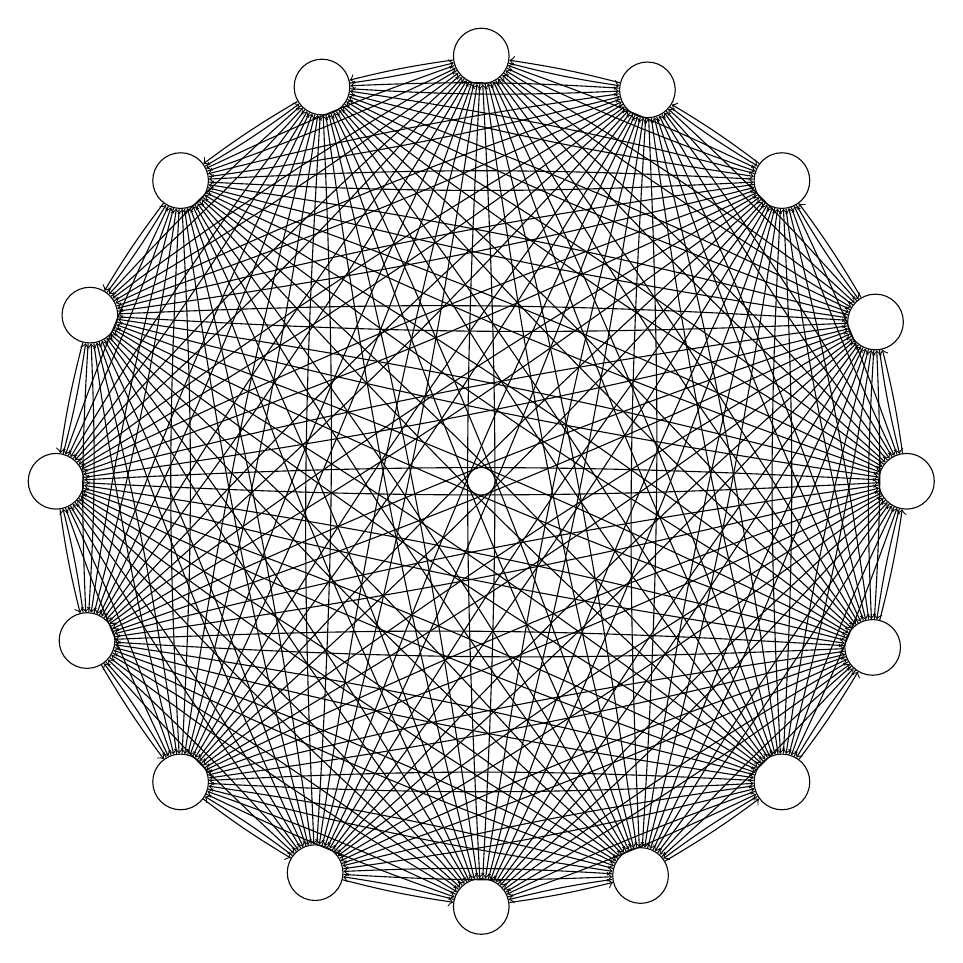
\begin{tikzpicture}[transform shape]
  %the multiplication with floats is not possible. Thus I split the loop in two.
  \foreach \number in {1,...,8}{
      % Computer angle:
        \mycount=\number
        \advance\mycount by -1
  \multiply\mycount by 45
        \advance\mycount by 0
      \node[draw,circle,inner sep=0.25cm] (N-\number) at (\the\mycount:5.4cm) {};
    }
  \foreach \number in {9,...,16}{
      % Computer angle:
        \mycount=\number
        \advance\mycount by -1
  \multiply\mycount by 45
        \advance\mycount by 22.5
      \node[draw,circle,inner sep=0.25cm] (N-\number) at (\the\mycount:5.4cm) {};
    }
  \foreach \number in {1,...,15}{
        \mycount=\number
        \advance\mycount by 1
  \foreach \numbera in {\the\mycount,...,16}{
    \path (N-\number) edge[->,bend right=3] (N-\numbera)  edge[<-,bend
      left=3] (N-\numbera);
  }
}
\end{tikzpicture}

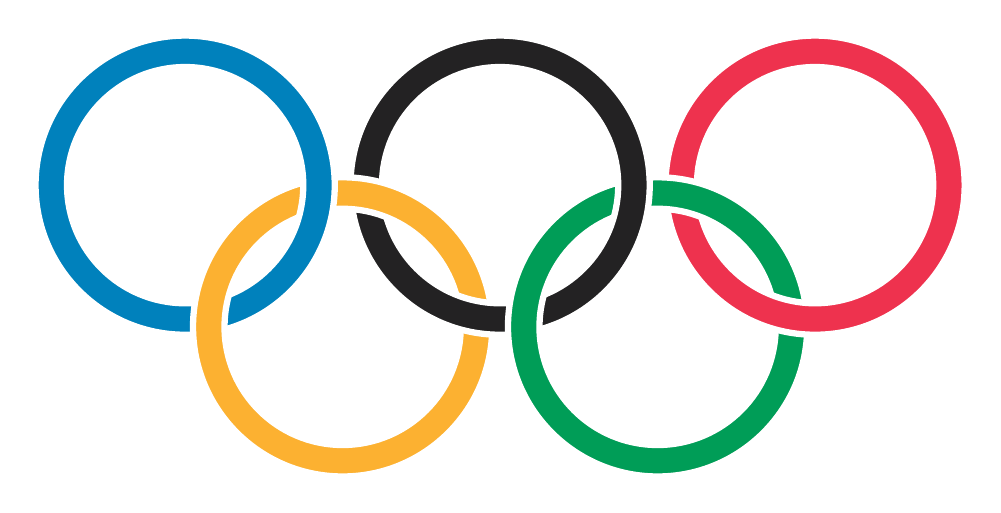
\begin{tikzpicture}
 \definecolor{r1}{RGB}{0,129,188}
 \definecolor{r2}{RGB}{252,177,49}
 \definecolor{r3}{RGB}{35,34,35}
 \definecolor{r4}{RGB}{0,157,87}
 \definecolor{r5}{RGB}{238,50,78}
 \begin{scope}
   \clip (-6,2) rectangle (6,-.9);
   \foreach \col/\xp/\yp in {
     r5/4/0, r4/2/-1.8, r3/0/0,
     r2/-2/-1.8, r1/-4/0
   } {
     \path[draw=white,line width=.08cm,
     fill=\col,even odd rule]
     (\xp, \yp) circle (1.9cm)
     (\xp, \yp) circle (1.5cm);
   }
 \end{scope}
 \begin{scope}
   \clip (-6,-.9) rectangle (6,-3.8);
   \foreach \col/\xp/\yp in {
     r1/-4/0, r2/-2/-1.8, r3/0/0,
     r4/2/-1.8, r5/4/0
   } {
     \path[draw=white,line width=.08cm,
     fill=\col,even odd rule]
     (\xp, \yp) circle (1.9cm)
     (\xp, \yp) circle (1.5cm);
   }
 \end{scope}
\end{tikzpicture}


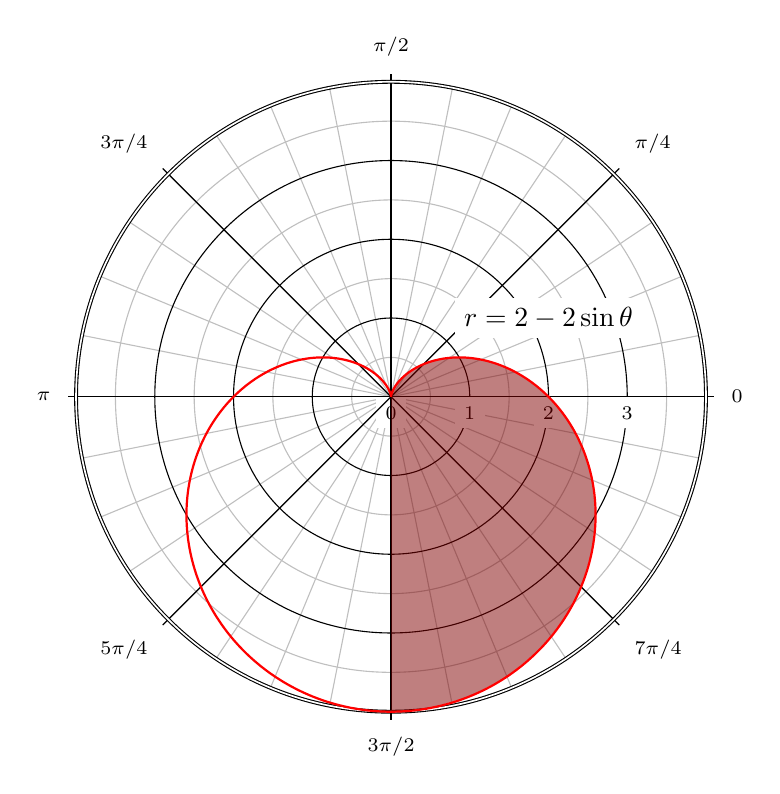
\begin{tikzpicture}[>=latex]

% Draw the lines at multiples of pi/12
\foreach \ang in {0,...,31} {
  \draw [lightgray] (0,0) -- (\ang * 180 / 16:4);
}

% Concentric circles and radius labels
\foreach \s in {0, 1, 2, 3} {
  \draw [lightgray] (0,0) circle (\s + 0.5);
  \draw (0,0) circle (\s);
  \node [fill=white] at (\s, 0) [below] {\scriptsize $\s$};
}

% Add the labels at multiples of pi/4
\foreach \ang/\lab/\dir in {
  0/0/right,
  1/{\pi/4}/{above right},
  2/{\pi/2}/above,
  3/{3\pi/4}/{above left},
  4/{\pi}/left,
  5/{5\pi/4}/{below left},
  7/{7\pi/4}/{below right},
  6/{3\pi/2}/below} {
  \draw (0,0) -- (\ang * 180 / 4:4.1);
  \node [fill=white] at (\ang * 180 / 4:4.2) [\dir] {\scriptsize $\lab$};
}

% The double-lined circle around the whole diagram
\draw [style=double] (0,0) circle (4);

\fill [fill=red!50!black, opacity=0.5] plot [domain=-pi/2:pi/2]
  (xy polar cs:angle=\x r, radius= {2-2*sin(\x r)});
\draw [thick, color=red, domain=0:2*pi, samples=200, smooth]
  plot (xy polar cs:angle=\x r, radius={2-2*sin(\x r)});
\node [fill=white] at (2,1) {$r=2-2\sin\theta$};

\end{tikzpicture} 


% definition de partial ellipse
\tikzset{partial ellipse/.style args =
  {#1:#2:#3}{insert path={+ (#1:#3) arc (#1:#2:#3)}}}
\begin{tikzpicture}[>=latex]
  %  ellipses
  \draw [fill=white!90!red]    (3,-1.8) ellipse    (4cm and 1 cm);
  \draw [fill=yellow!90!green] (3,-1.8) ellipse (3cm and 0.75 cm);
  \draw [fill=white!90!green]  (3,-1.8) ellipse  (2cm and 0.5 cm);

  % -- Soleil
  \shade [ball color=gray!10!yellow] (3,-1.8) circle (1);
  \node (soleil) at (3,-1.8) {\bf Soleil};
  % partial ellipse pour tracé devant le Soleil
  \draw (3,-1.8) [partial ellipse=220:320:2cm and 0.5cm]
        (3,-1.8) [partial ellipse=220:320:3cm and 0.75cm];

  % Venus
  \shade [ball color=gray!10!orange] (1.6,-1.8) circle (.2);
  \node (venus) at (1.5,-1.45) {Venus}; 

  % ombre de Venus
  \draw[color=white!70!black,fill=white!70!black]
    (1.6,-2.3) ellipse (2mm and 0.5mm);

  % Mercure
  \shade [ball color=gray!10!orange] (5,-1.225) circle (.25);
  \node (mercure) at (5,-0.8) {Mercure}; 

  % Earth
  \shade [ball color=white!50!blue] (5.75,-2.5) circle (.33);
  \node (terre) at (6.6,-2.6) {\bf Terre};

  % Lune
  \shade [ball color=yellow] (5.25,-2.8) circle (.1);
  \node (lune) at (5.25,-3) {Lune};
     
  % Mars
  \draw (3,-1.8) [partial ellipse=45:120:9cm and 2.5cm];
  \shade [ball color=black!50!red] (5,0.66) circle (.15);
  \node (mars) at (5,1) {\bf Mars};   
  % trajet
  \draw [line width=2pt,blue,->,>=latex] (terre) to[out=0,in=0] (mars);   
\end{tikzpicture}
\end{center}


\end{document}
